\label{chpt:evaluation}
This chapter evaluates the quality and performance of the ray tracing algorithm
presented in Chapter~\ref{chpt:implementation} using the San Miguel scene
introduced in Chapter~\ref{chpt:design}.  Four different numbers of voxels are
tested against different numbers of nodes on a distributed system with eight
nodes, each with an 8-core Intel Xeon processor.

\section{Test Case}
The San Miguel scene is traced using a global ambient light and a directional
luminaire to produce an output image of size 2400$\times$1600.  The scene is
small enough to run on a single node of our system which allows us create a baseline
to compare our algorithm against by tracing the entire scene on a single node.
Distributions of 1 voxel (baseline), 9 voxels, 27 voxels and 64 voxels are
tested on 1 node, 2 nodes, 4 nodes, and 8 nodes.  The number of triangles per
voxel are shown in Figure~\ref{fig:voxel-distributions}.
Section~\ref{sec:quality} evaluates the quality of the test case and
Section~\ref{sec:performance} evaluates the performance.

\begin{figure}[!htb]
\noindent\makebox[\textwidth]{%
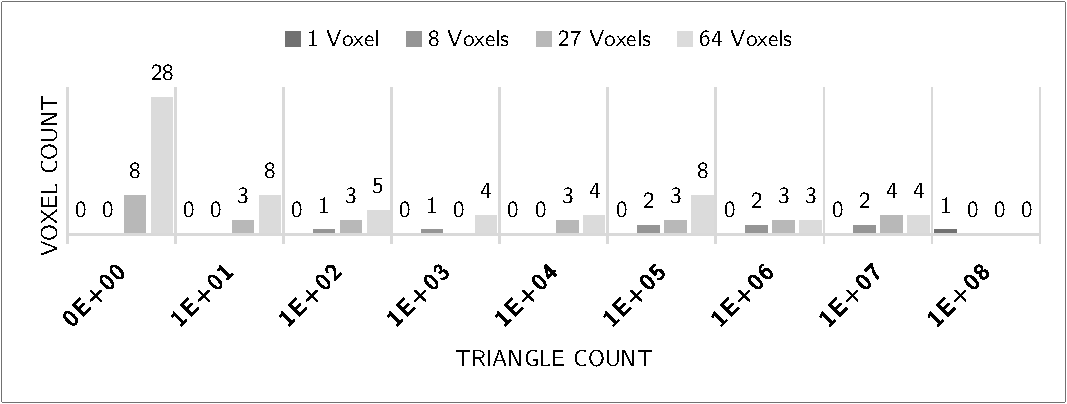
\includegraphics[width=6in]{drawings/test_case/All.pdf}
}
\caption{San Miguel - Scene Distribution for Test Cases}
\label{fig:voxel-distributions}
\end{figure}

\section{Image Quality}
\label{sec:quality}
\subsection{Baseline}
Figure~\ref{fig:san-miguel-1}a shows the baseline ray traced San Miguel scene
using an unmodified version of Embree.  Figure~\ref{fig:san-miguel-1}b and
Figure~\ref{fig:san-miguel-1}c show the resulting traced images for the ambient
light and the directional luminaire, respectively, from tracing a single voxel.
Figure~\ref{fig:san-miguel-1}d shows the composited image produced by combining
Figure~\ref{fig:san-miguel-1}a and Figure~\ref{fig:san-miguel-1}b.  As no rays
intersect objects outside the single traced voxel, the image produces is
identical to the baseline.

\begin{figure}[!htb]
\setlength\tabcolsep{0pt}
\noindent\makebox[\textwidth]{%
\begin{tabular}{ c c c }
\fcolorbox{wsu-gray}{white}{%
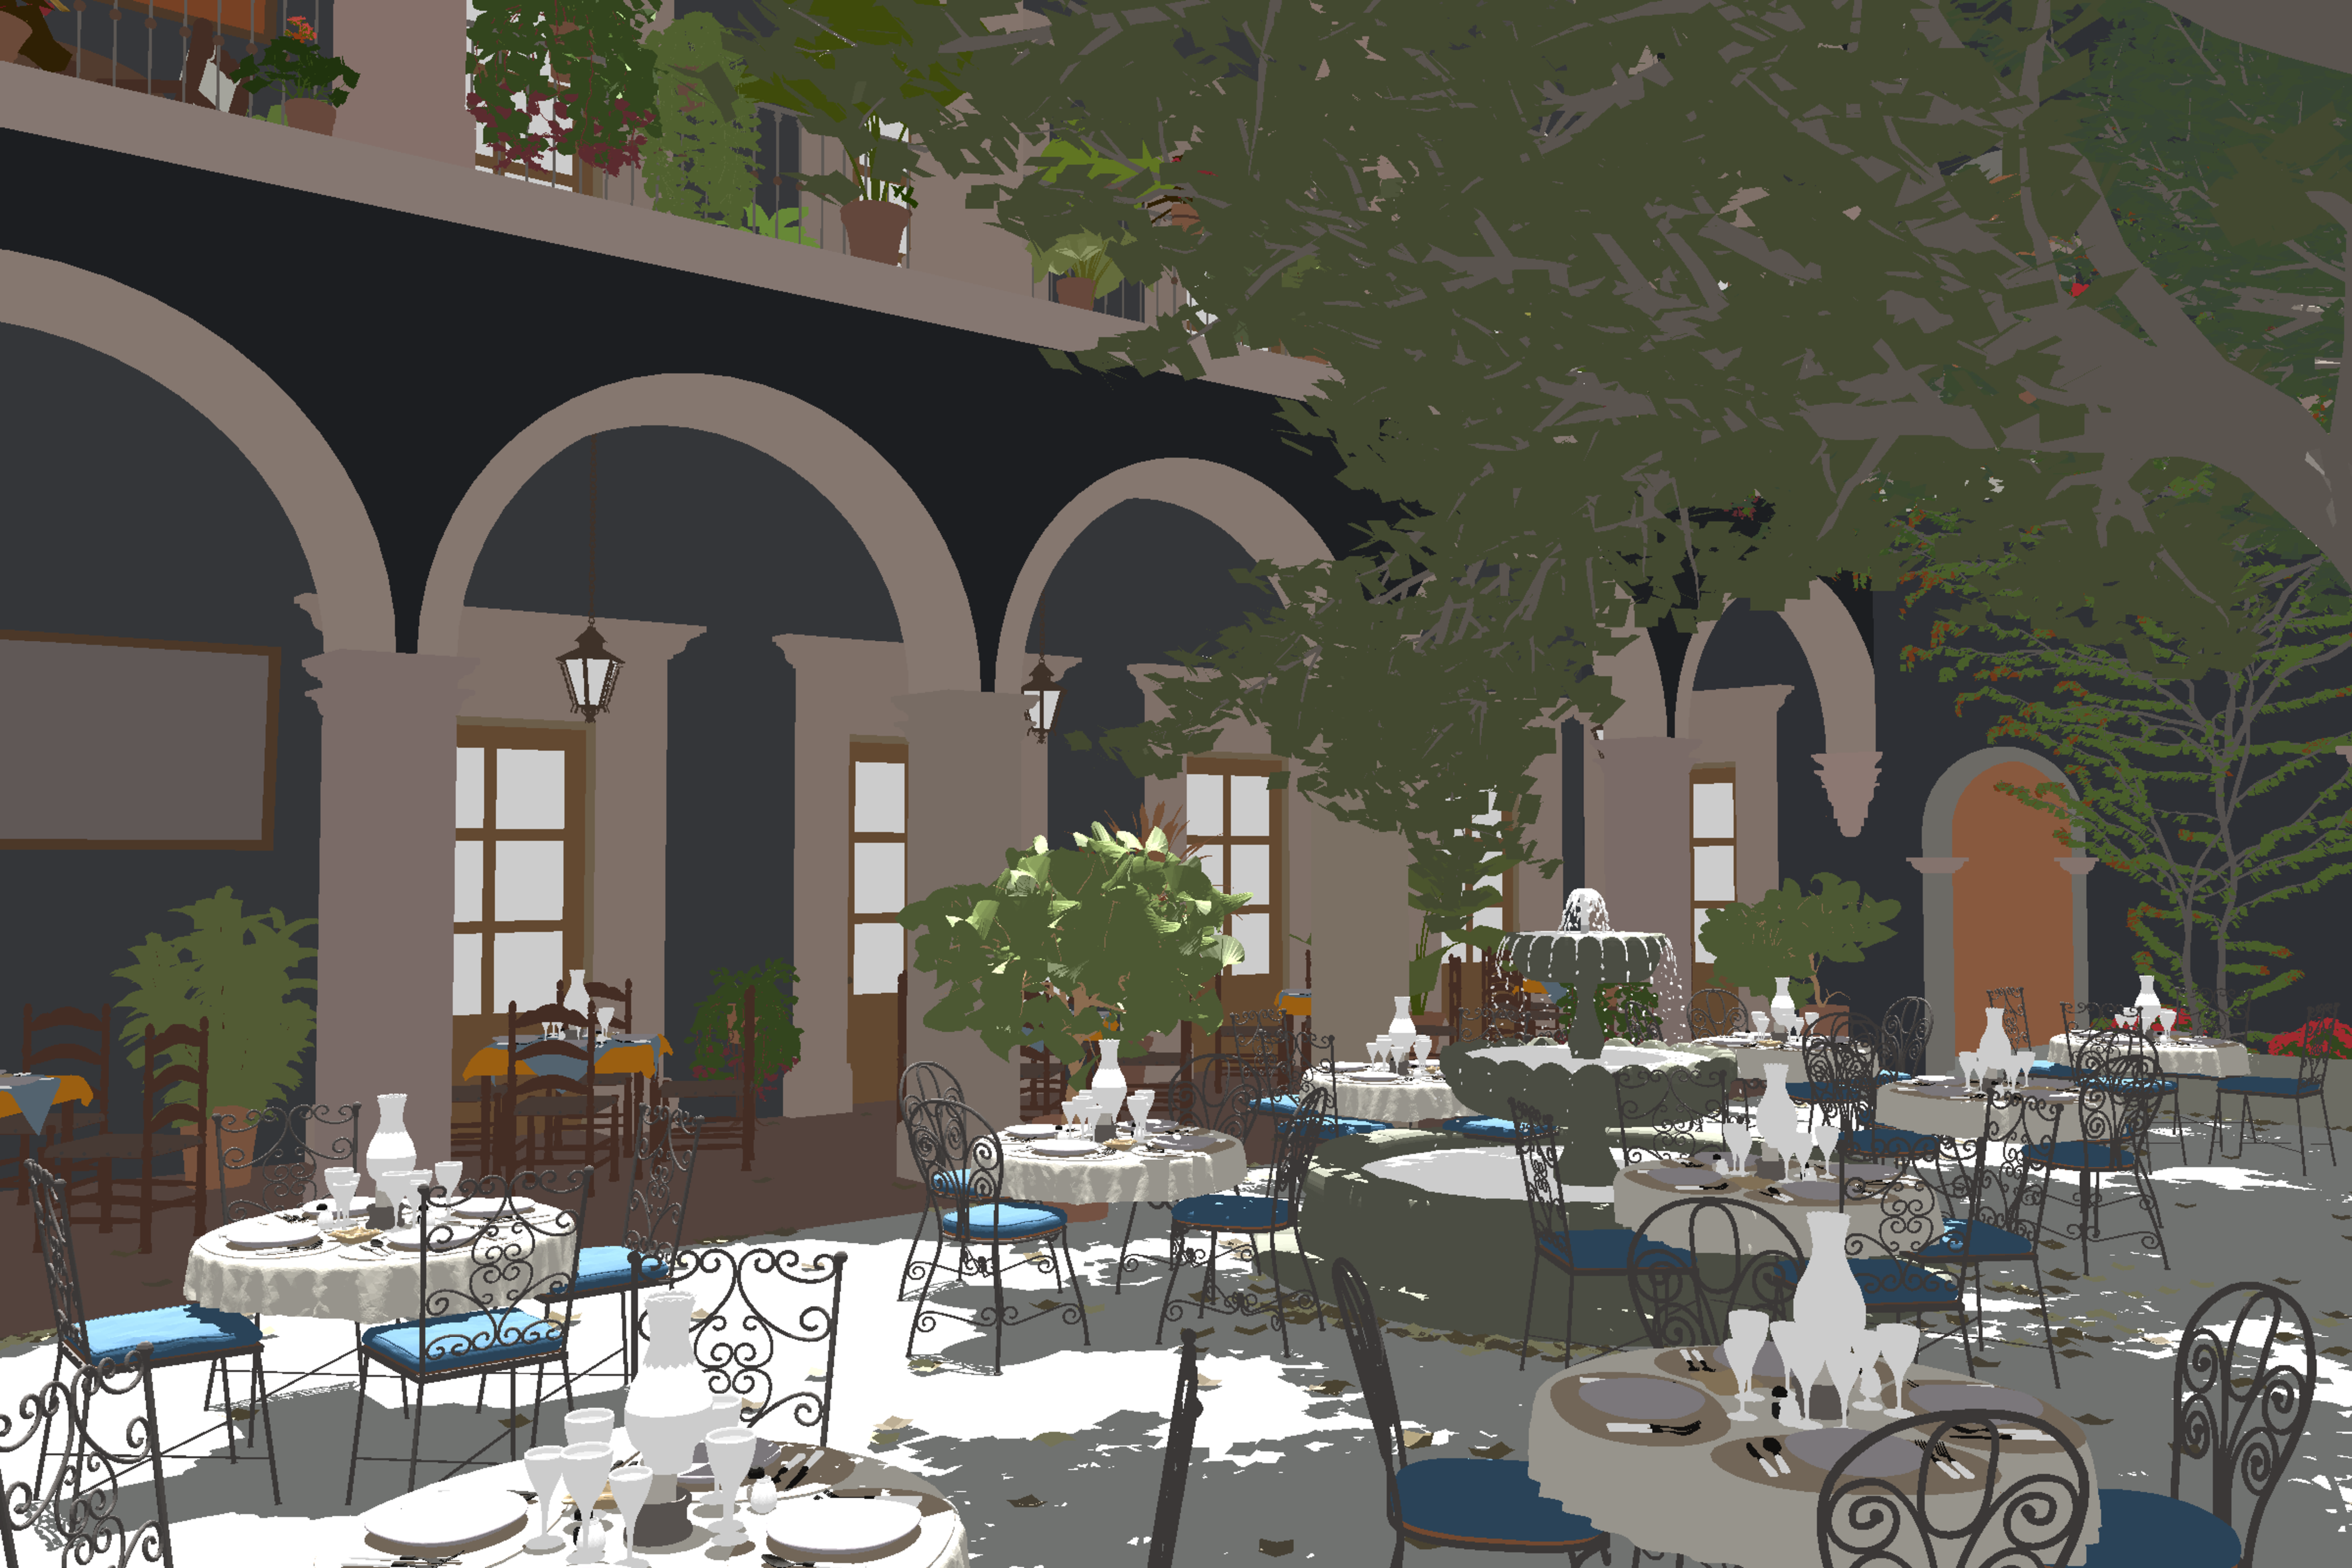
\includegraphics[width=3in]{drawings/test_case/results/san_miguel_1_traced.pdf}%
}
& \hspace{0.1in} &
\fcolorbox{wsu-gray}{white}{%
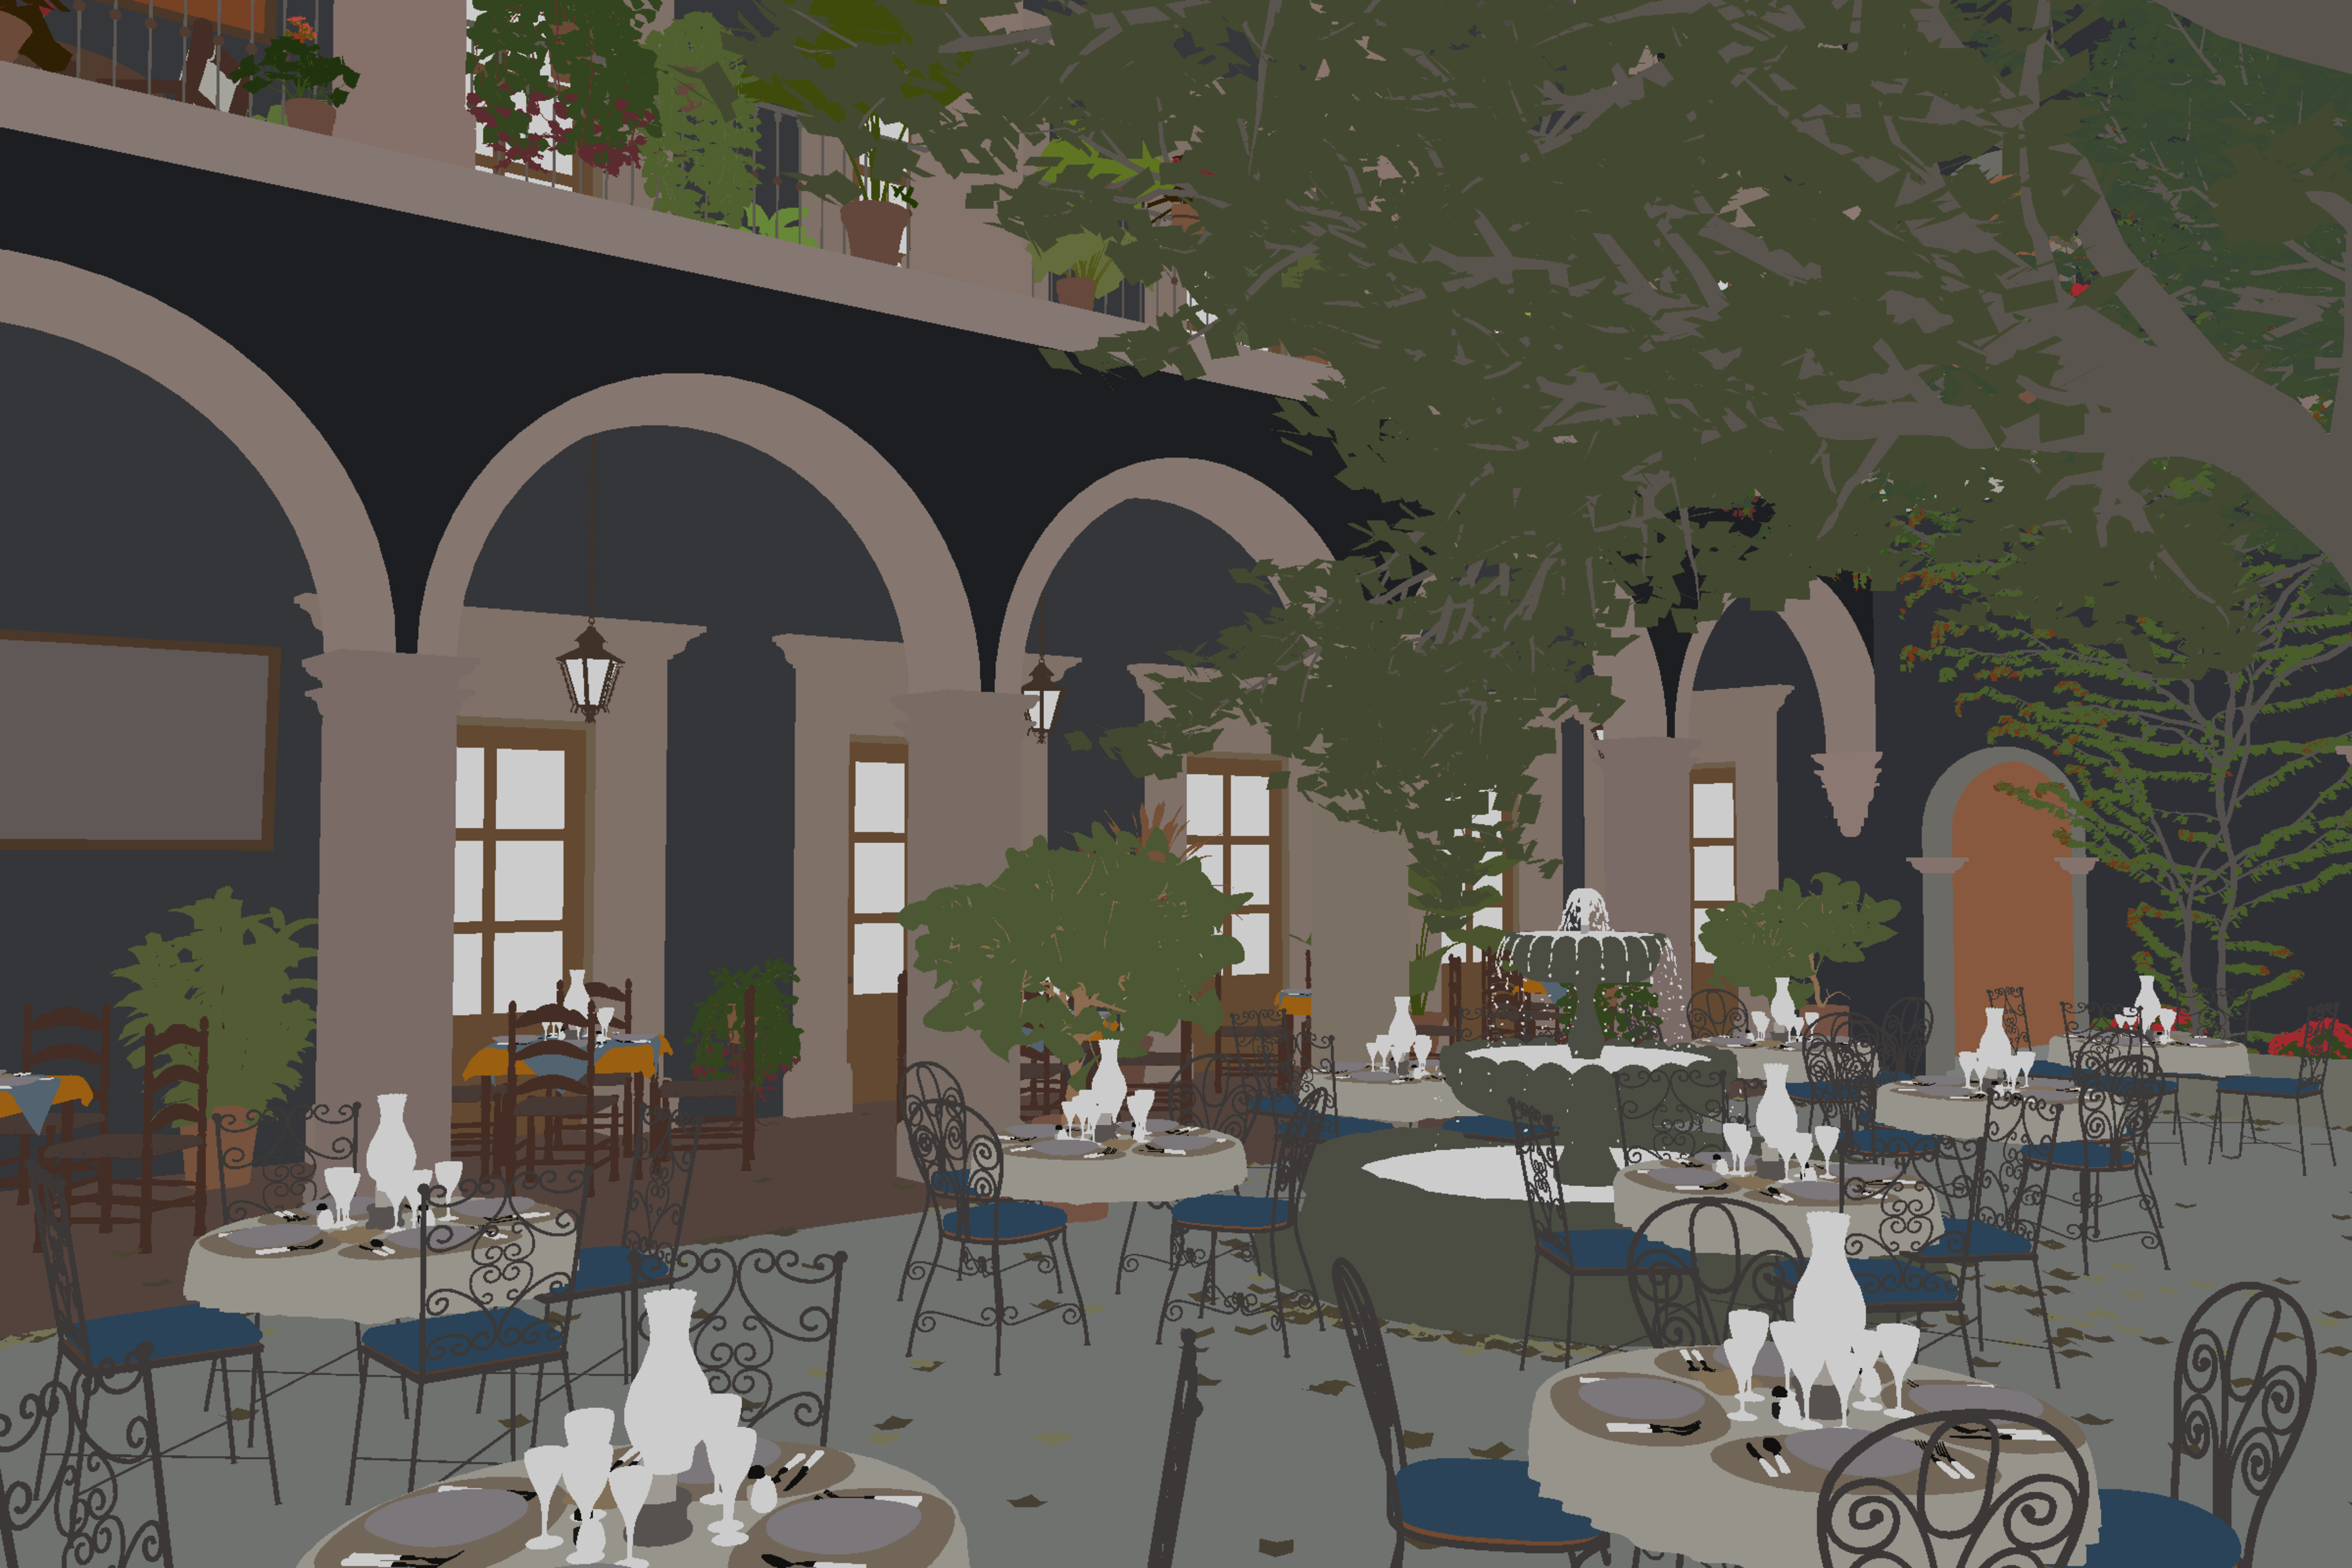
\includegraphics[width=3in]{drawings/test_case/results/san_miguel_1_ambient.pdf}%
}
\\
(a) Ray Traced Image (Baseline) & \hspace{0.1in} & (b) Ambient Light Traced Image \\
\fcolorbox{wsu-gray}{white}{%
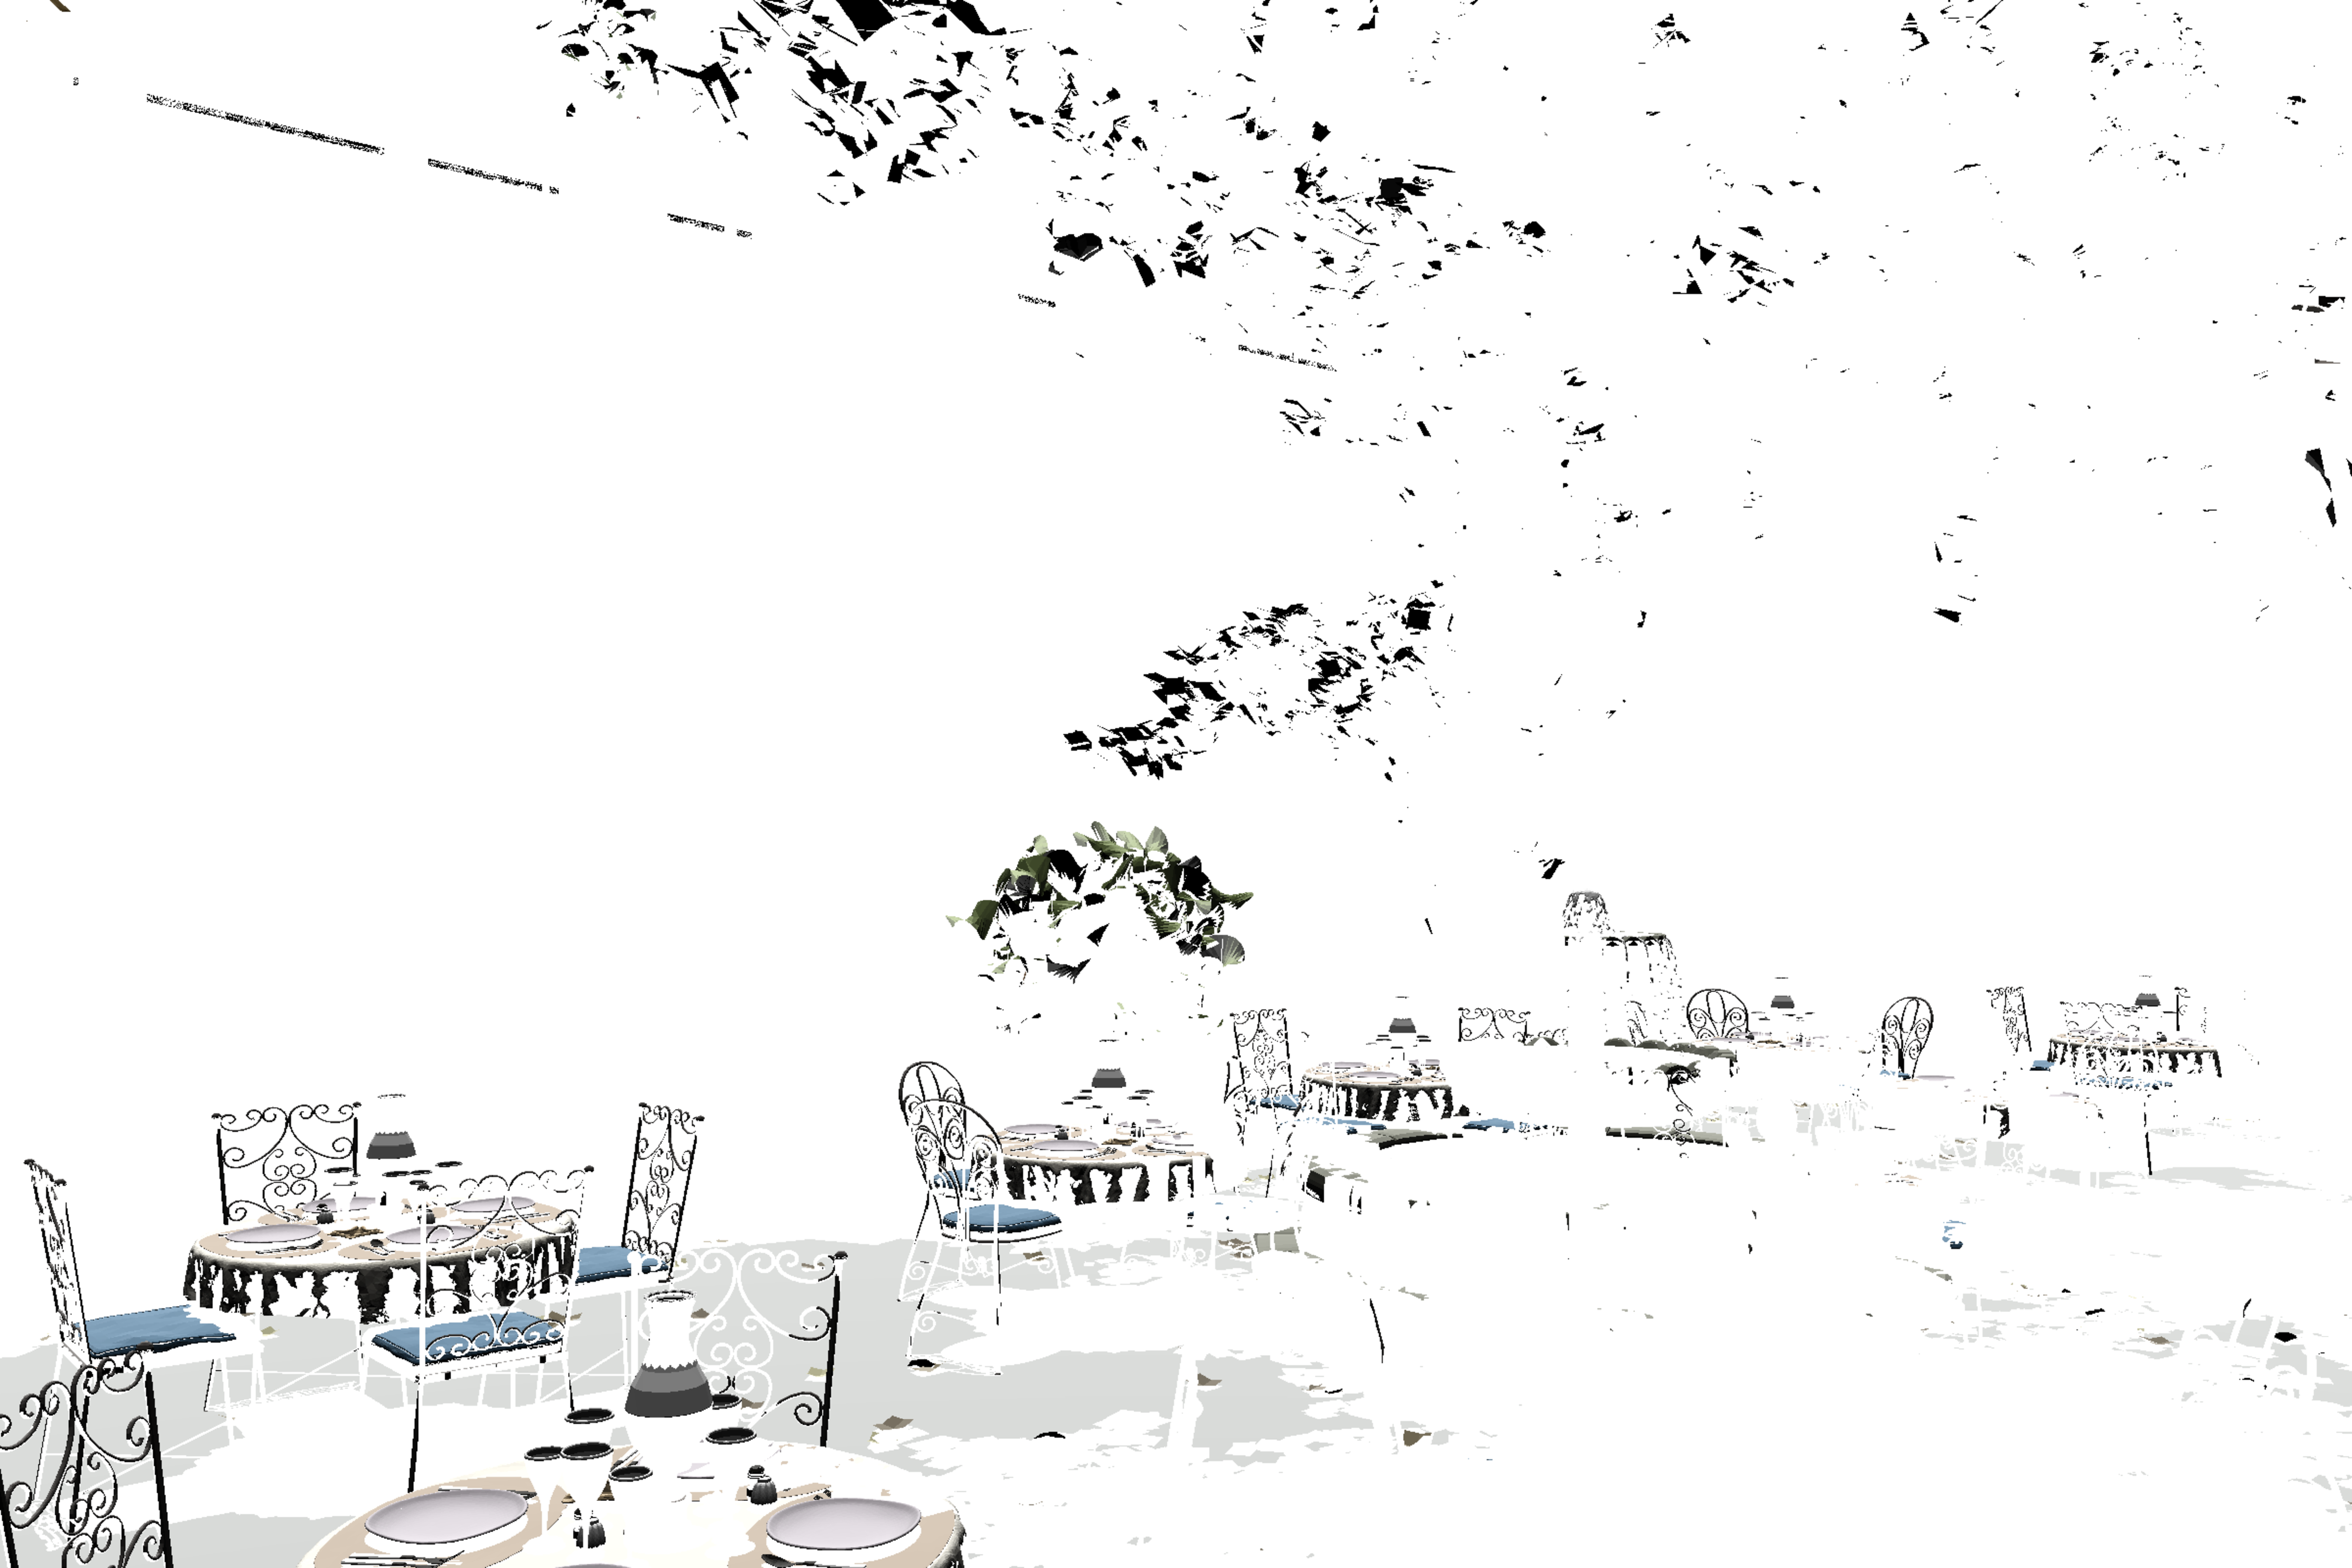
\includegraphics[width=3in]{drawings/test_case/results/san_miguel_1_light.pdf}%
}
& \hspace{0.1in} &
\fcolorbox{wsu-gray}{white}{%
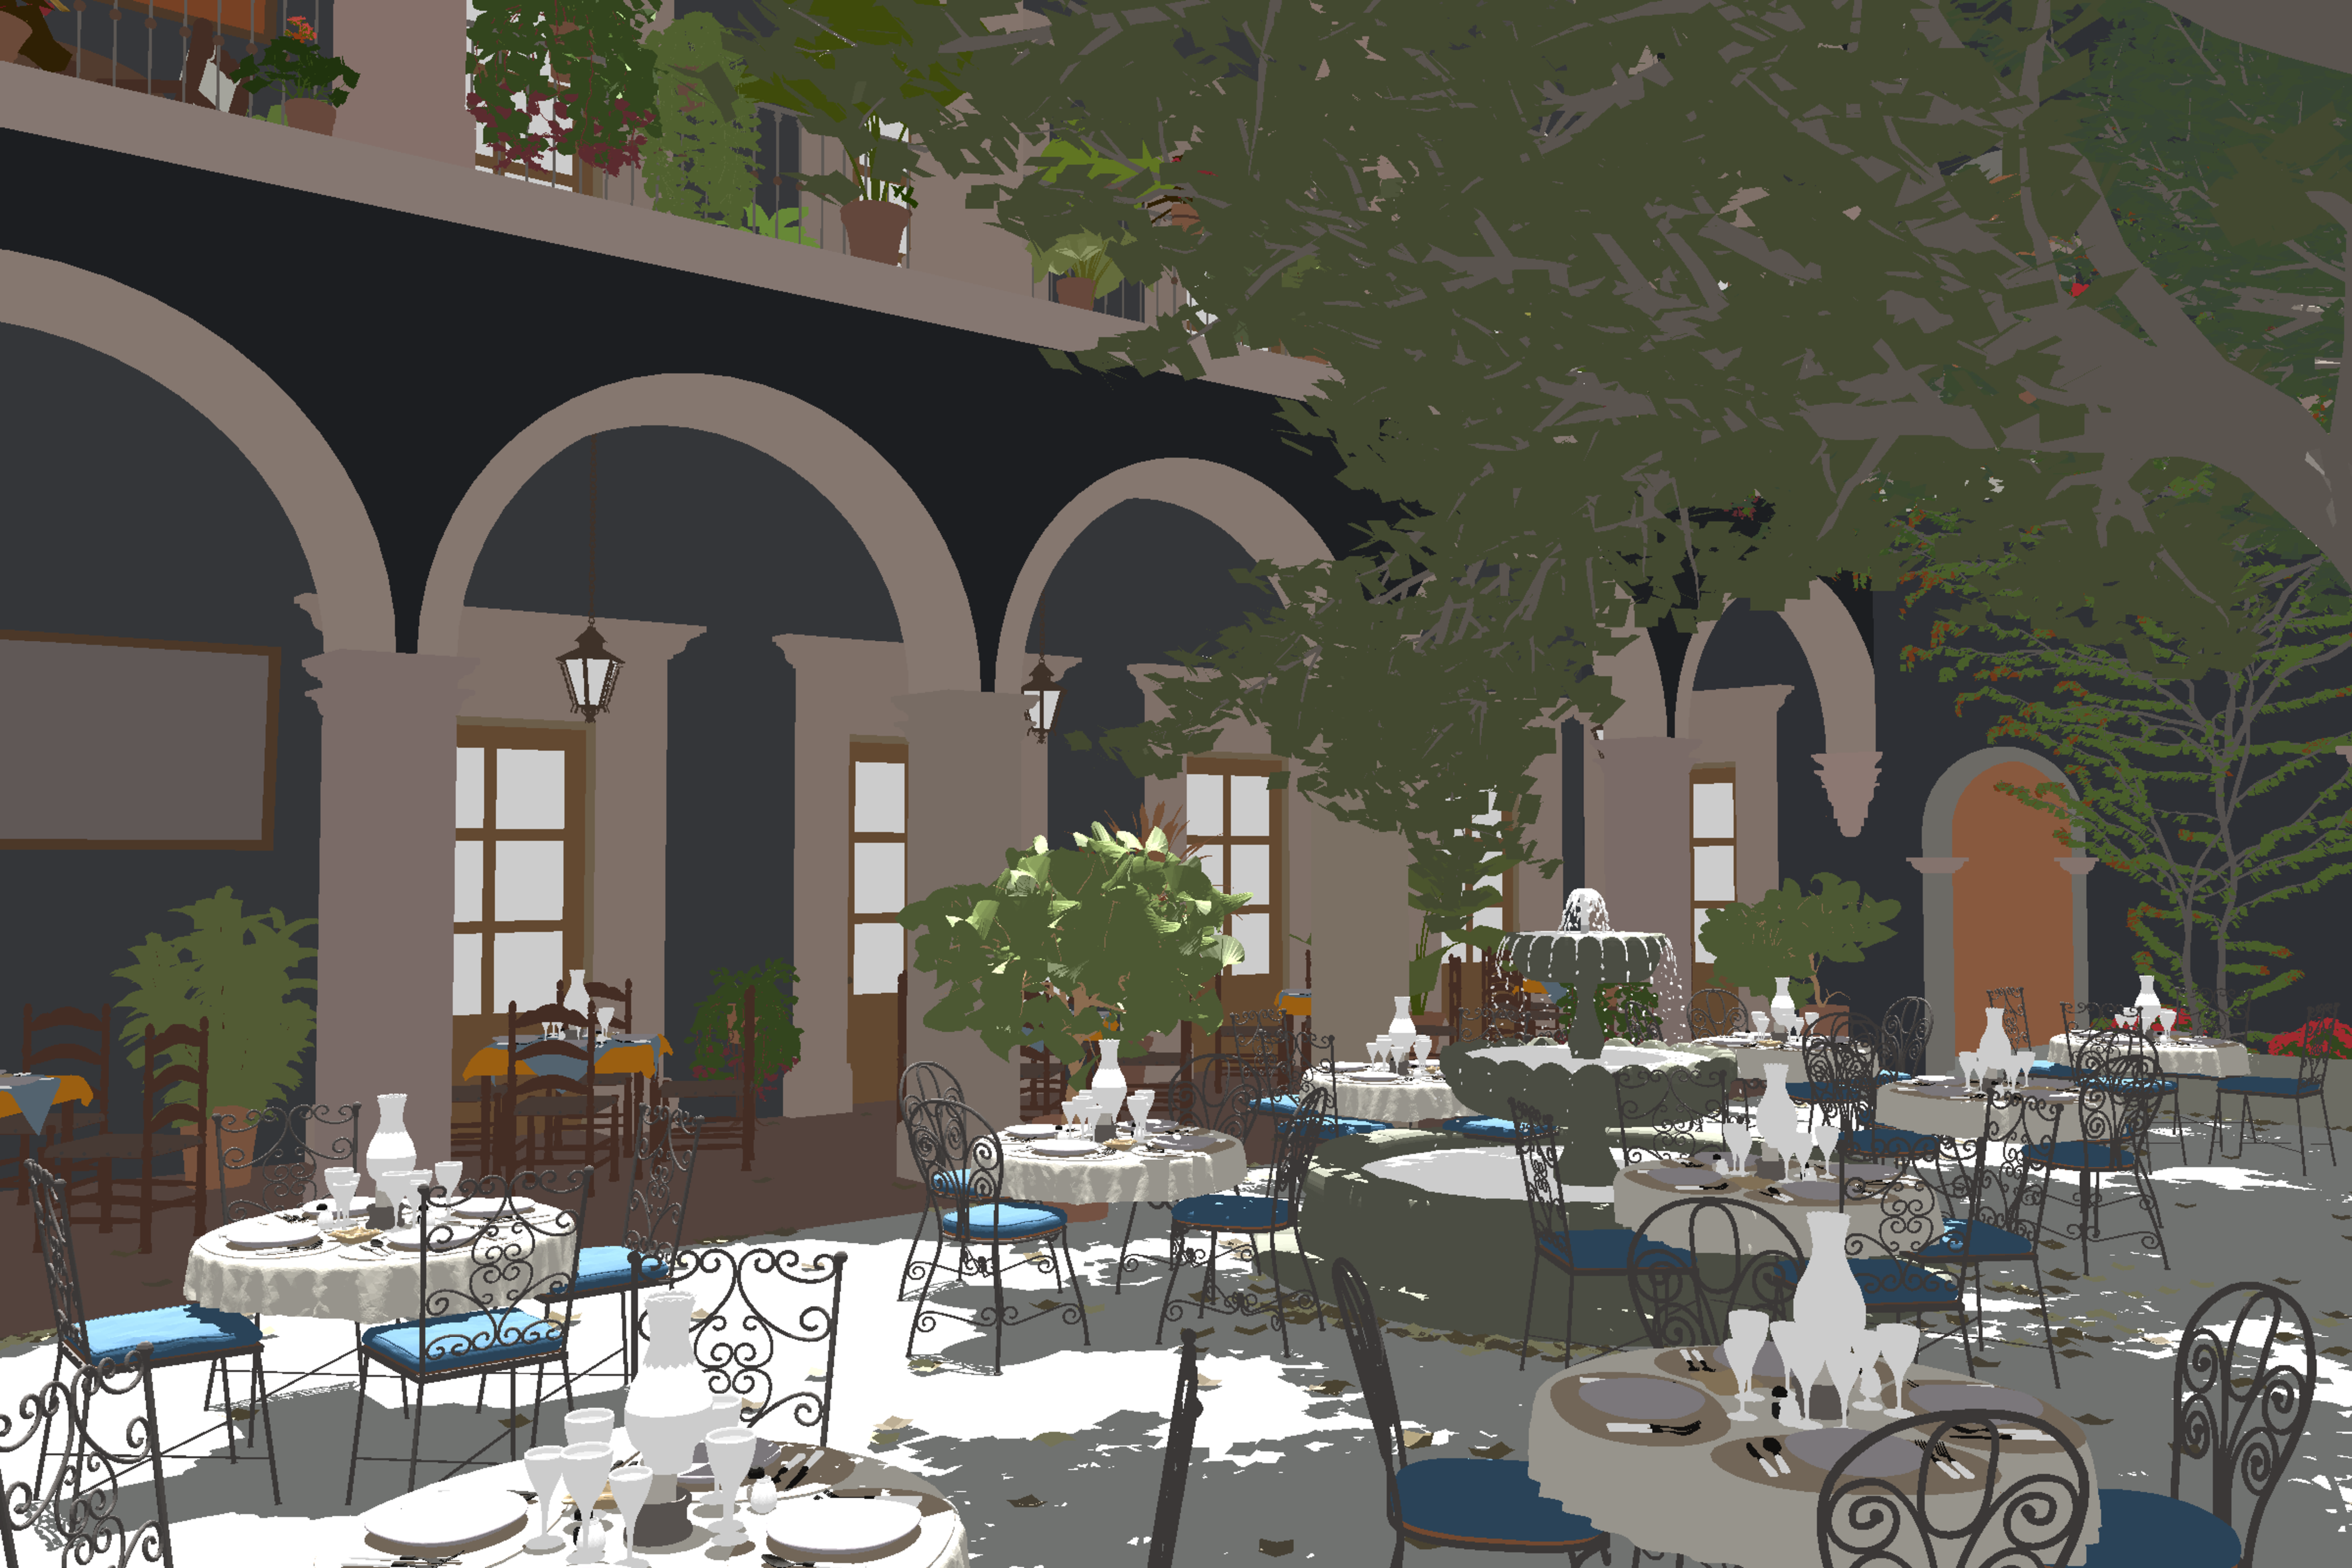
\includegraphics[width=3in]{drawings/test_case/results/san_miguel_1_traced.pdf}%
}
\\
(c) Point Luminaire Traced Image & \hspace{0.1in} & (d) Ray Traced Composite
Image
\end{tabular}}
\caption{San Miguel - Traced Image Output from 1-Voxel Test Case}
\label{fig:san-miguel-1}
\end{figure}

\subsection{8-Voxel Decomposition}
Figure~\ref{fig:san-miguel-8-image}a and Figure~\ref{fig:san-miguel-8-image}b
show the resulting traced images for the ambient light and the directional
luminaire, respectively, produced by \emph{trace viewing rays} for the San
Miguel scene split into 8 voxels. 

\begin{figure}[!htb]
\setlength\tabcolsep{0pt}
\noindent\makebox[\textwidth]{%
\begin{tabular}{ c c c c c c c }
\fcolorbox{wsu-gray}{white}{%
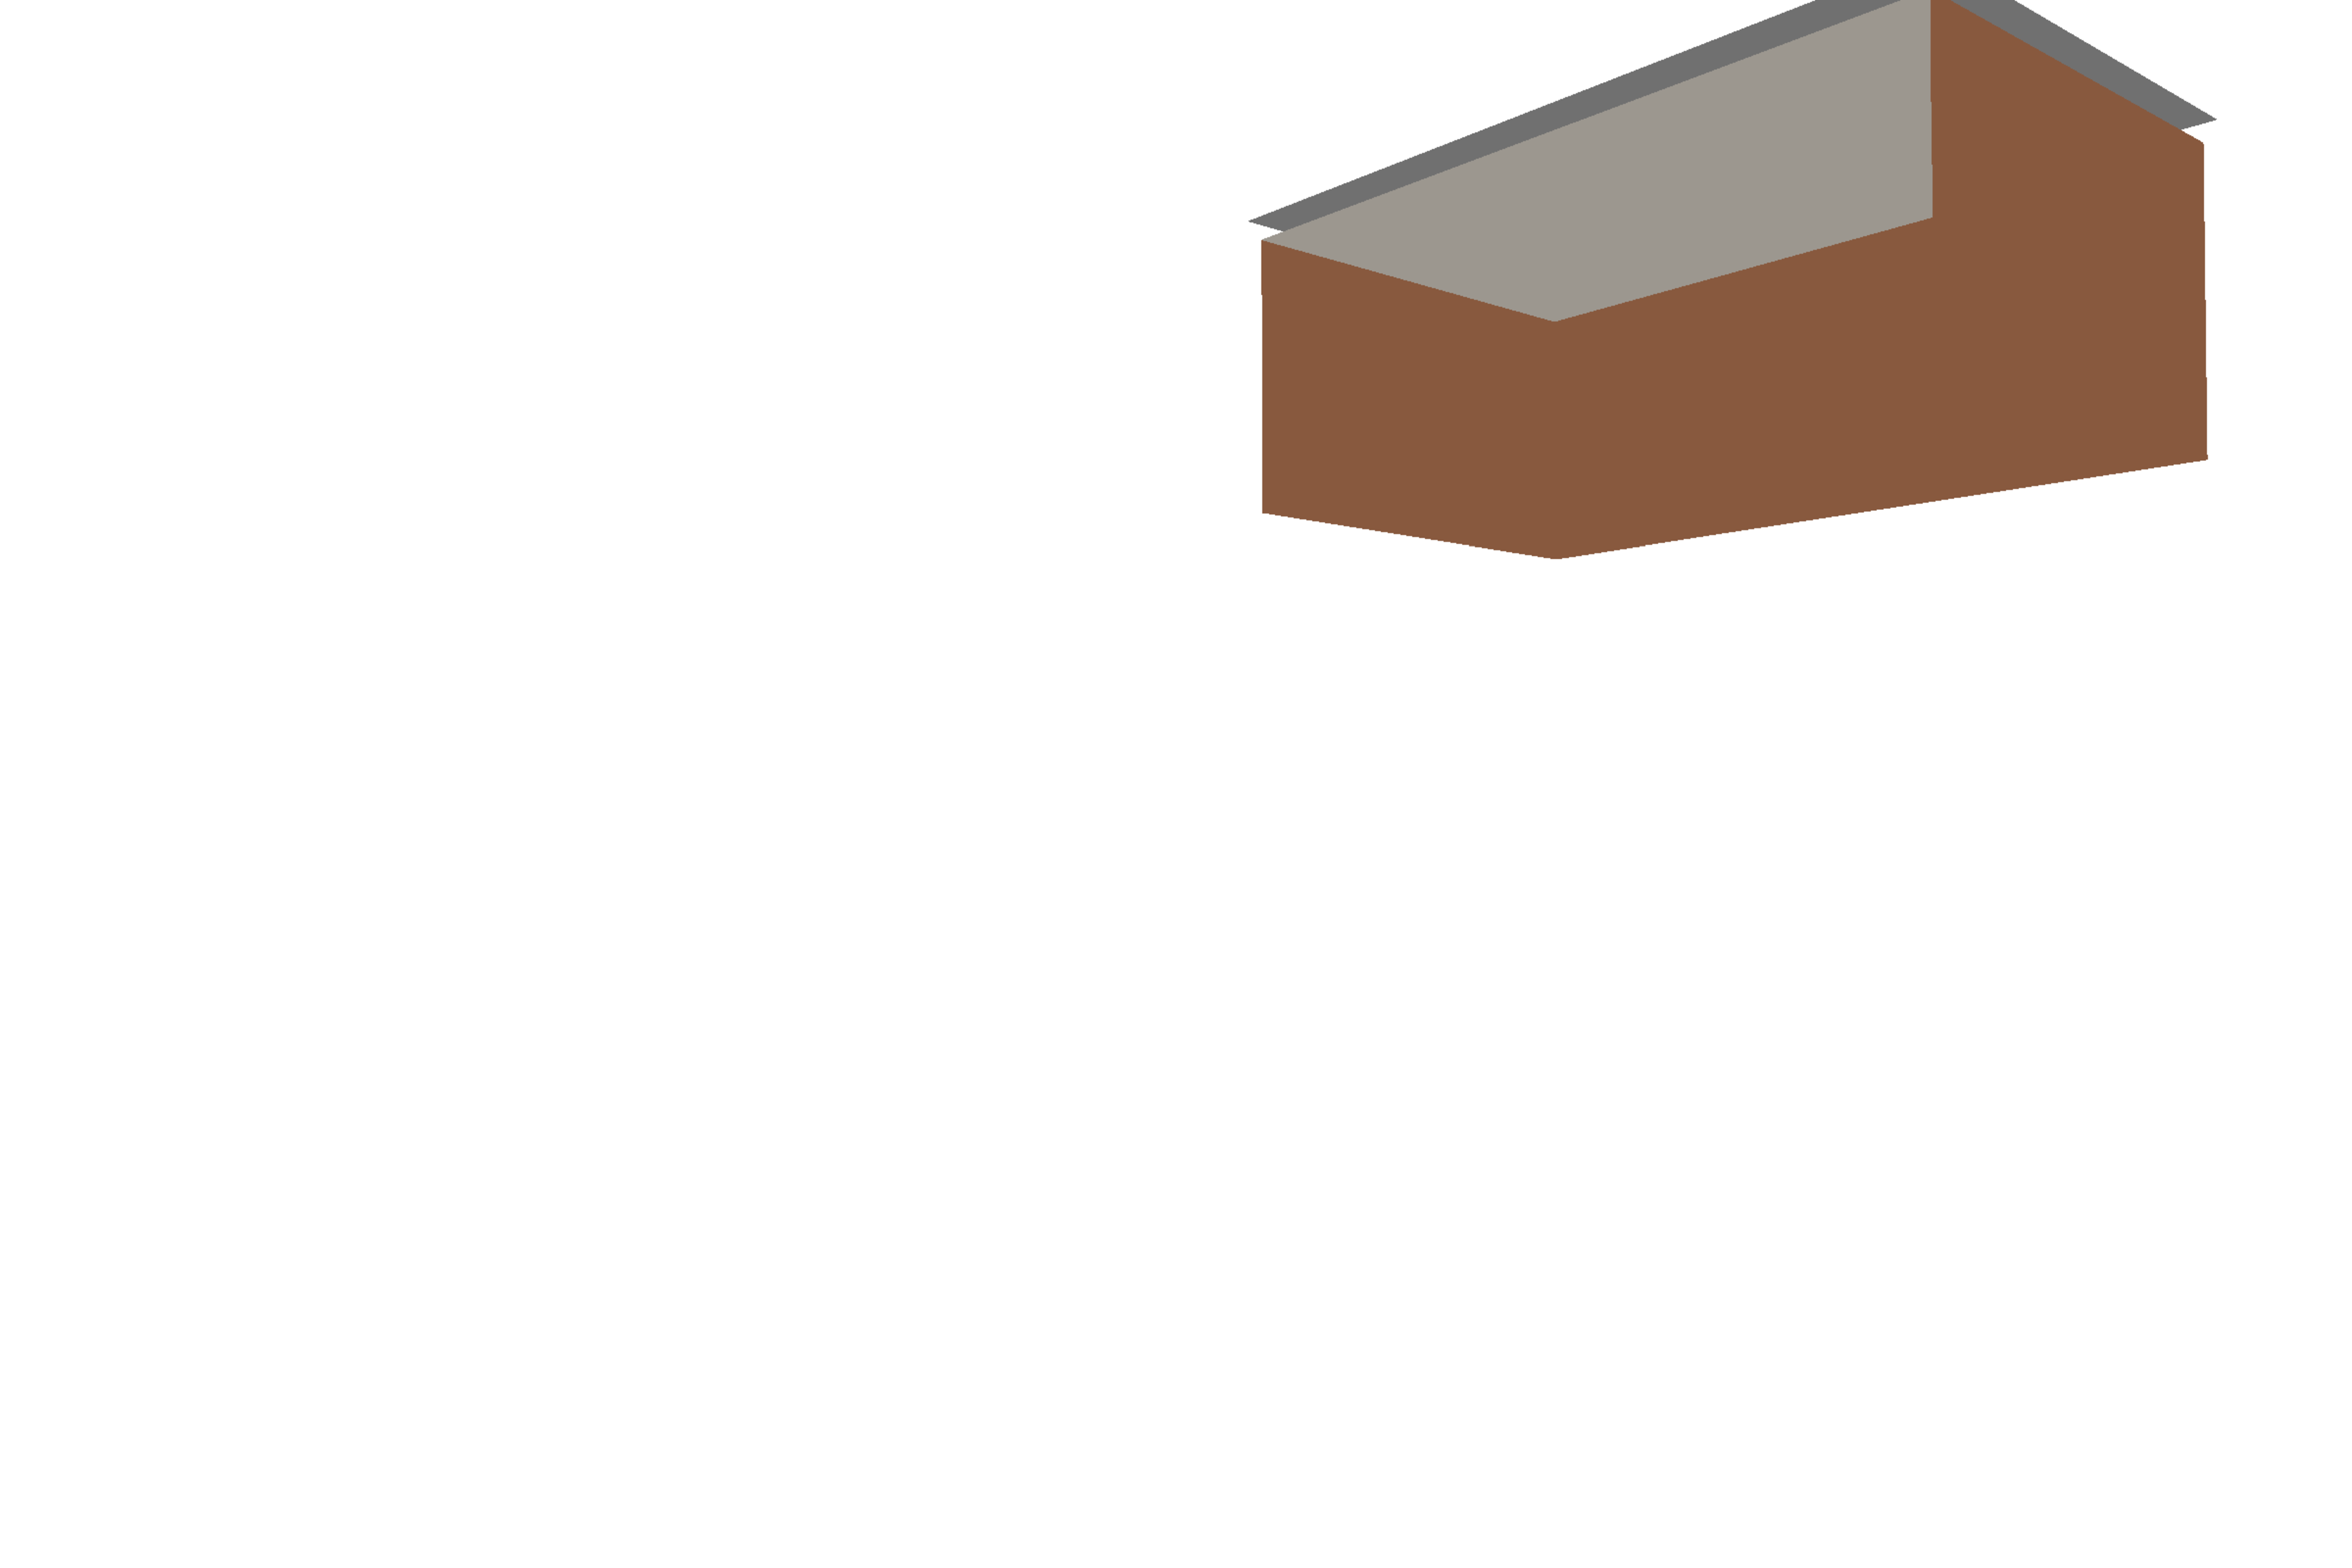
\includegraphics[width=1.5in]{drawings/test_case/results/san_miguel_8_3_ambient.pdf}%
}
& \hspace{0.1in} &
\fcolorbox{wsu-gray}{white}{%

\includegraphics[width=1.5in]{drawings/test_case/results/san_miguel_8_2_ambient.pdf}%
}
& \hspace{0.1in} &
\fcolorbox{wsu-gray}{white}{%

\includegraphics[width=1.5in]{drawings/test_case/results/san_miguel_8_7_ambient.pdf}%
}
& \hspace{0.1in} &
\fcolorbox{wsu-gray}{white}{%

\includegraphics[width=1.5in]{drawings/test_case/results/san_miguel_8_6_ambient.pdf}%
}
\\
(1, 1, 0) & \hspace{0.1in} & (0, 1, 0) & \hspace{0.1in} &
(1, 1, 1) & \hspace{0.1in} & (0, 1, 1)  \\
\fcolorbox{wsu-gray}{white}{%
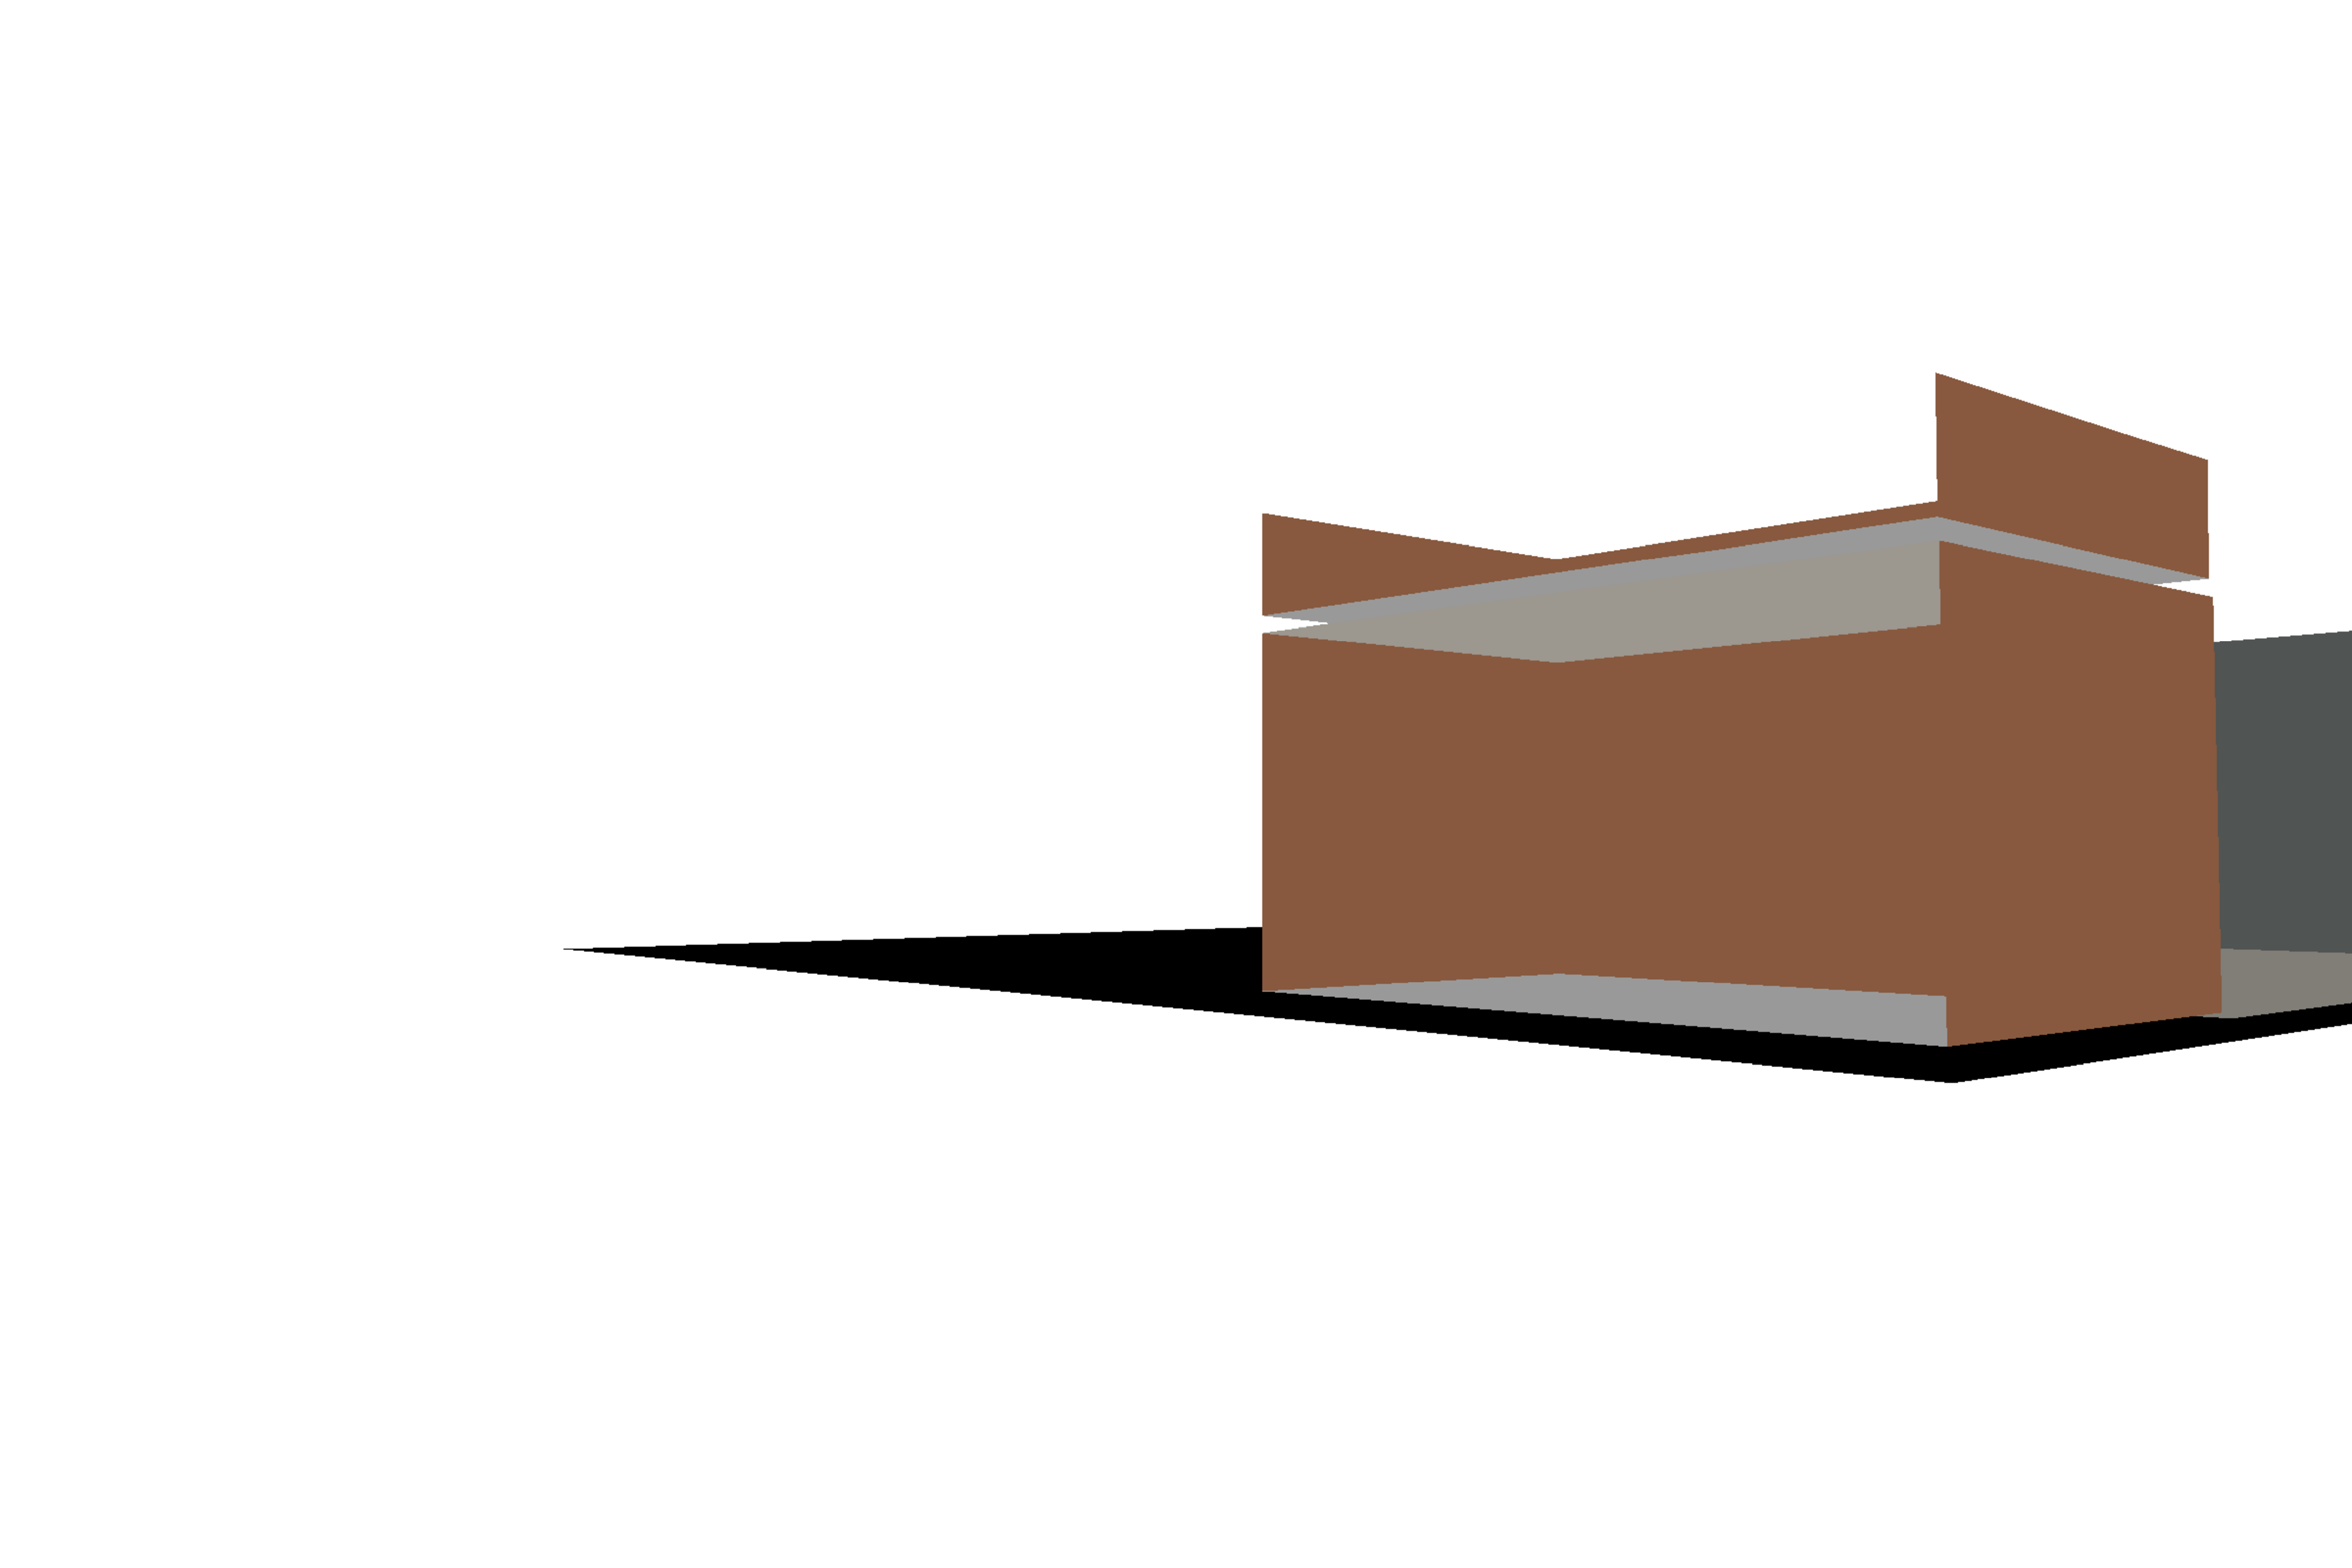
\includegraphics[width=1.5in]{drawings/test_case/results/san_miguel_8_1_ambient.pdf}%
}
& \hspace{0.1in} &
\fcolorbox{wsu-gray}{white}{%

\includegraphics[width=1.5in]{drawings/test_case/results/san_miguel_8_0_ambient.pdf}%
}
& \hspace{0.1in} &
\fcolorbox{wsu-gray}{white}{%
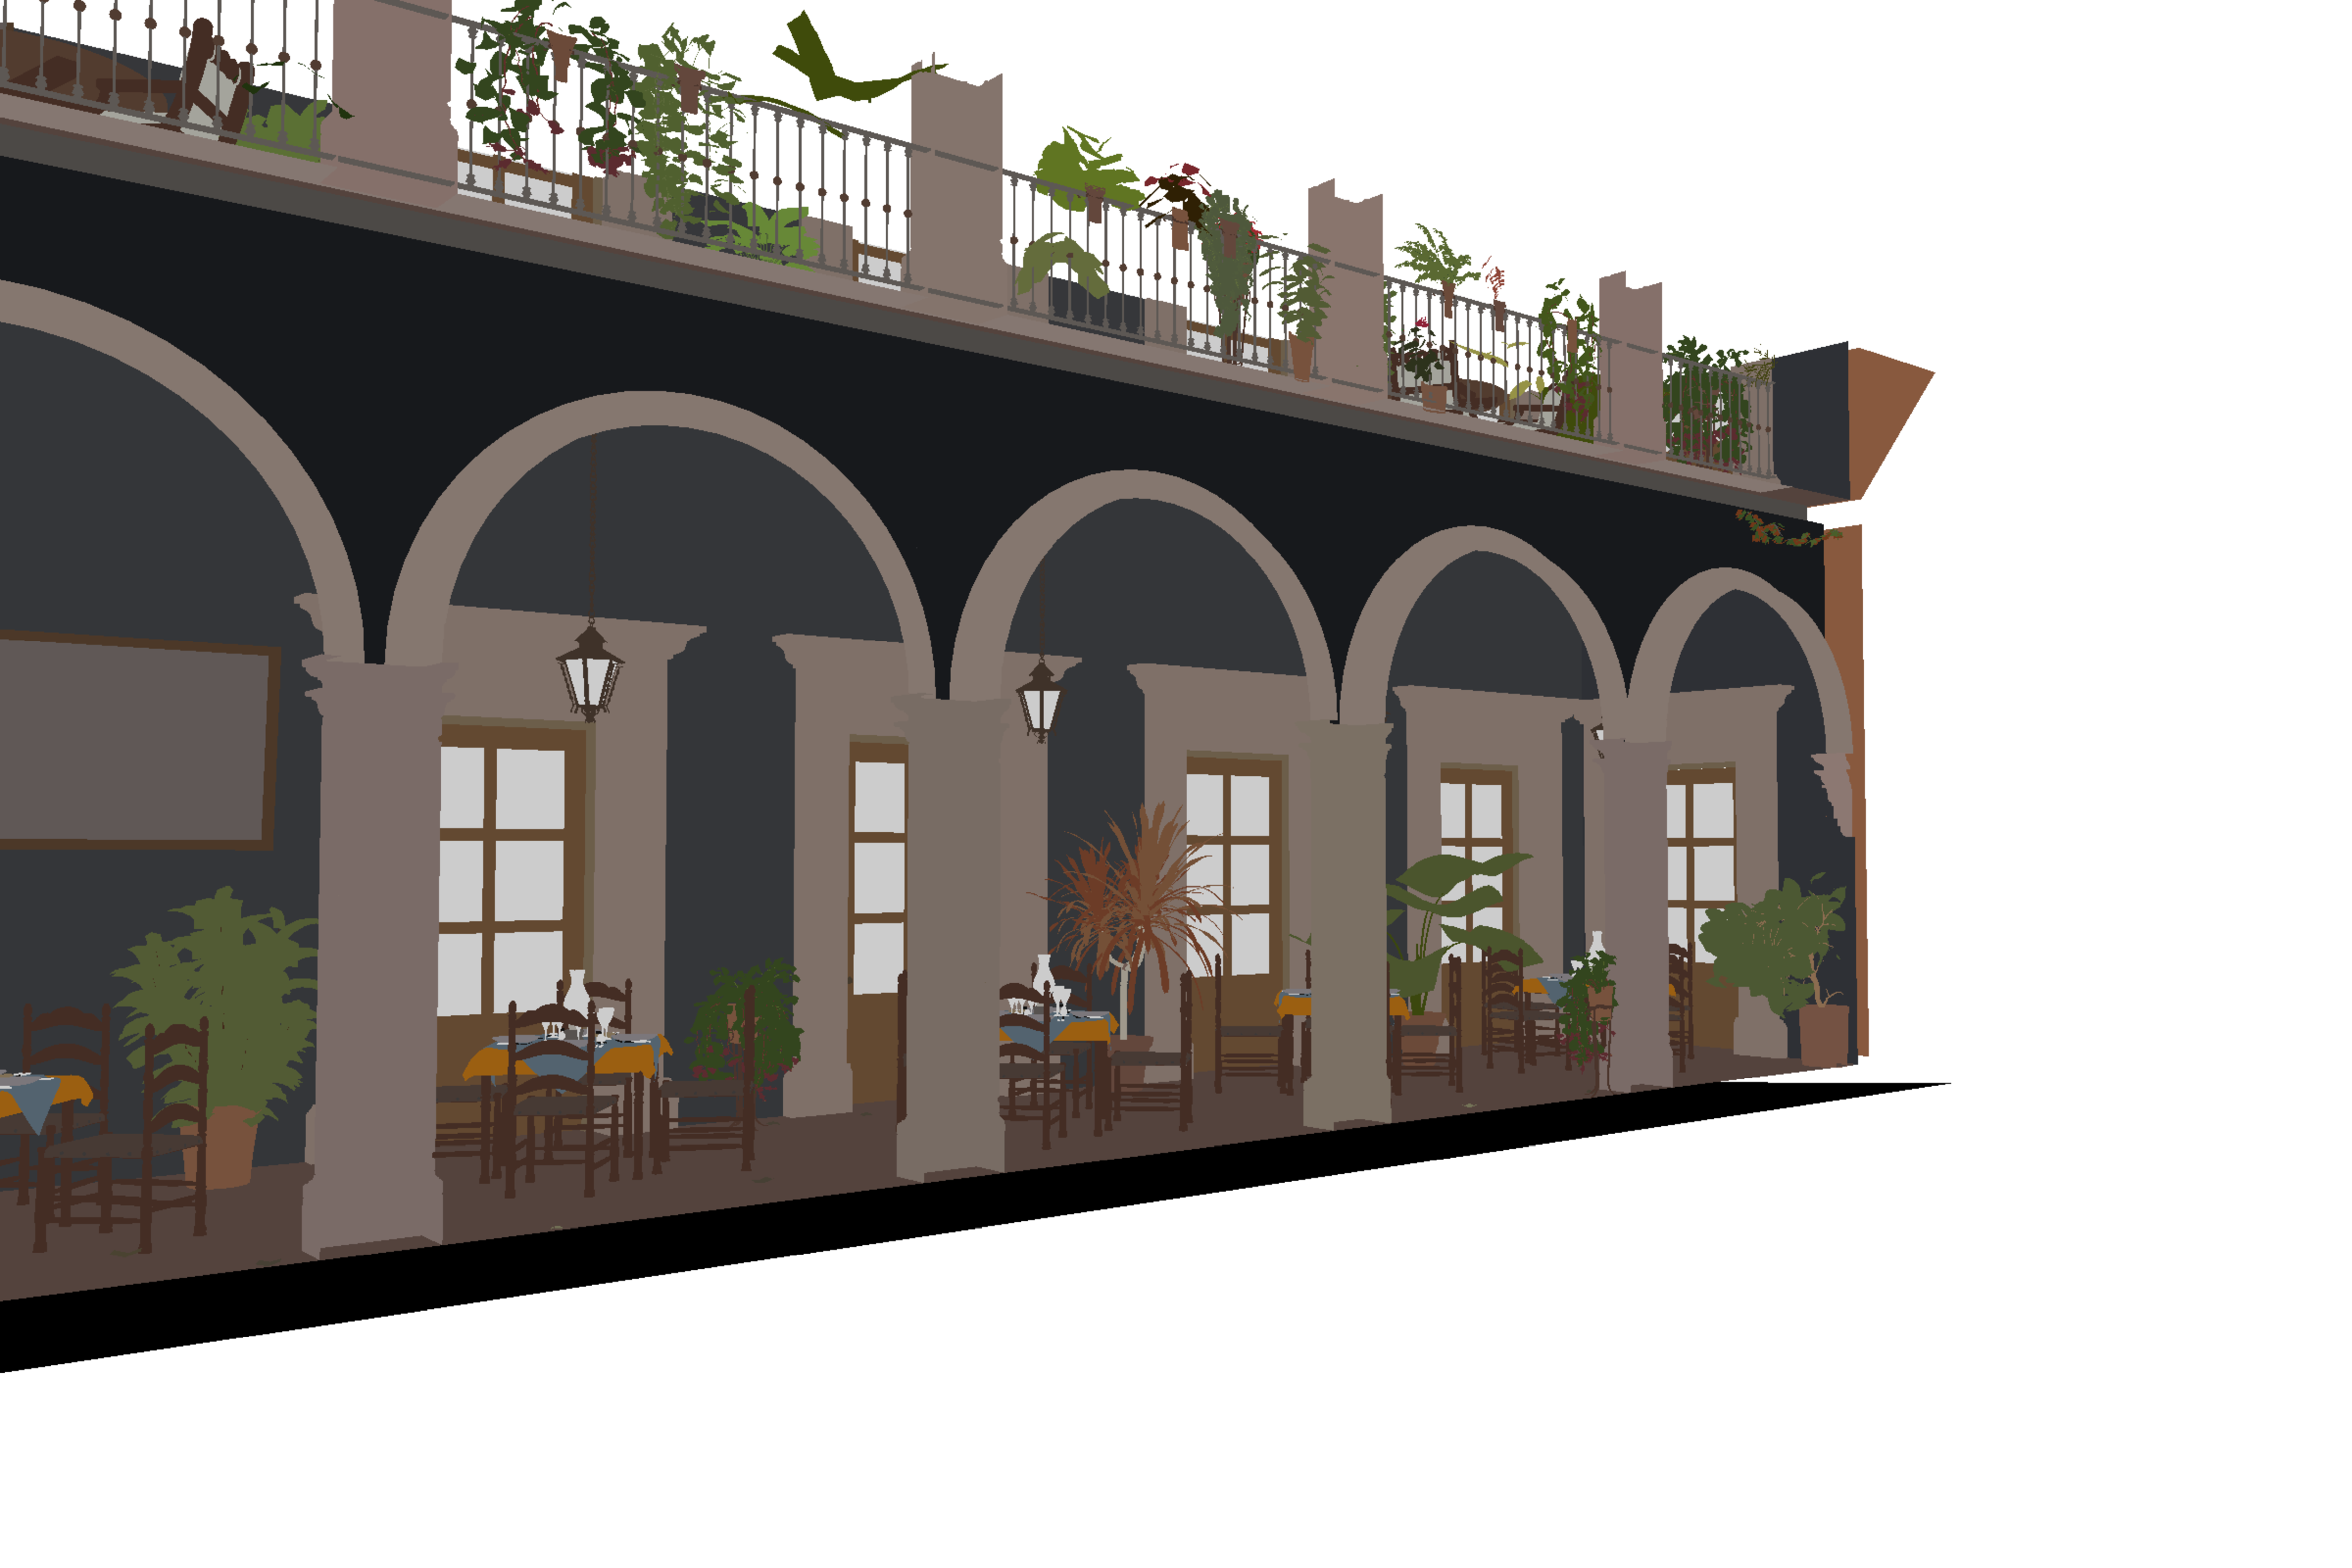
\includegraphics[width=1.5in]{drawings/test_case/results/san_miguel_8_5_ambient.pdf}%
}
& \hspace{0.1in} &
\fcolorbox{wsu-gray}{white}{%
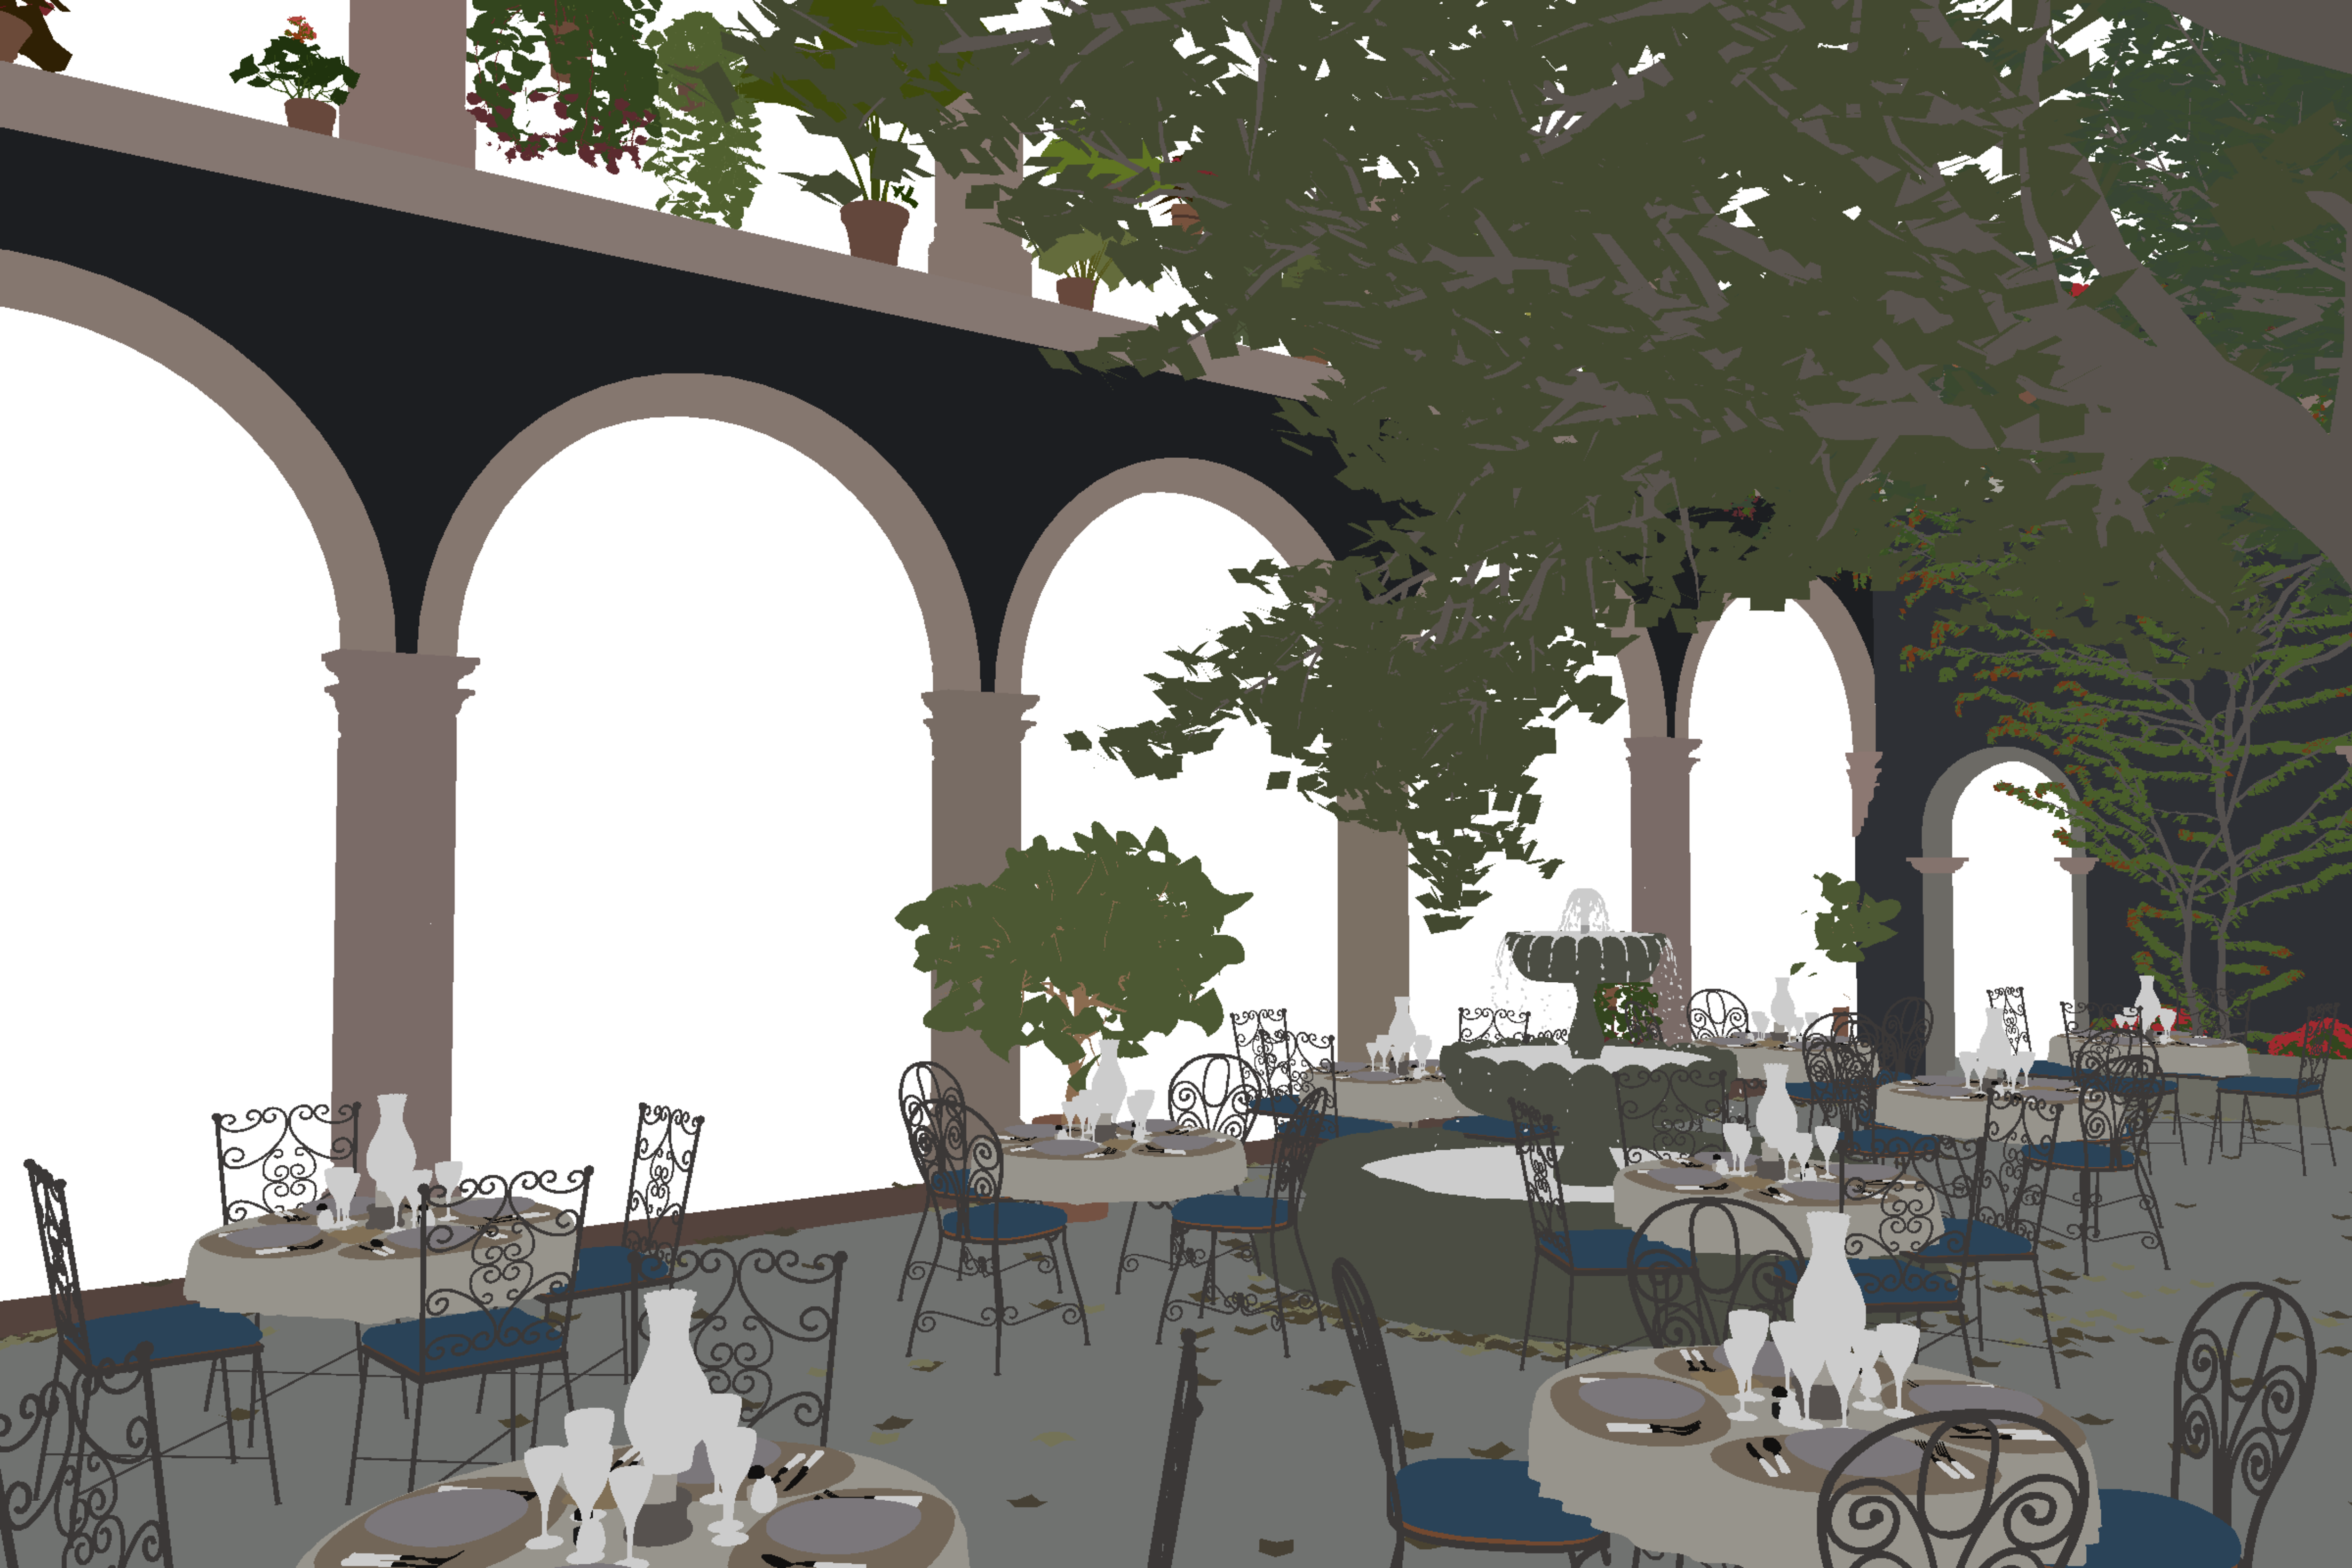
\includegraphics[width=1.5in]{drawings/test_case/results/san_miguel_8_4_ambient.pdf}%
}
\\
(1, 0, 0) & \hspace{0.1in} & (0, 0, 0) & \hspace{0.1in} &
(1, 0, 1) & \hspace{0.1in} & (0, 0, 1)  \\
\multicolumn{7}{c}{a) Ambient Light Traced Image Output} \\
\fcolorbox{wsu-gray}{white}{%

\includegraphics[width=1.5in]{drawings/test_case/results/san_miguel_8_3_light.pdf}%
}
& \hspace{0.1in} &
\fcolorbox{wsu-gray}{white}{%

\includegraphics[width=1.5in]{drawings/test_case/results/san_miguel_8_2_light.pdf}%
}
& \hspace{0.1in} &
\fcolorbox{wsu-gray}{white}{%

\includegraphics[width=1.5in]{drawings/test_case/results/san_miguel_8_7_light.pdf}%
}
& \hspace{0.1in} &
\fcolorbox{wsu-gray}{white}{%

\includegraphics[width=1.5in]{drawings/test_case/results/san_miguel_8_6_light.pdf}%
}
\\
(1, 1, 0) & \hspace{0.1in} & (0, 1, 0) & \hspace{0.1in} &
(1, 1, 1) & \hspace{0.1in} & (0, 1, 1)  \\
\fcolorbox{wsu-gray}{white}{%
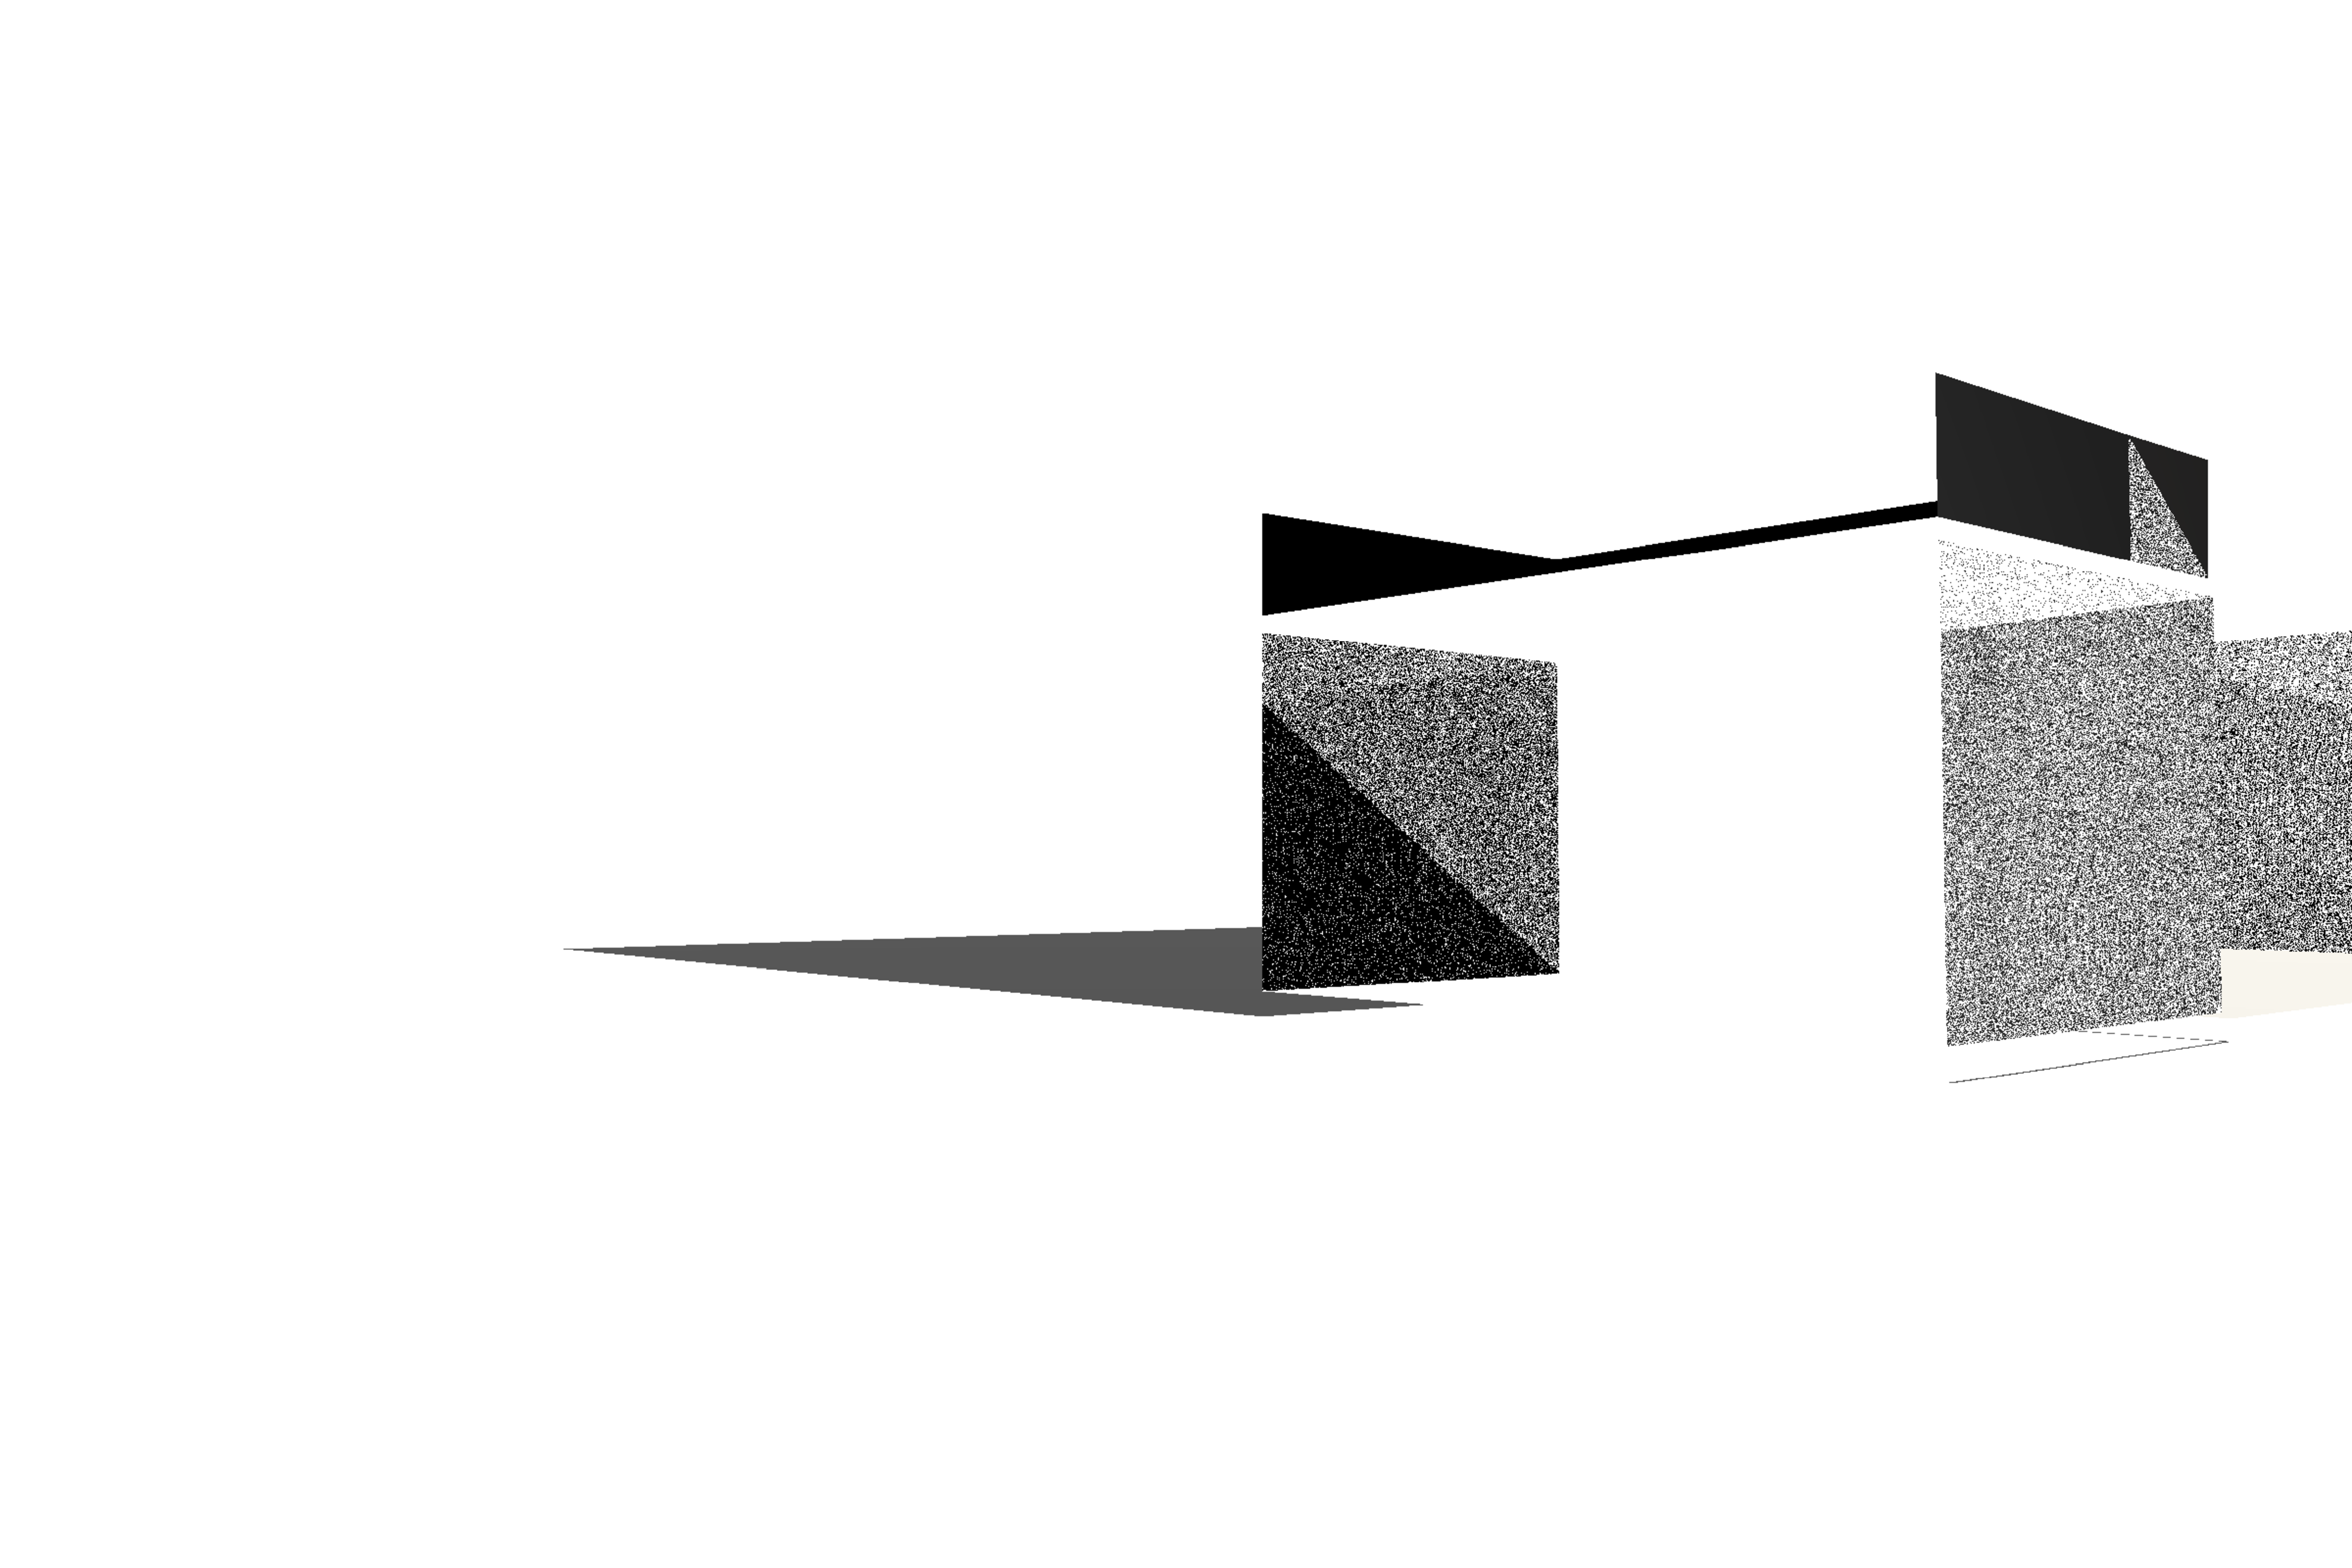
\includegraphics[width=1.5in]{drawings/test_case/results/san_miguel_8_1_light.pdf}%
}
& \hspace{0.1in} &
\fcolorbox{wsu-gray}{white}{%
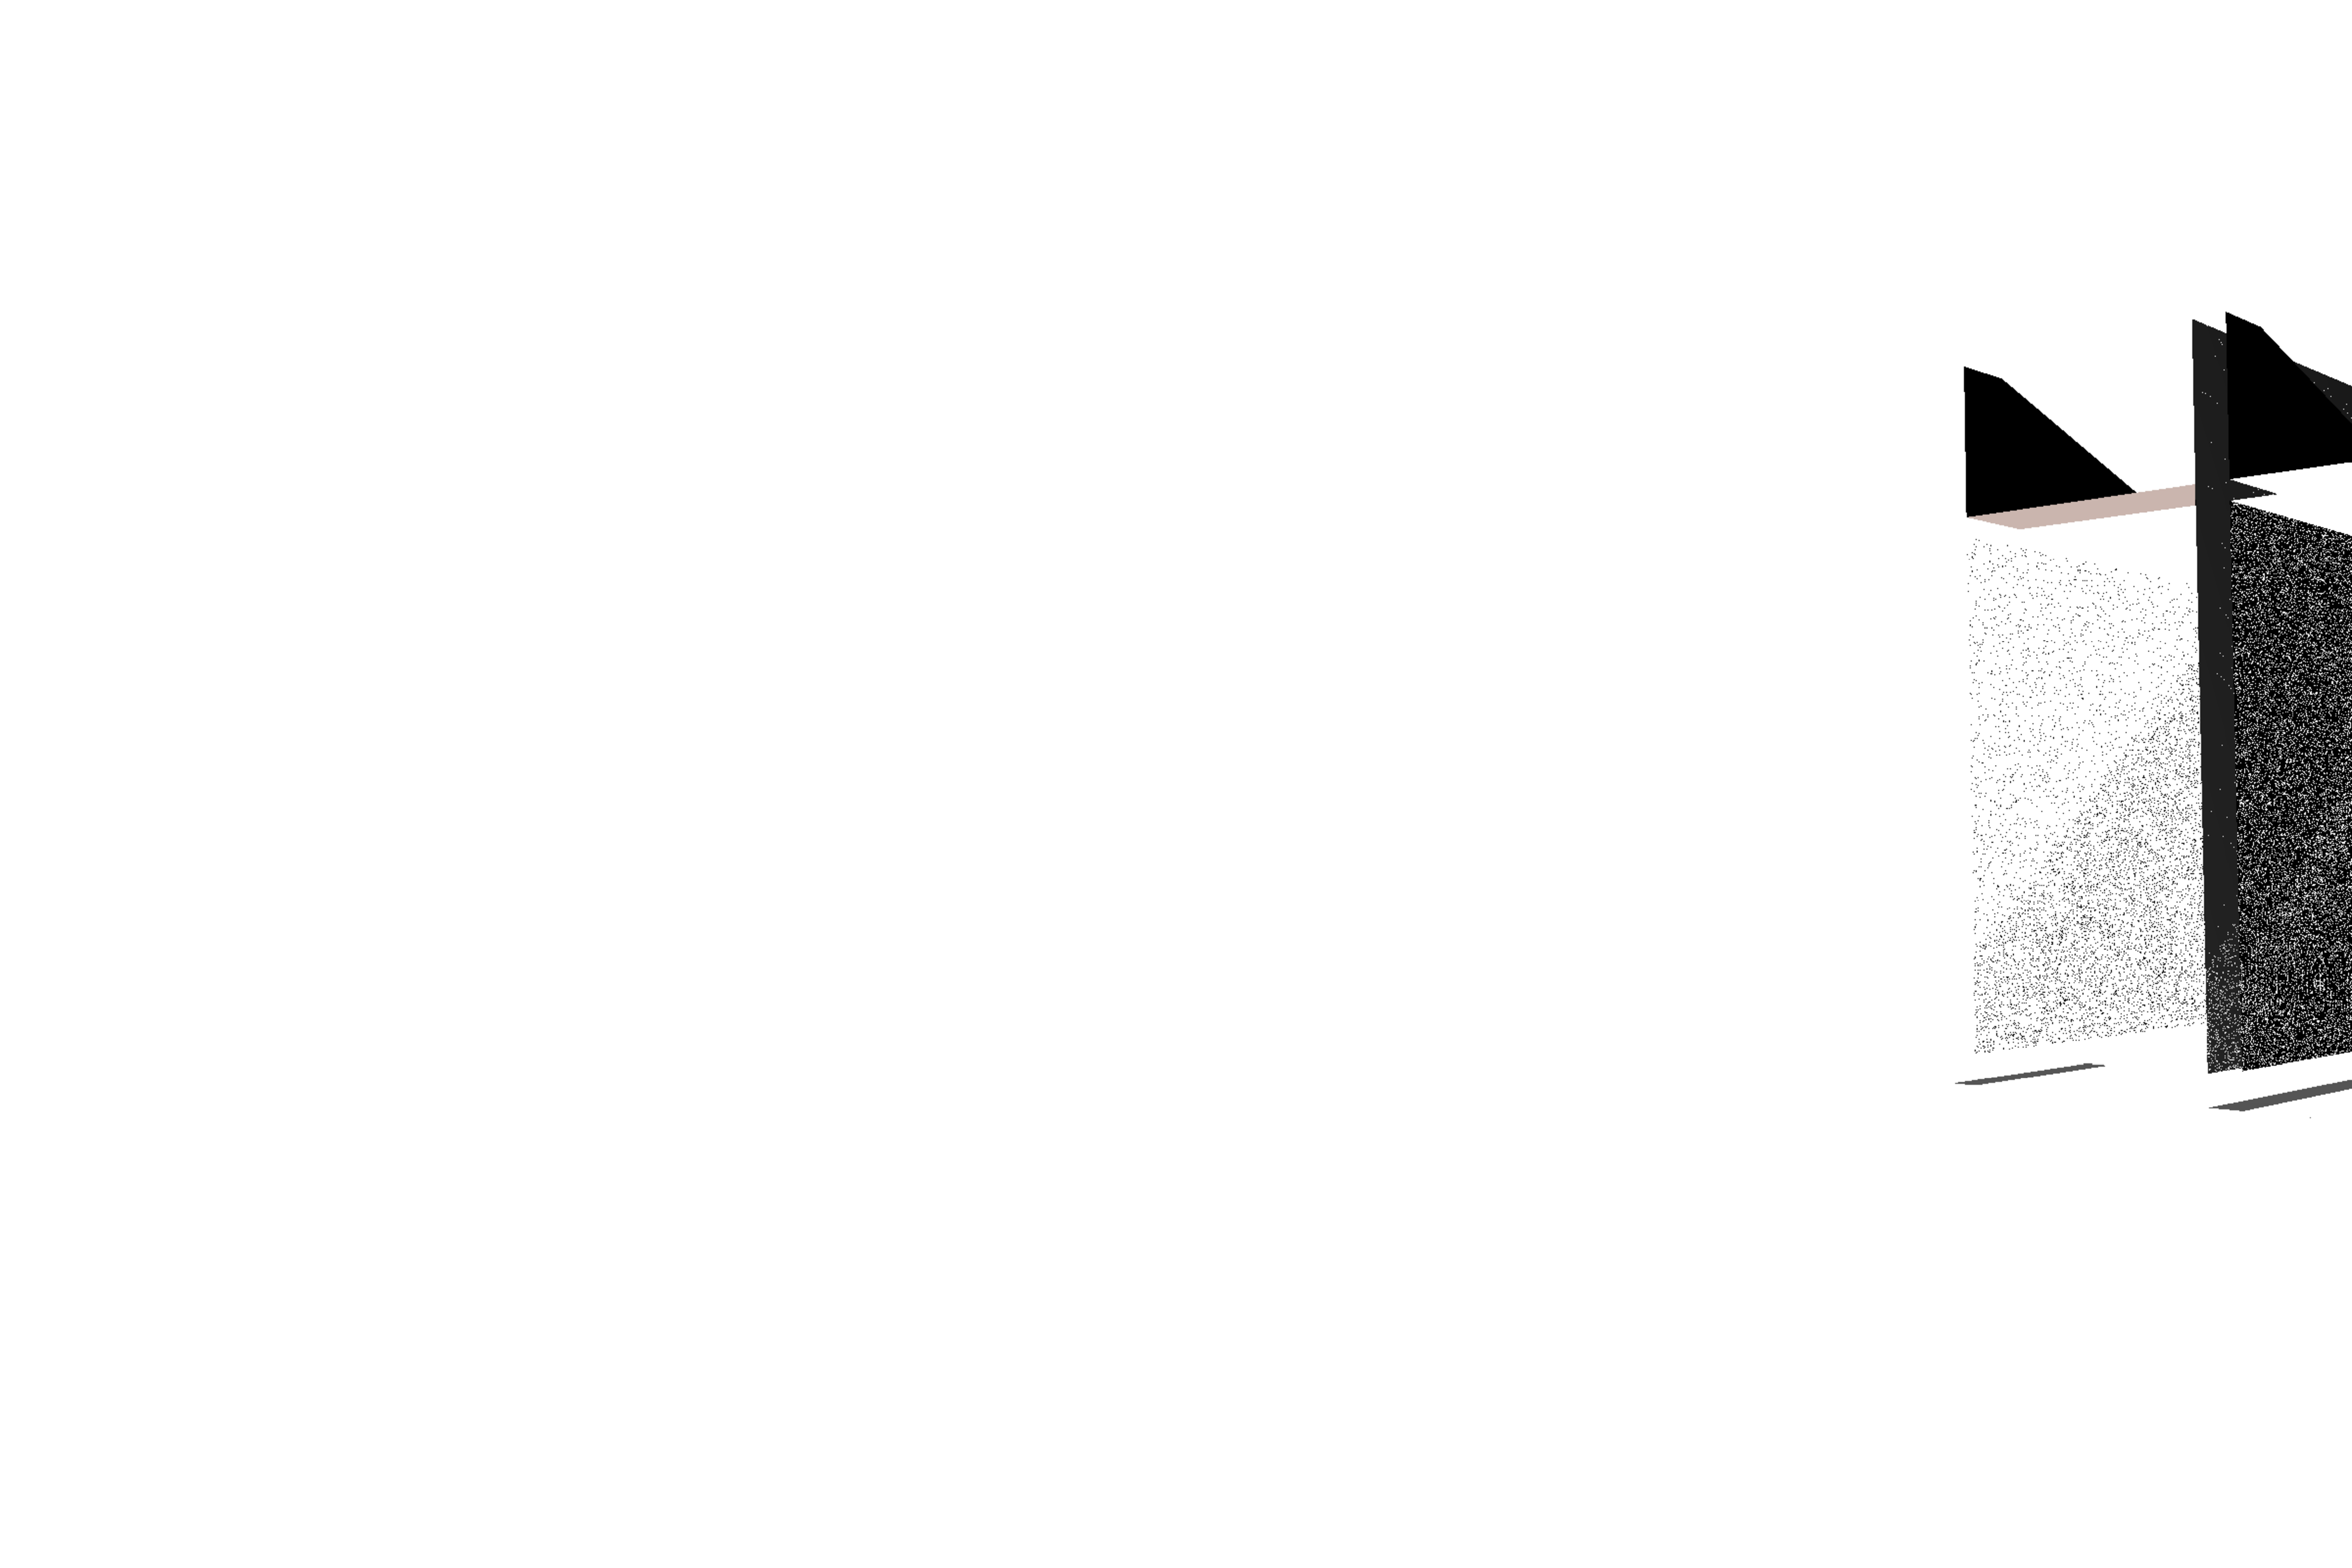
\includegraphics[width=1.5in]{drawings/test_case/results/san_miguel_8_0_light.pdf}%
}
& \hspace{0.1in} &
\fcolorbox{wsu-gray}{white}{%
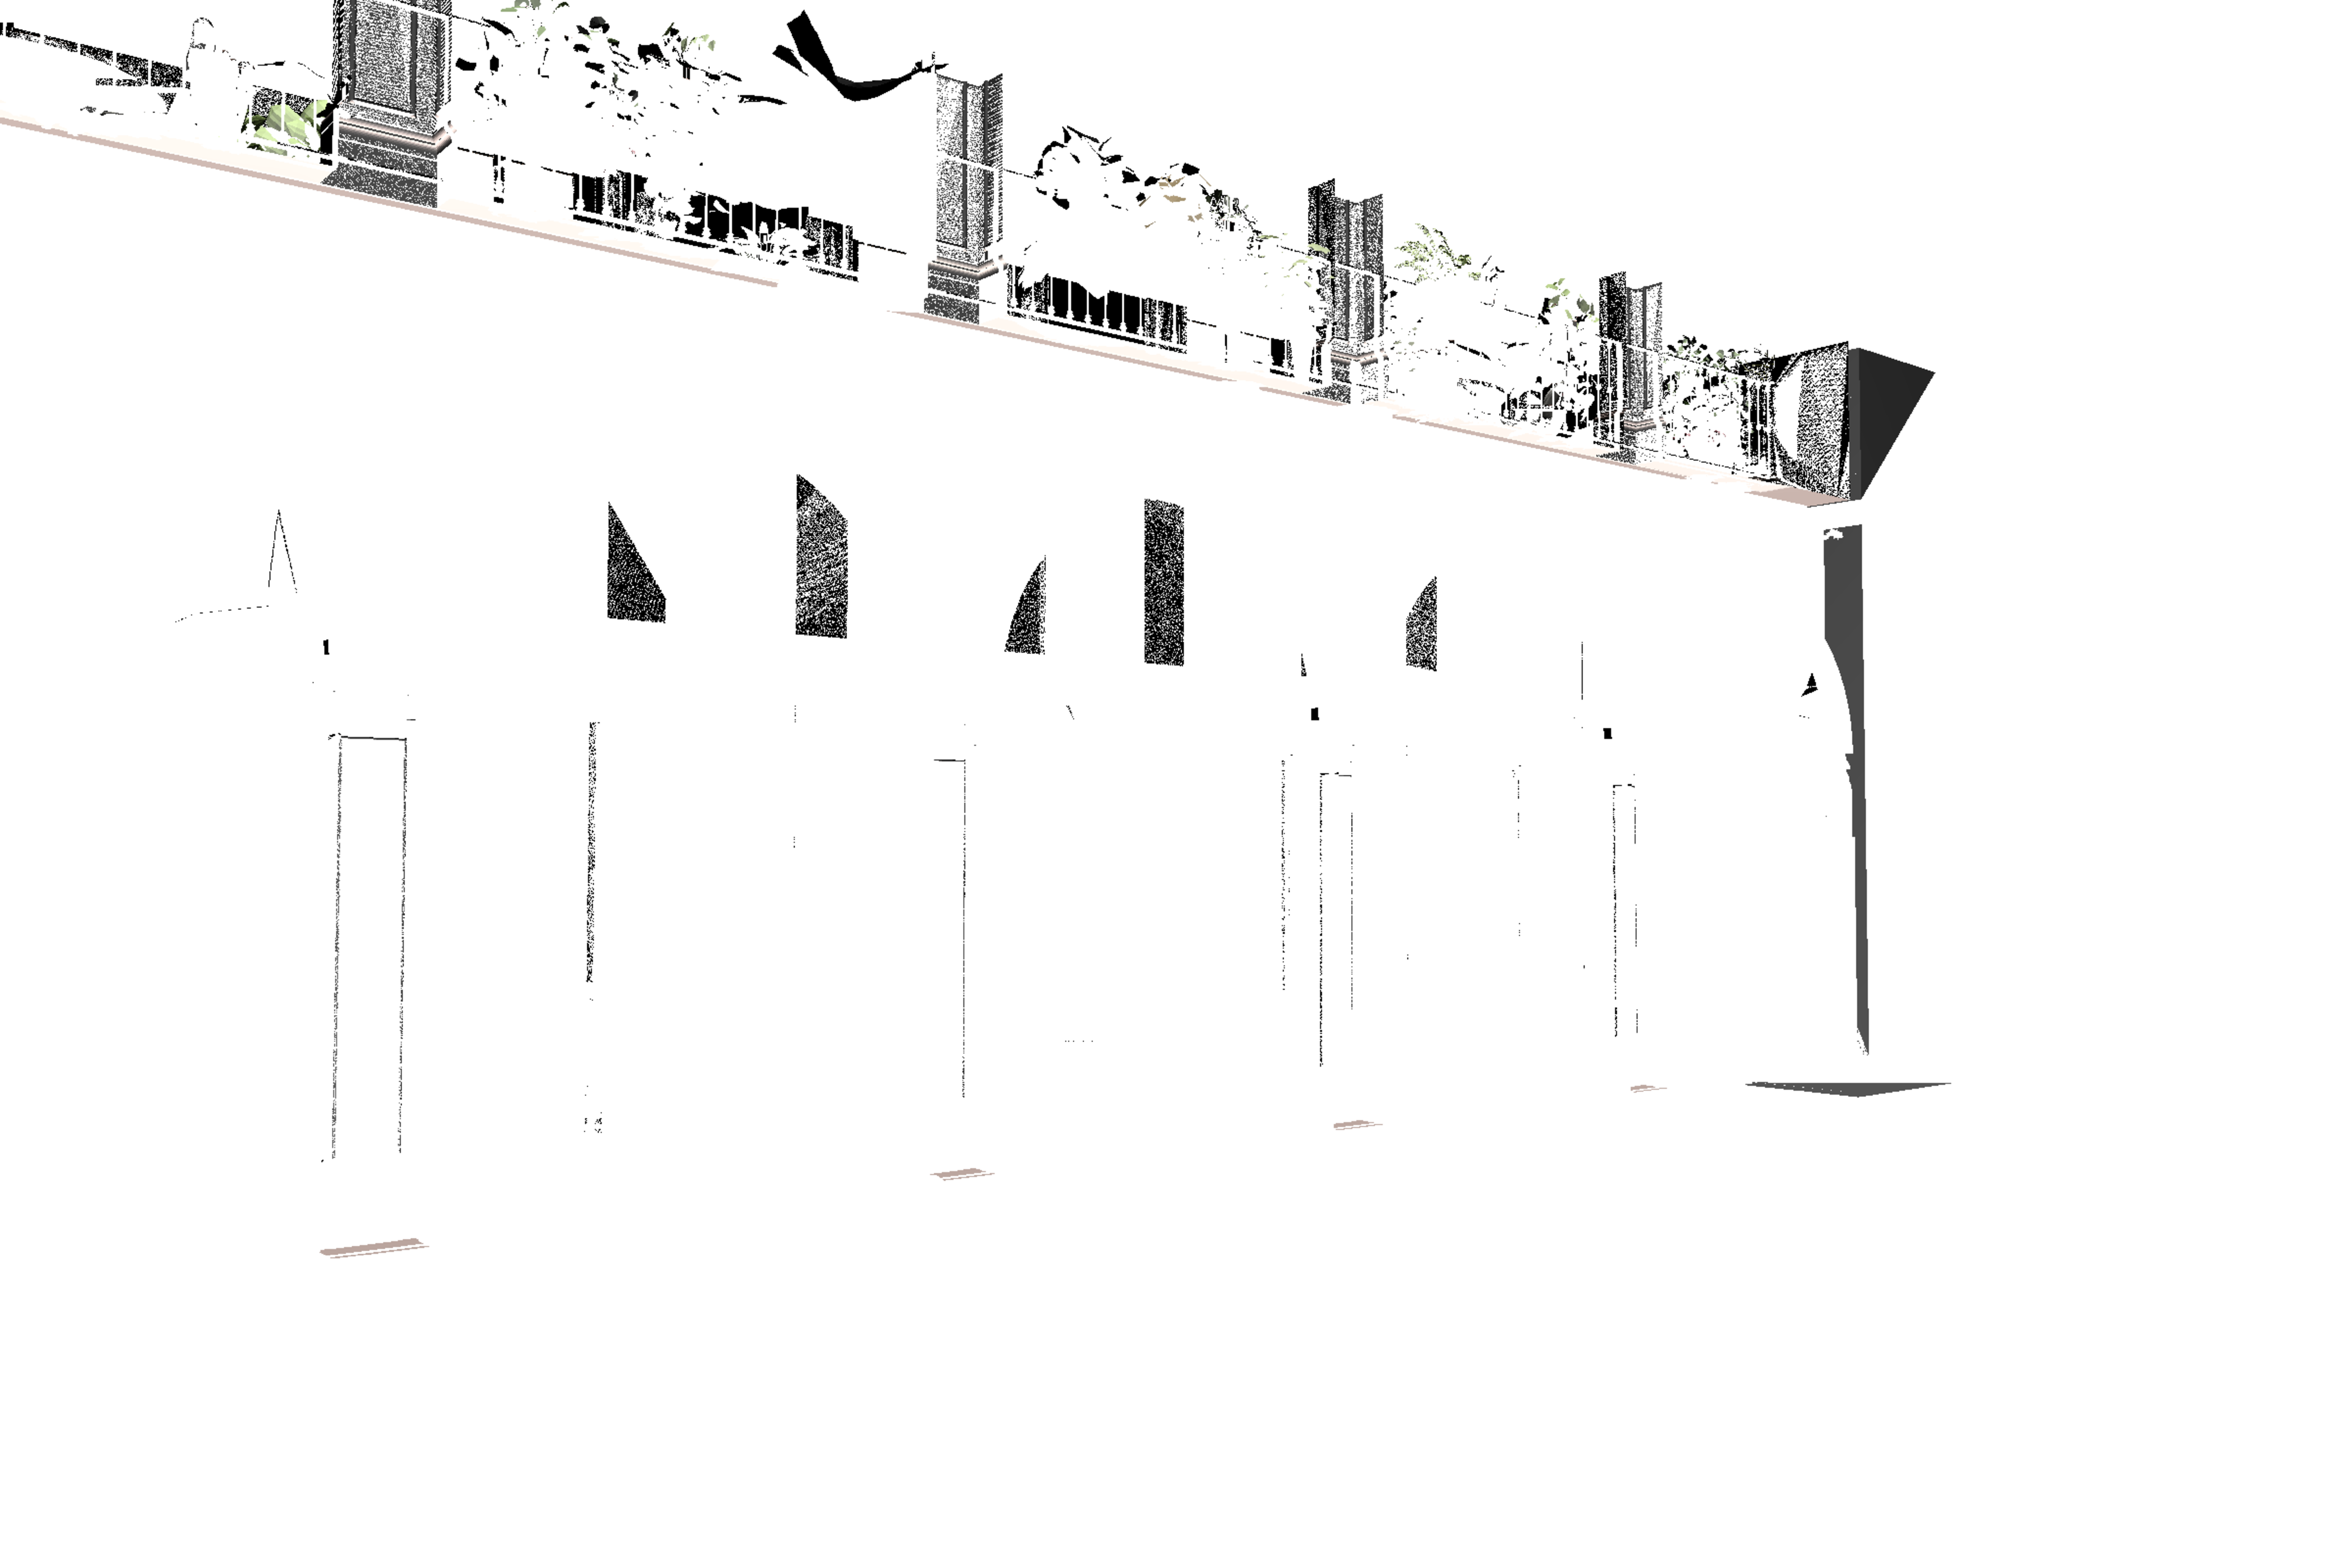
\includegraphics[width=1.5in]{drawings/test_case/results/san_miguel_8_5_light.pdf}%
}
& \hspace{0.1in} &
\fcolorbox{wsu-gray}{white}{%
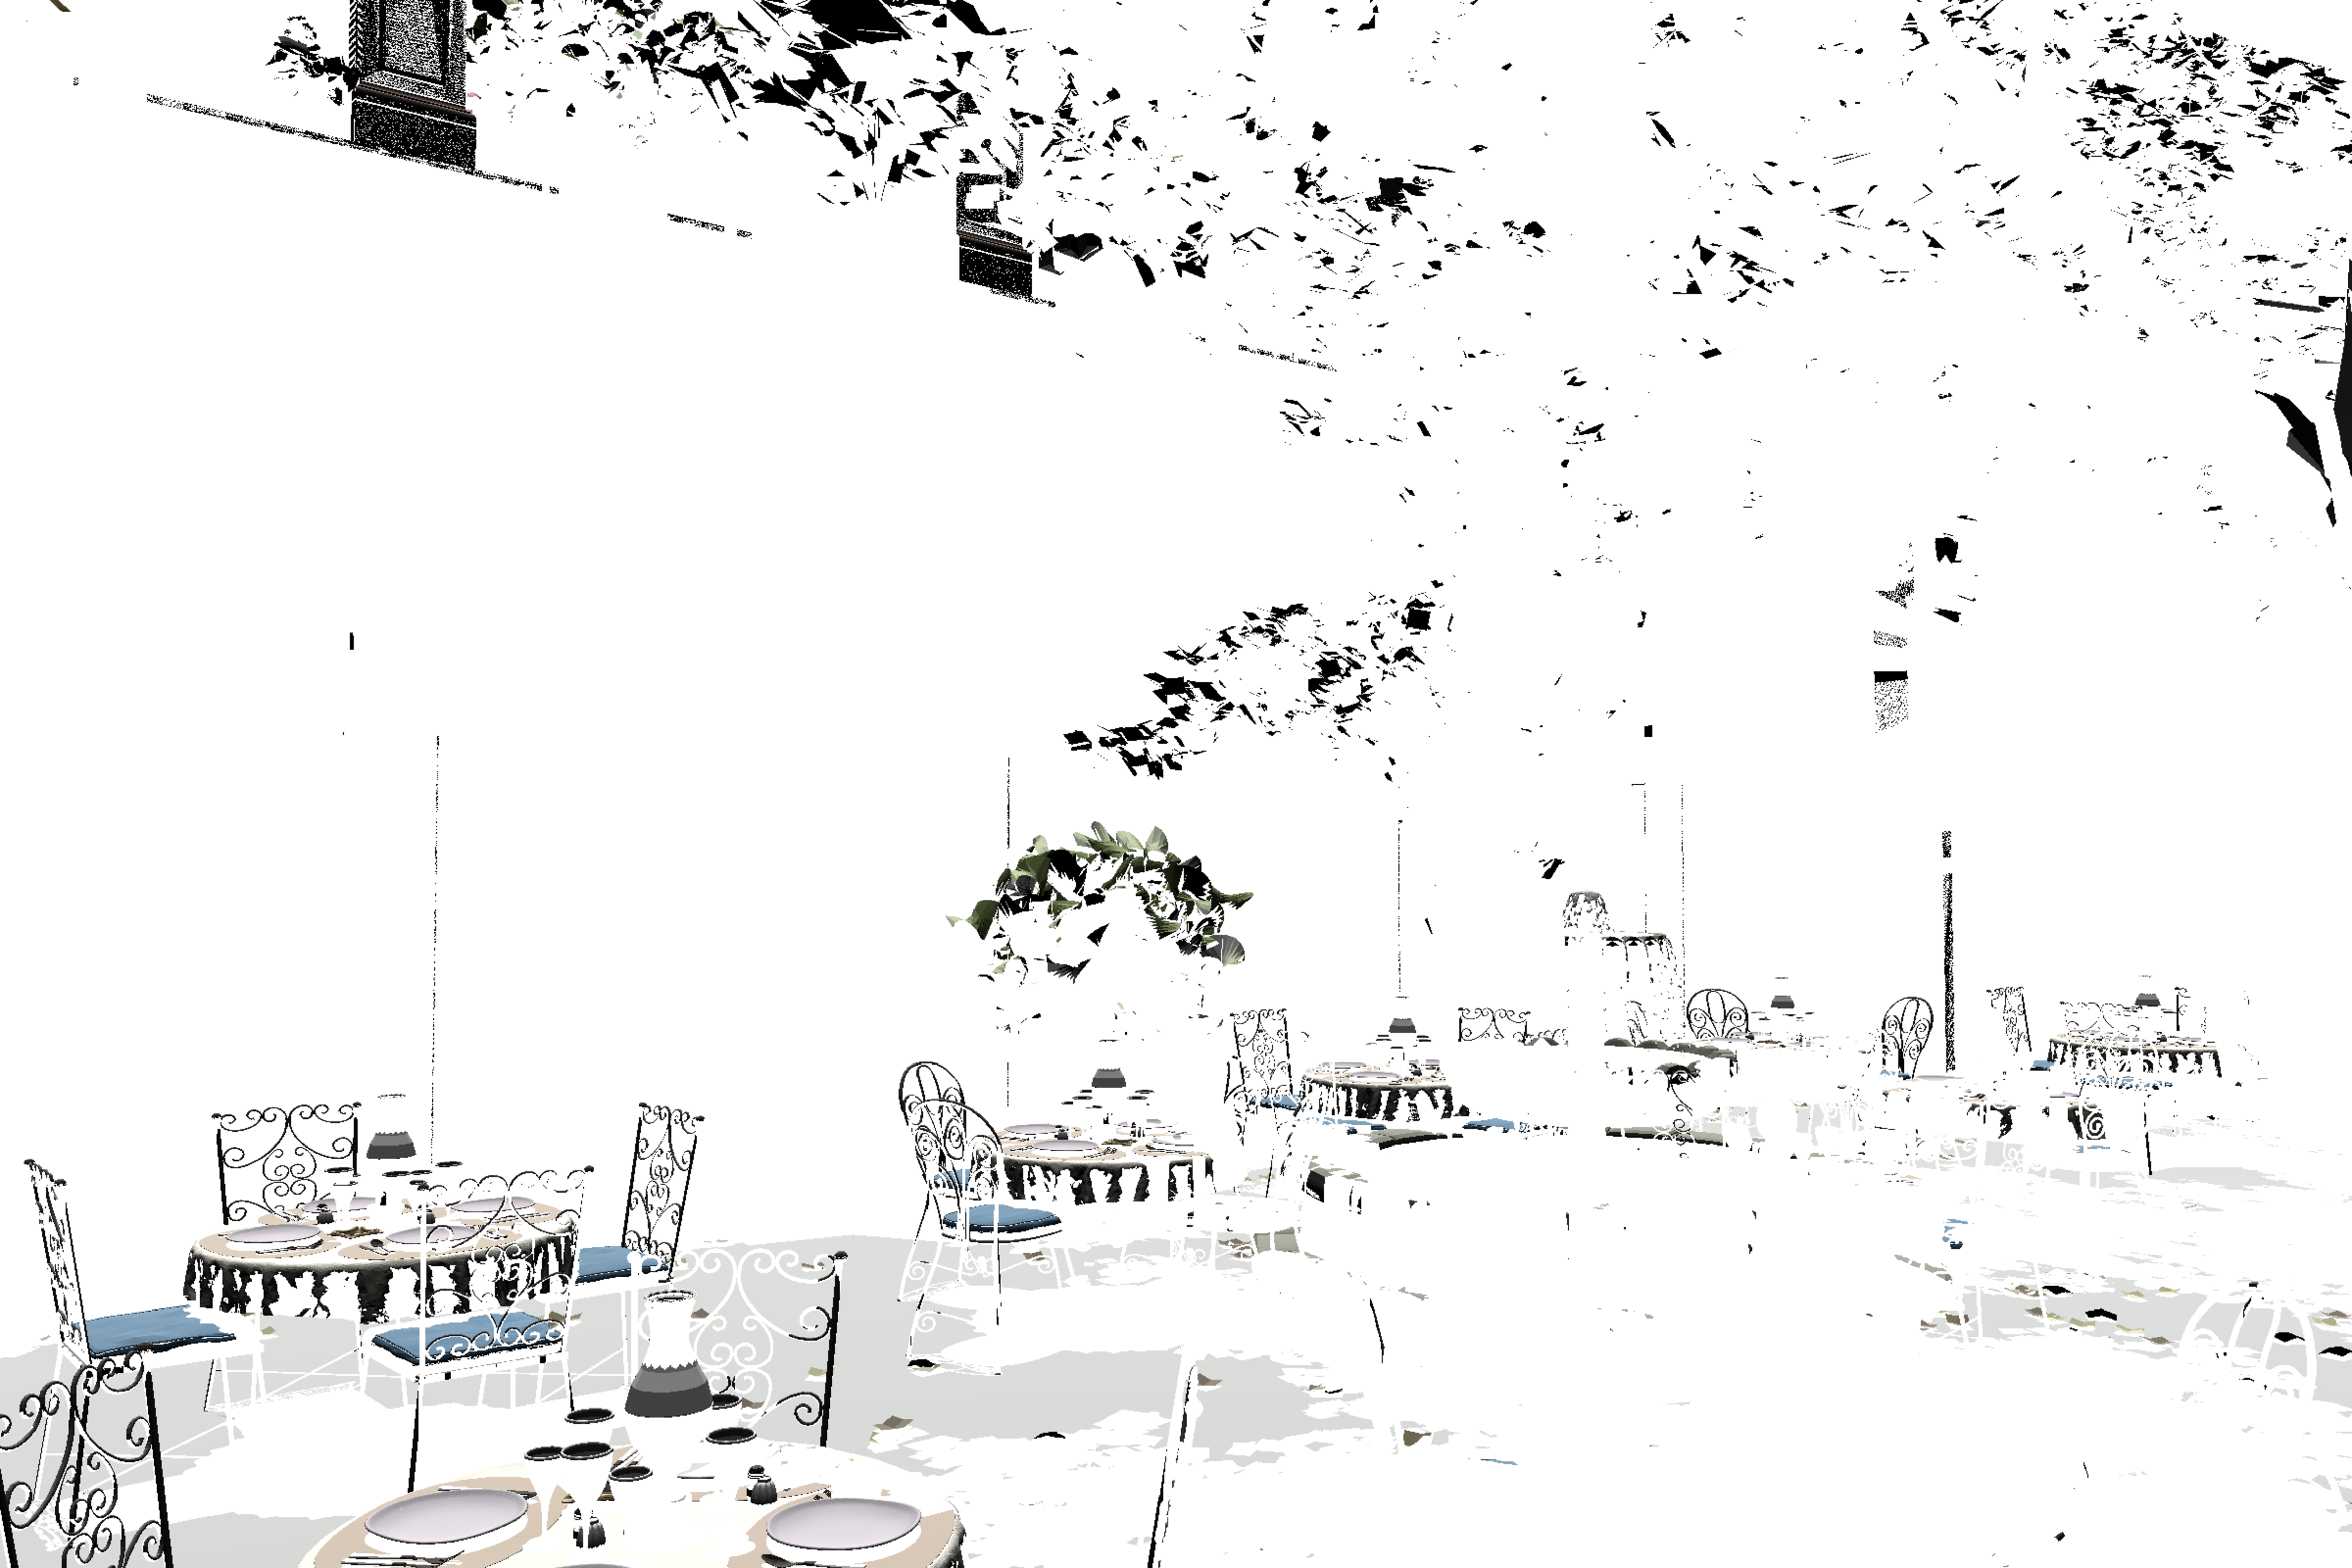
\includegraphics[width=1.5in]{drawings/test_case/results/san_miguel_8_4_light.pdf}%
}
\\
(1, 0, 0) & \hspace{0.1in} & (0, 0, 0) & \hspace{0.1in} &
(1, 0, 1) & \hspace{0.1in} & (0, 0, 1)  \\
\multicolumn{7}{c}{b) Directional Luminaire Traced Image Output} \\
\end{tabular}}
\caption{San Miguel - Traced Image Output from 8-Voxel Test Case}
\label{fig:san-miguel-8-image}
\end{figure}

\newpage

\begin{figure}[!htb]
\setlength\tabcolsep{0pt}
\noindent\makebox[\textwidth]{%
\begin{tabular}{ c c c }
\fcolorbox{wsu-gray}{white}{%
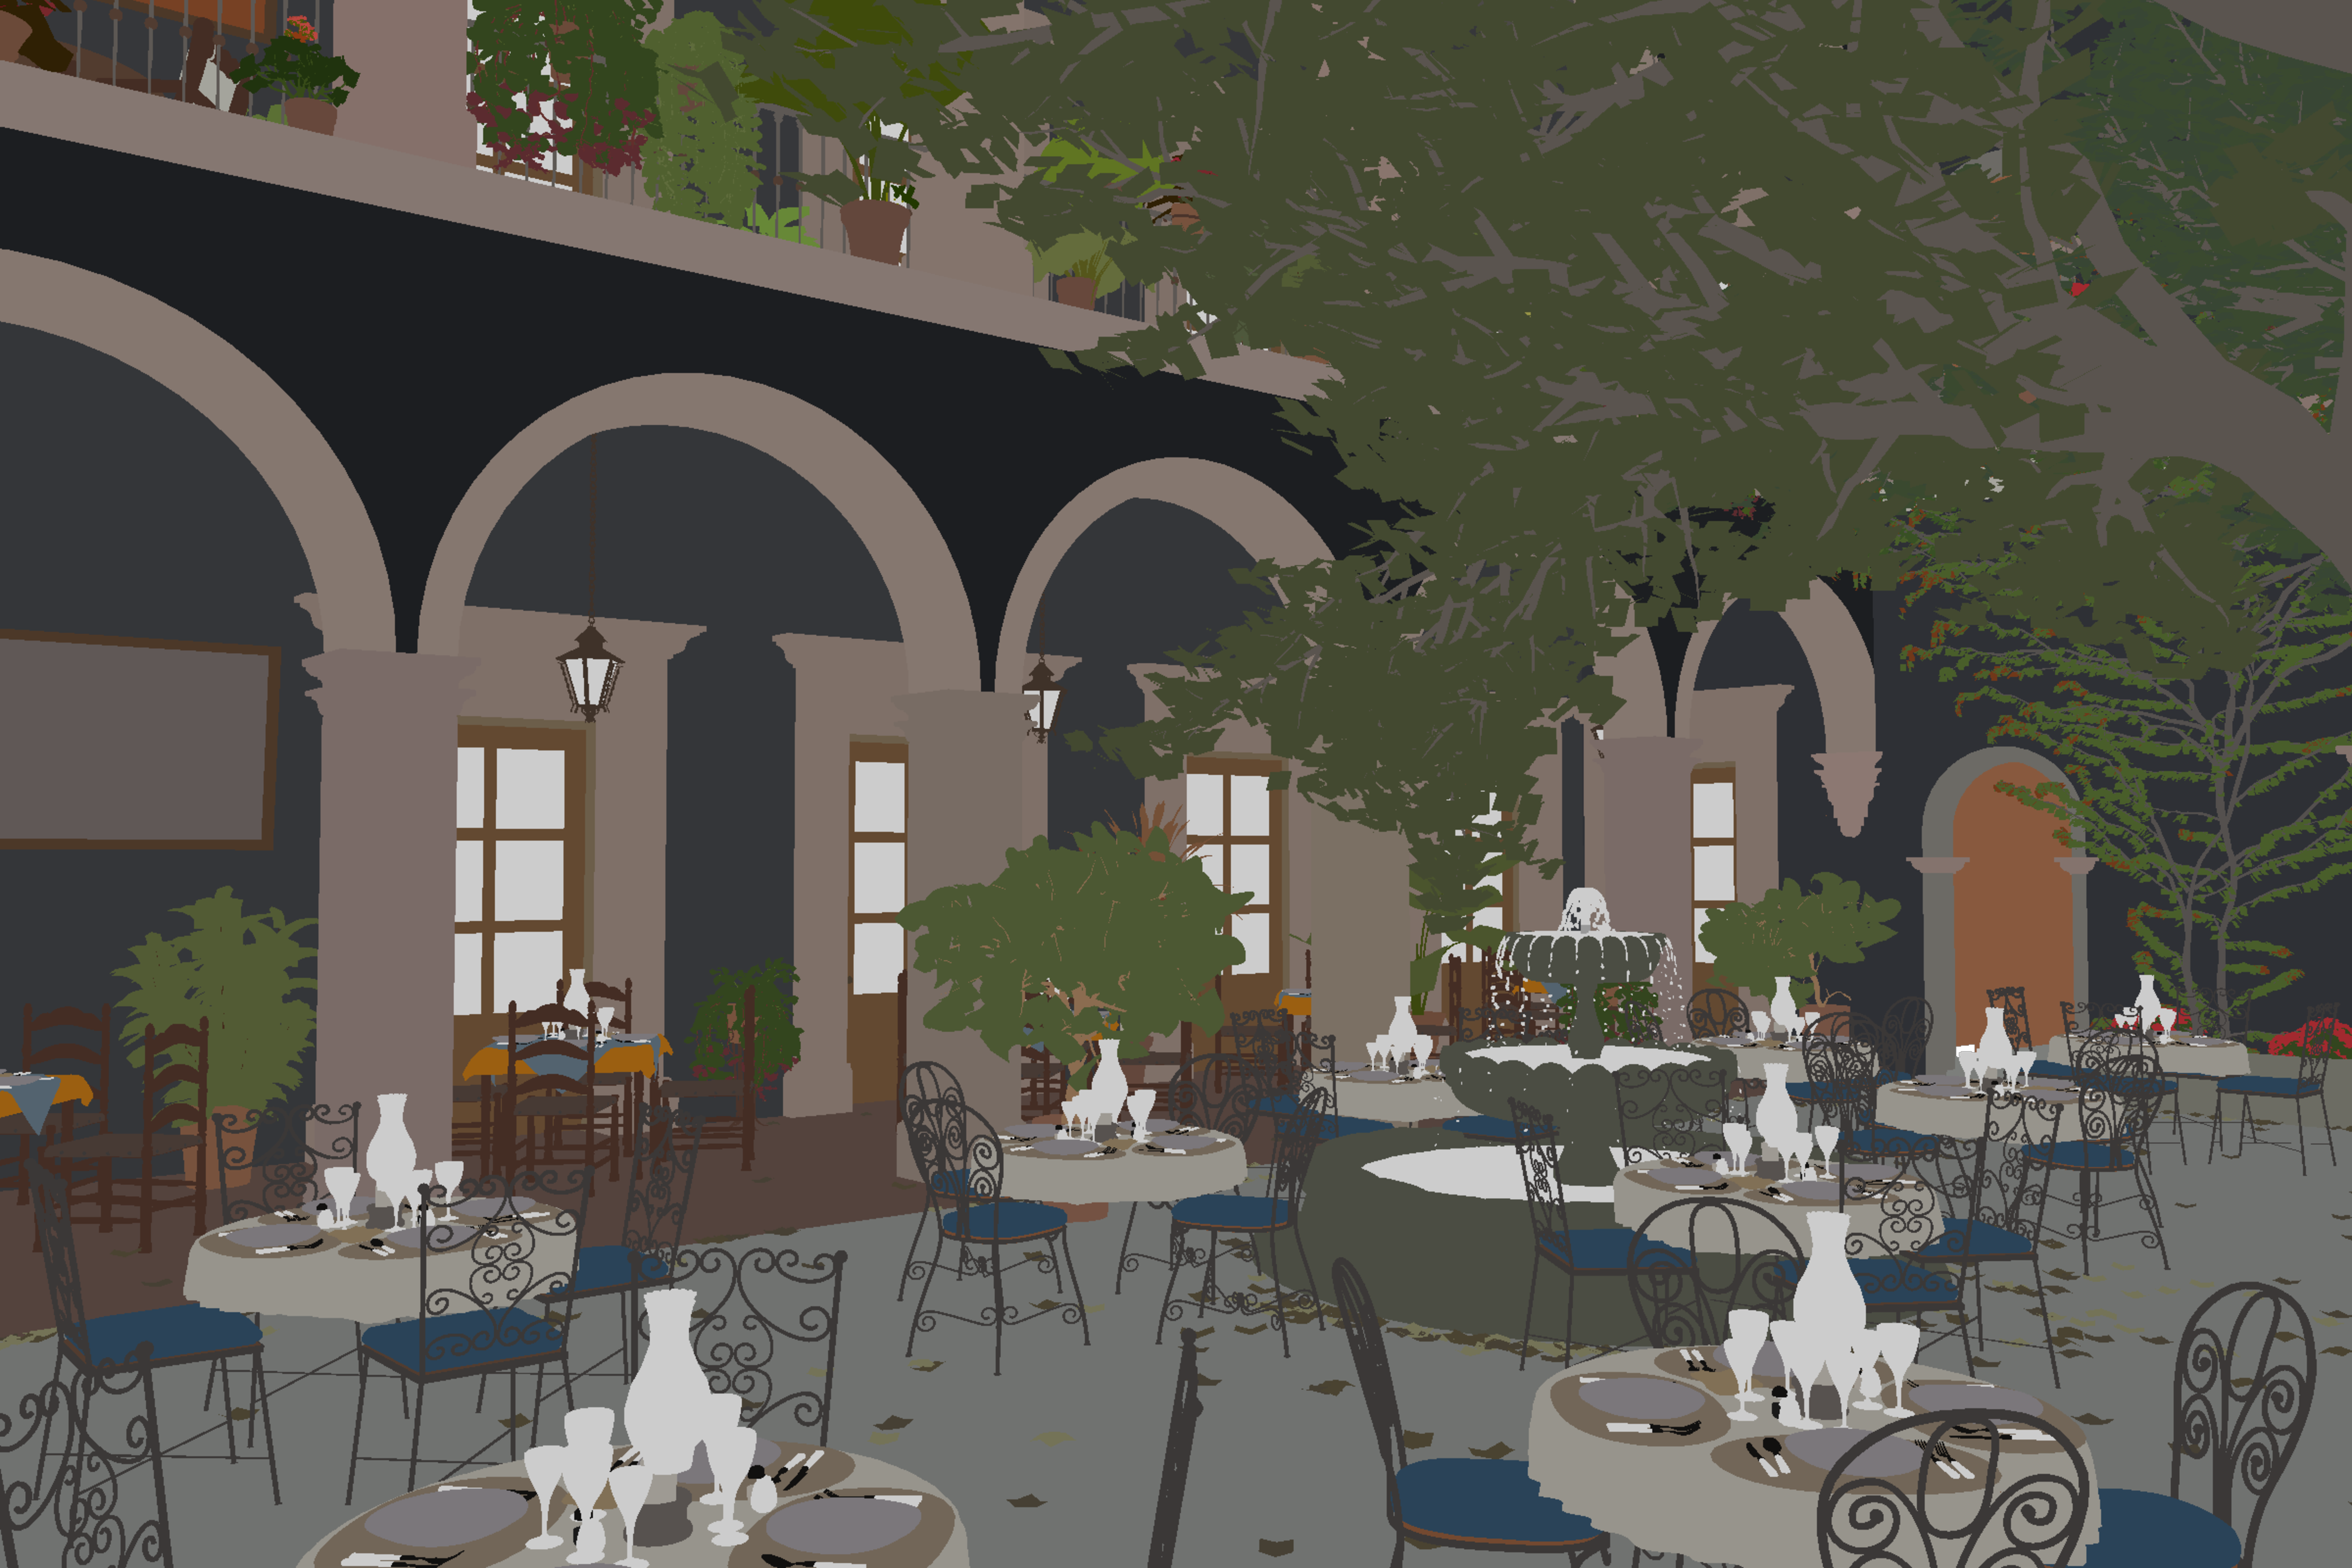
\includegraphics[width=3in]{drawings/test_case/results/analysis/ambient.pdf}%
}
& \hspace{0.1in} &
\fcolorbox{wsu-gray}{white}{%
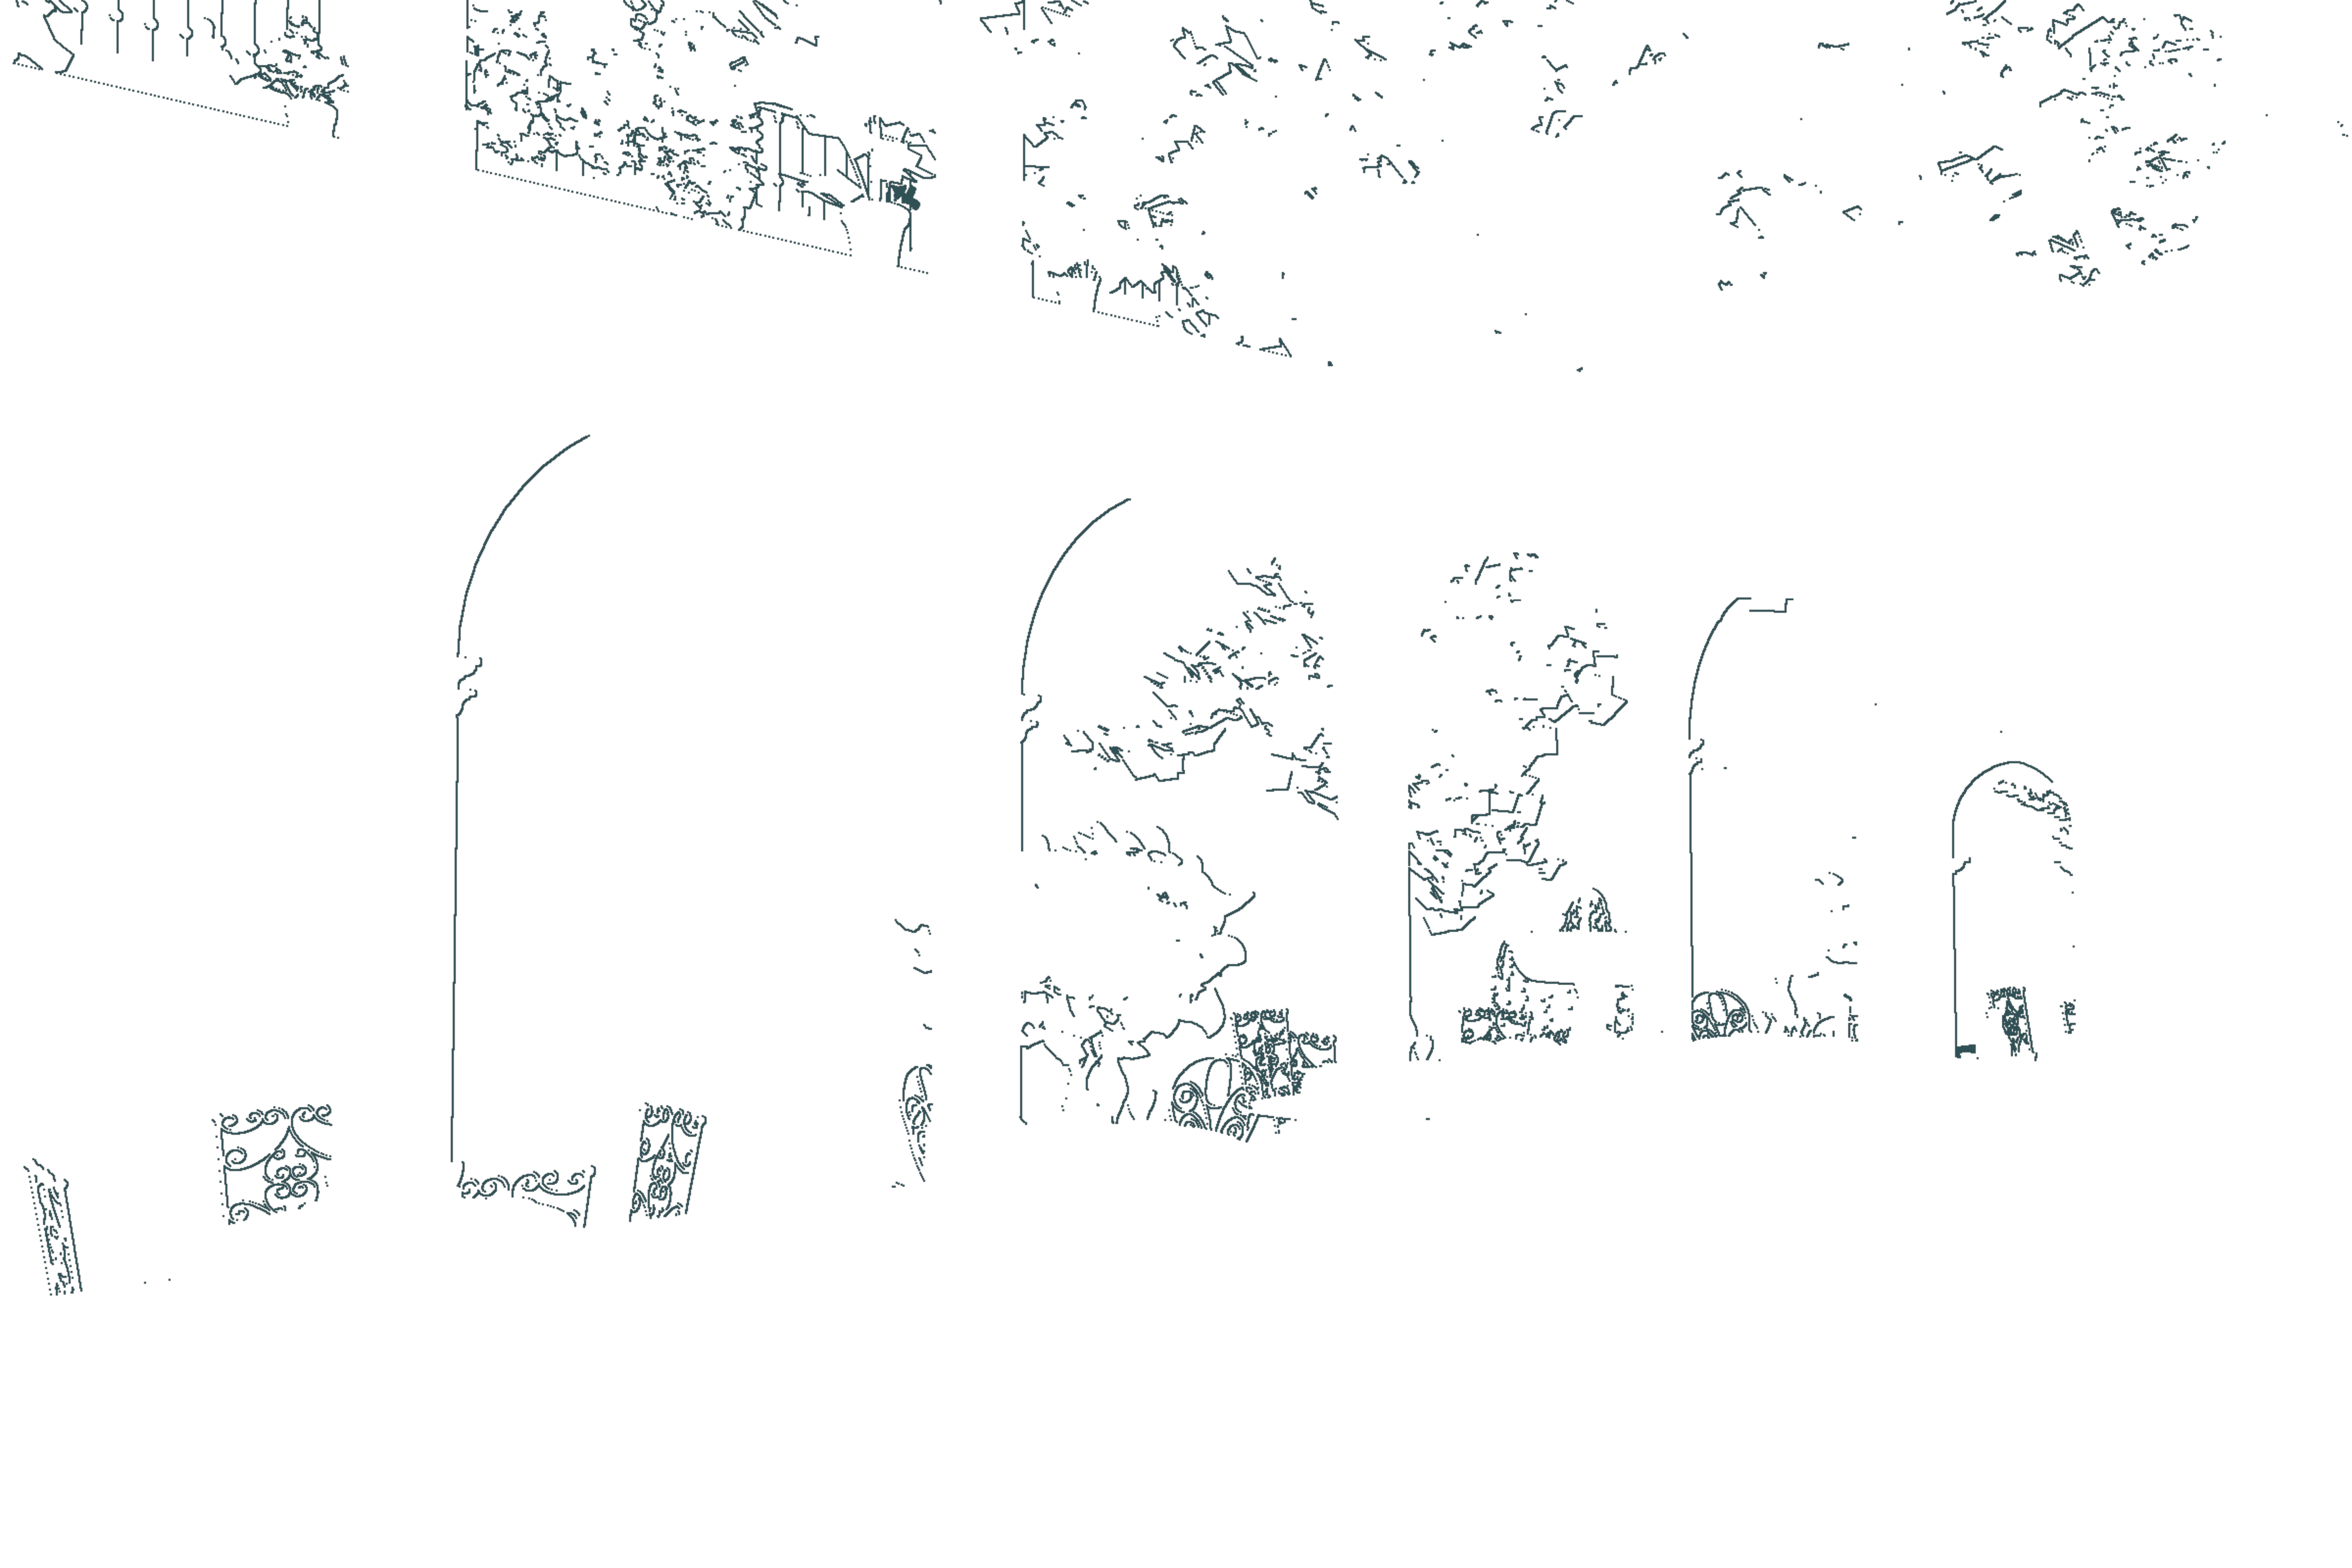
\includegraphics[width=3in]{drawings/test_case/results/analysis/ambient_diff.pdf}%
}
\\
(a) Ambient Light Traced Image & \hspace{0.1in} & (b) Difference from Baseline
\\
\end{tabular}}
\caption{San Miguel - Composited Ambient Image Output for 8-Voxel Test Case}
\label{fig:san-miguel-8}
\end{figure}

Figure~\ref{fig:san-miguel-8}a shows the resulting
image from compositing the ambient traced images. 
Figure~\ref{fig:san-miguel-8}b compares the composited result against the
ambient baseline from Figure~\ref{fig:san-miguel-1}b.  Any non-matching pixel
is set to blue.  This shows us the error introduced from stitching the voxels
together.  As shown in Figure~\ref{fig:ambient_error_graph}, less than 1$\%$
of the total pixels differ from the baseline and most differ by less than 30$\%$.

\begin{figure}[!htb]
\centering
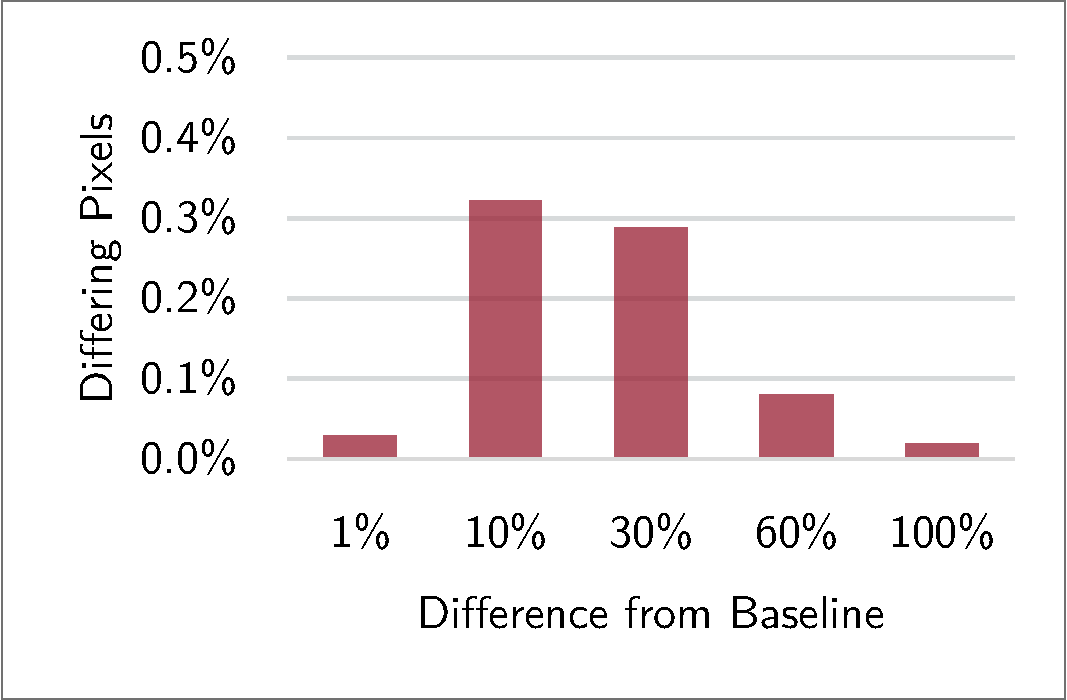
\includegraphics[width=3in]{drawings/test_case/results/analysis/ErrorForAmbient.pdf}
\caption{Difference in Composited 8-Voxel Ambient Traced Images and Baseline}
\label{fig:ambient_error_graph}
\end{figure} 

Figure~\ref{fig:san-miguel-8-composite-0} through
Figure~\ref{fig:san-miguel-8-composite-10000} show the resulting images from
compositing the ambient and directional illuminated images with the indicated
number of light rays.  A comparison image is included in each figure that
compares the result against the baseline from Figure~\ref{fig:san-miguel-1}a. 
Any non-matching pixel is set to red.  Blue pixels indicate differences
resulting from stitching the individual images together.

\begin{figure}[!htb]
\setlength\tabcolsep{0pt}
\noindent\makebox[\textwidth]{%
\begin{tabular}{ c c c }
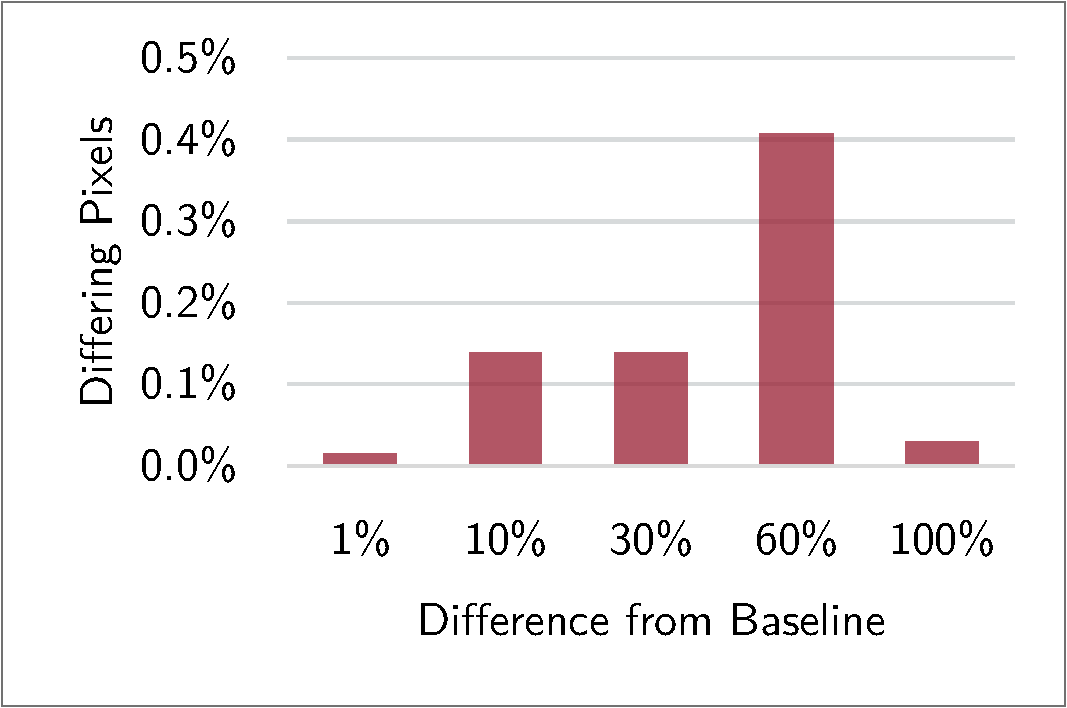
\includegraphics[width=3in]{drawings/test_case/results/analysis/ErrorFor0.pdf}
& \hspace{0.1in} &
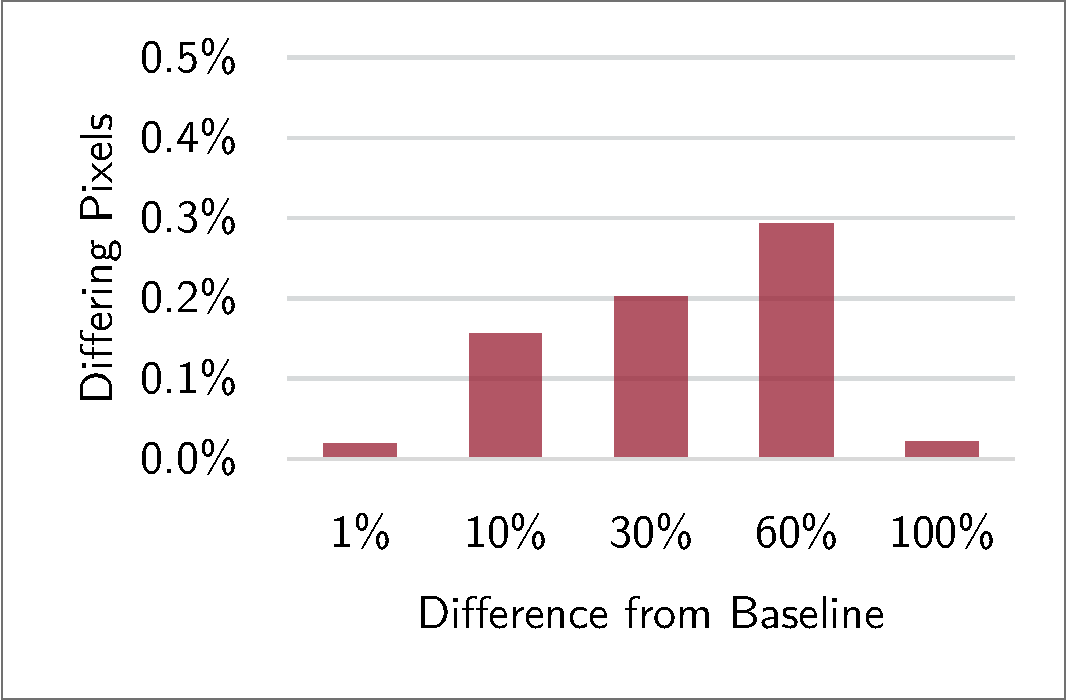
\includegraphics[width=3in]{drawings/test_case/results/analysis/ErrorFor100.pdf}
\\
(a) No Shadow Mesh & \hspace{0.1in} & (b) 100$^2$ \\
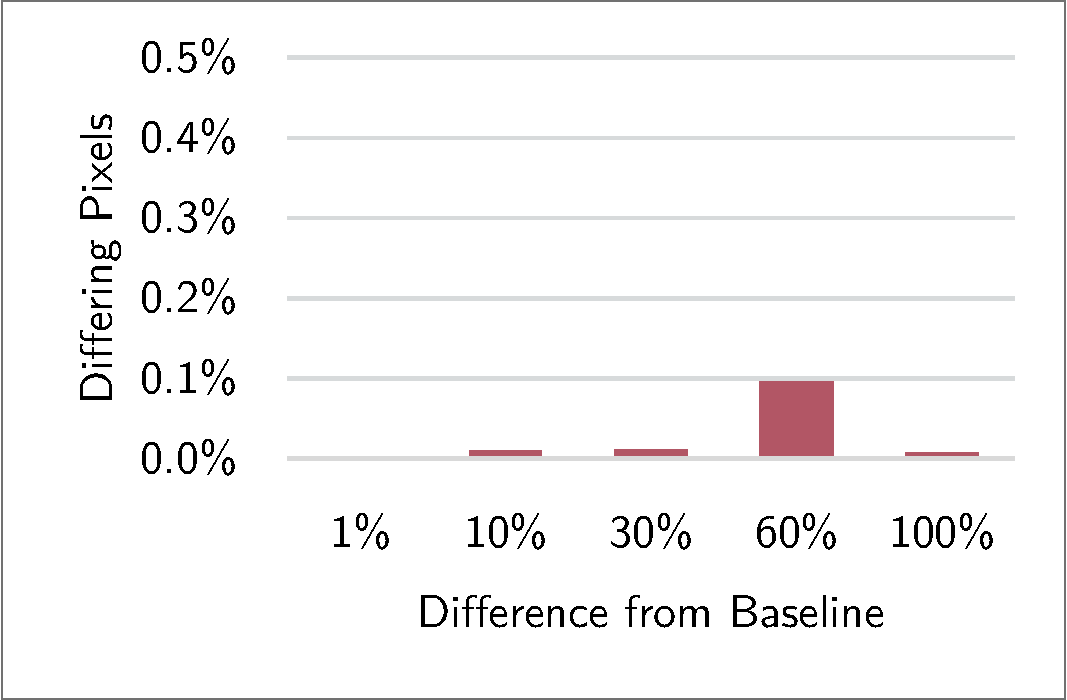
\includegraphics[width=3in]{drawings/test_case/results/analysis/ErrorFor1000.pdf}
& \hspace{0.1in} &
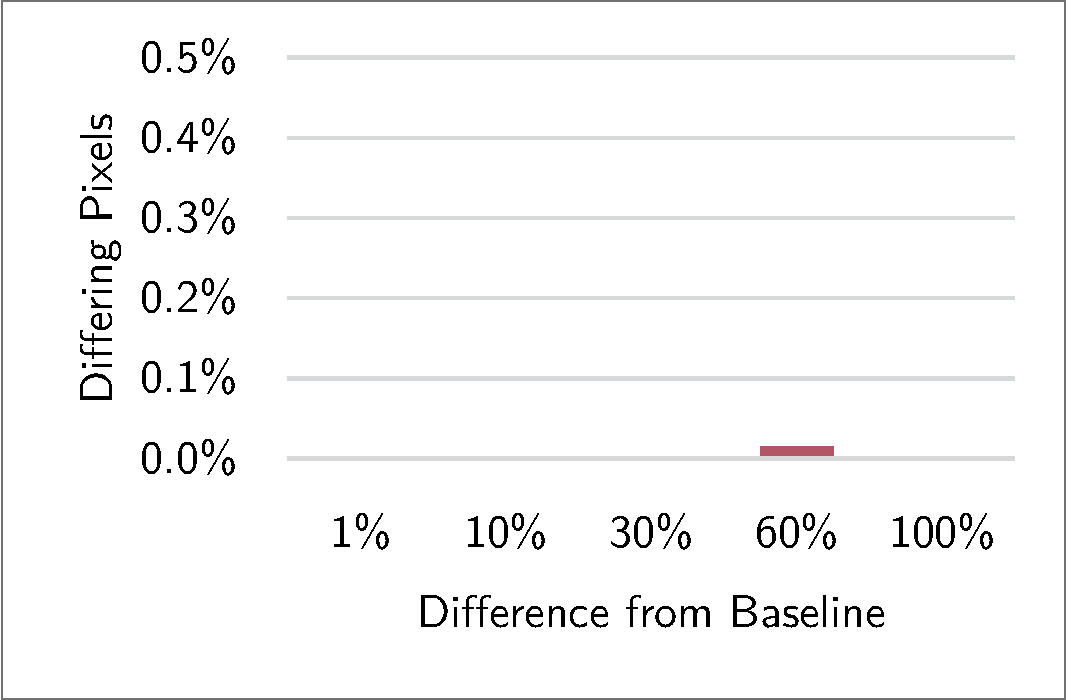
\includegraphics[width=3in]{drawings/test_case/results/analysis/ErrorFor10000.pdf}
\\
(c) 1000$^2$ & \hspace{0.1in} & (d) 10000$^2$ 
\end{tabular}}
\caption{Difference in Composited 8-Voxel Traced Images and Baseline}
\label{fig:light_error_graph}
\end{figure}

From Figure~\ref{fig:light_error_graph} we can see that with a sufficiently
sized shadow mesh we can produce a quality image using our algorithm.  A shadow
mesh with a resolution of 100$^2$ only slightly improves the final image,
reducing the number of pixels with an error from 0.74$\%$ to 0.69$\%$. 
Increasing the resolution to 1000$^2$ reduces the error to 0.13$\%$ and
increasing to 10000$^2$ reducing the error to just 0.02$\%$.  As the
resolution of the shadow mesh increases so does the time to compute it.  We
analyze the performance of the algorithm in the next section. 

\begin{figure}
\setlength\tabcolsep{0pt}
\noindent\makebox[\textwidth]{%
\begin{tabular}{ c }
\fcolorbox{wsu-gray}{white}{%
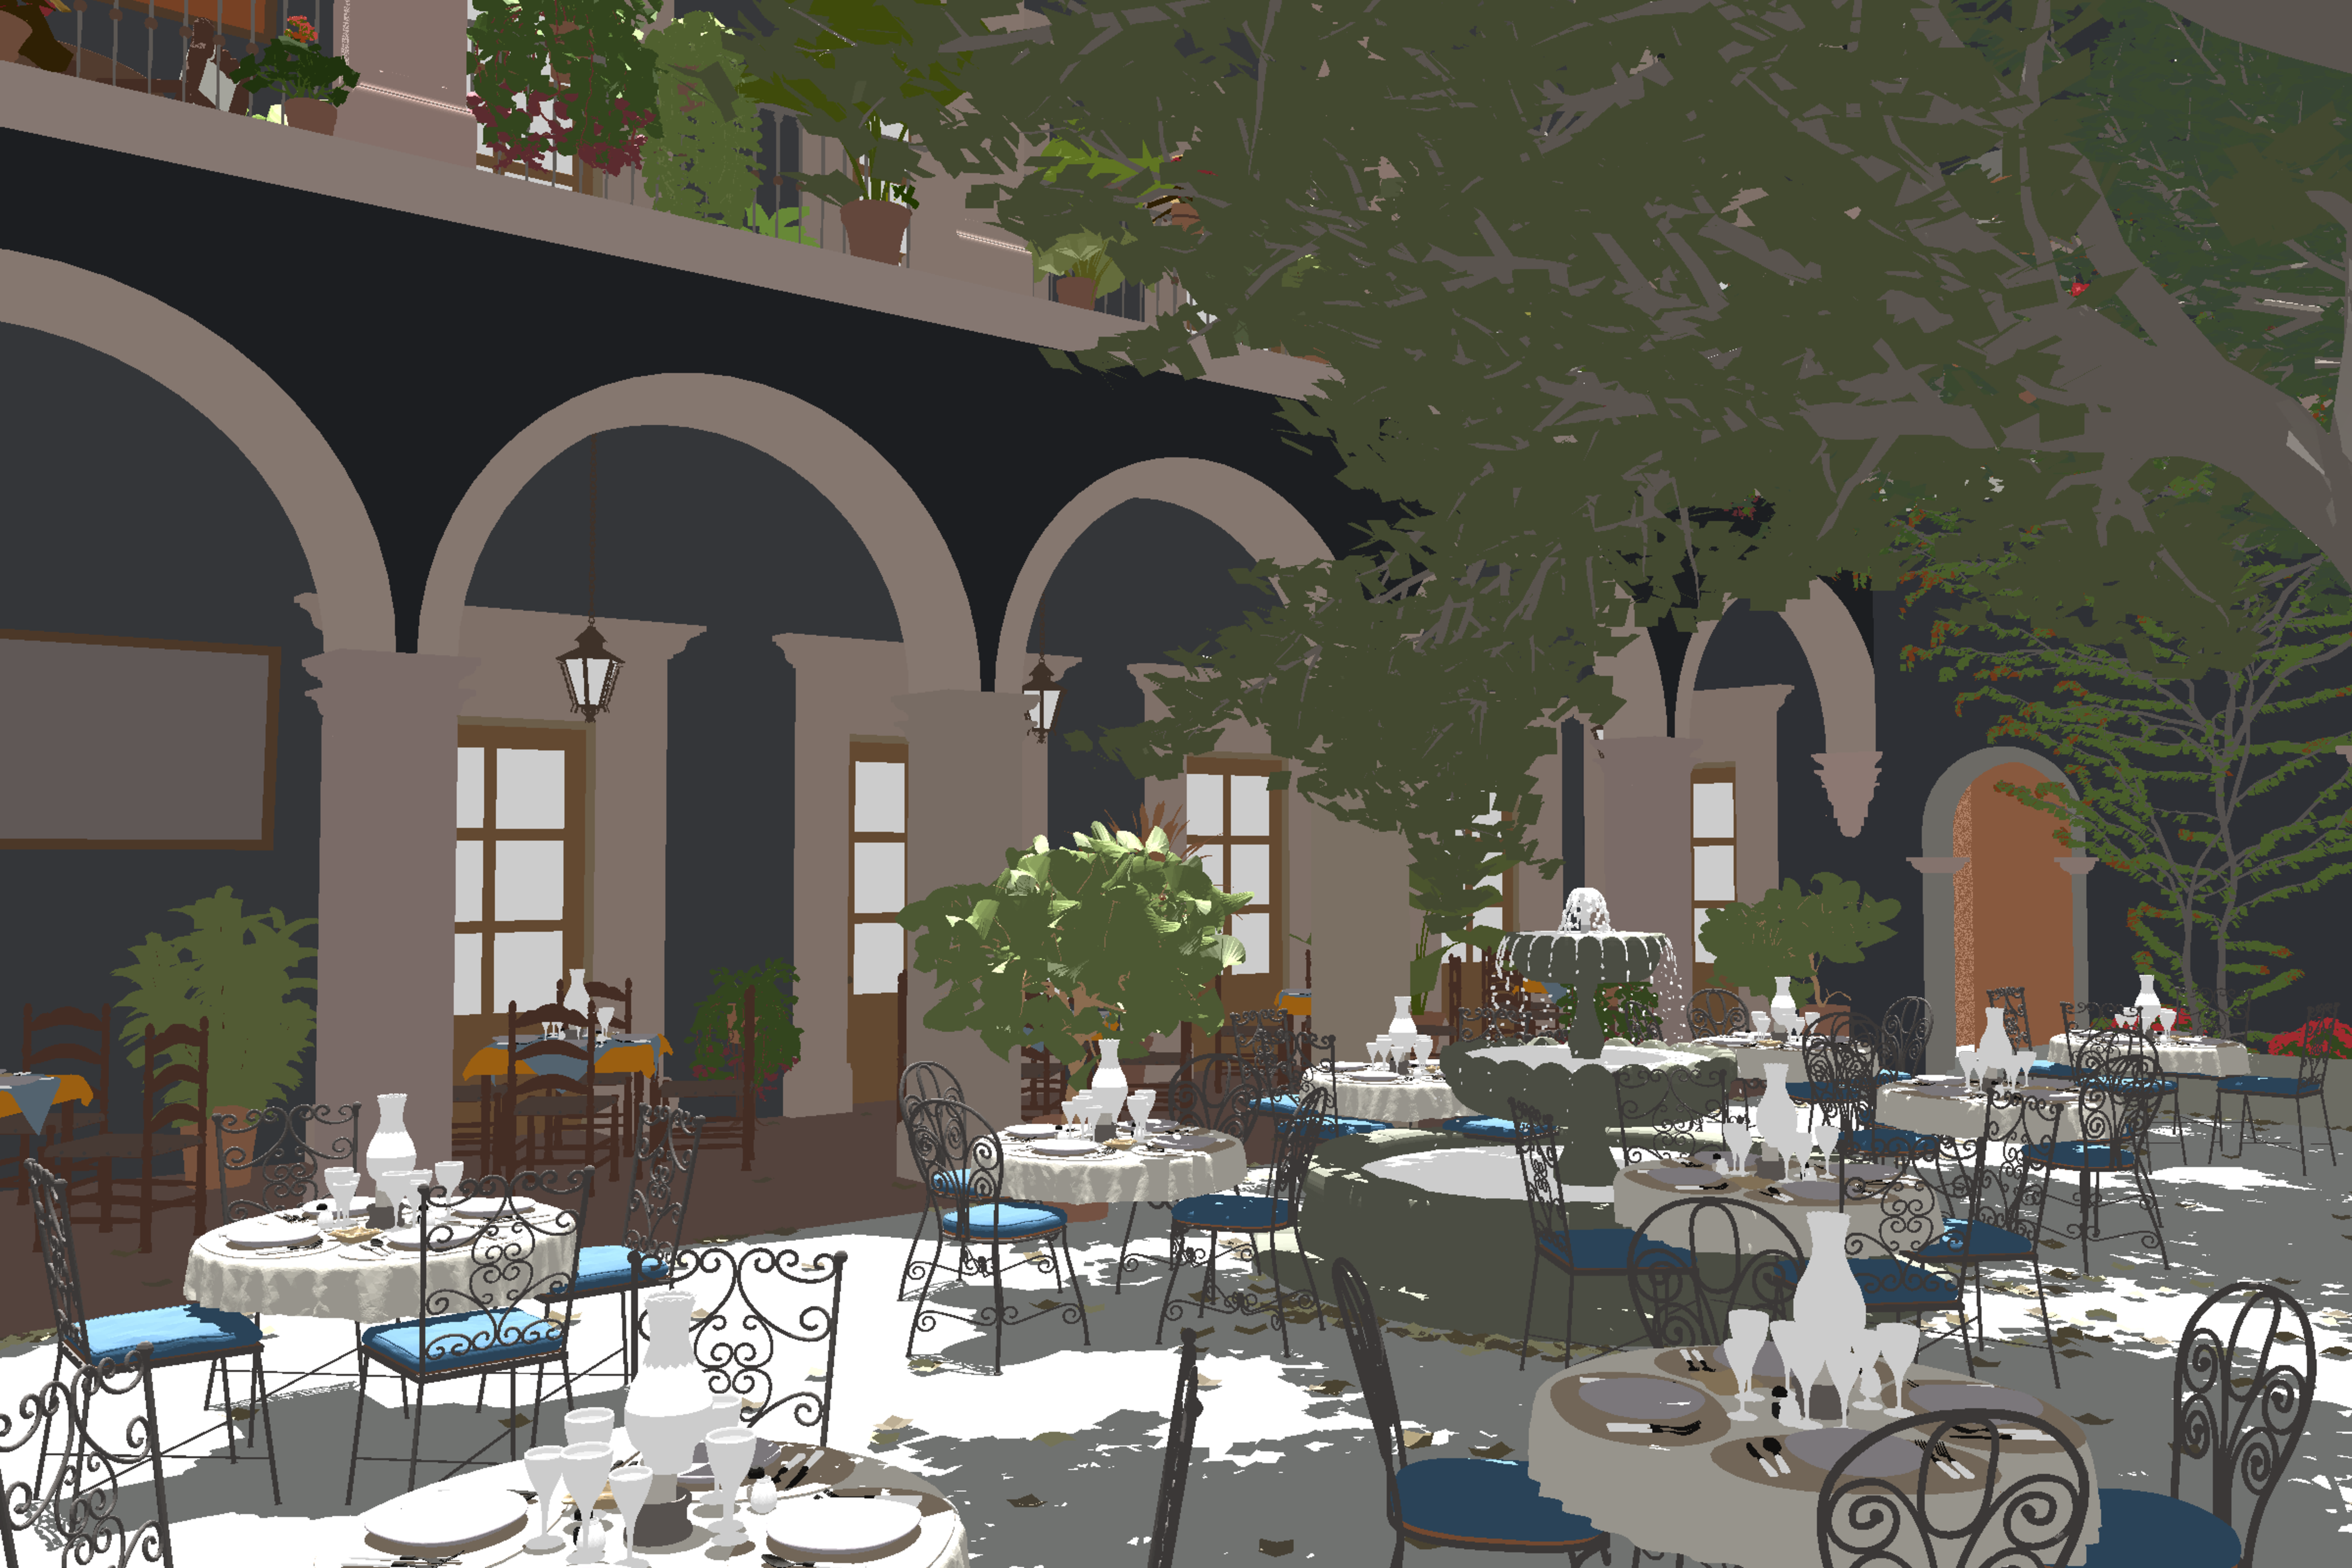
\includegraphics[width=6in]{drawings/test_case/results/analysis/image_8_shadow_0.pdf}%
} \\
\fcolorbox{wsu-gray}{white}{%
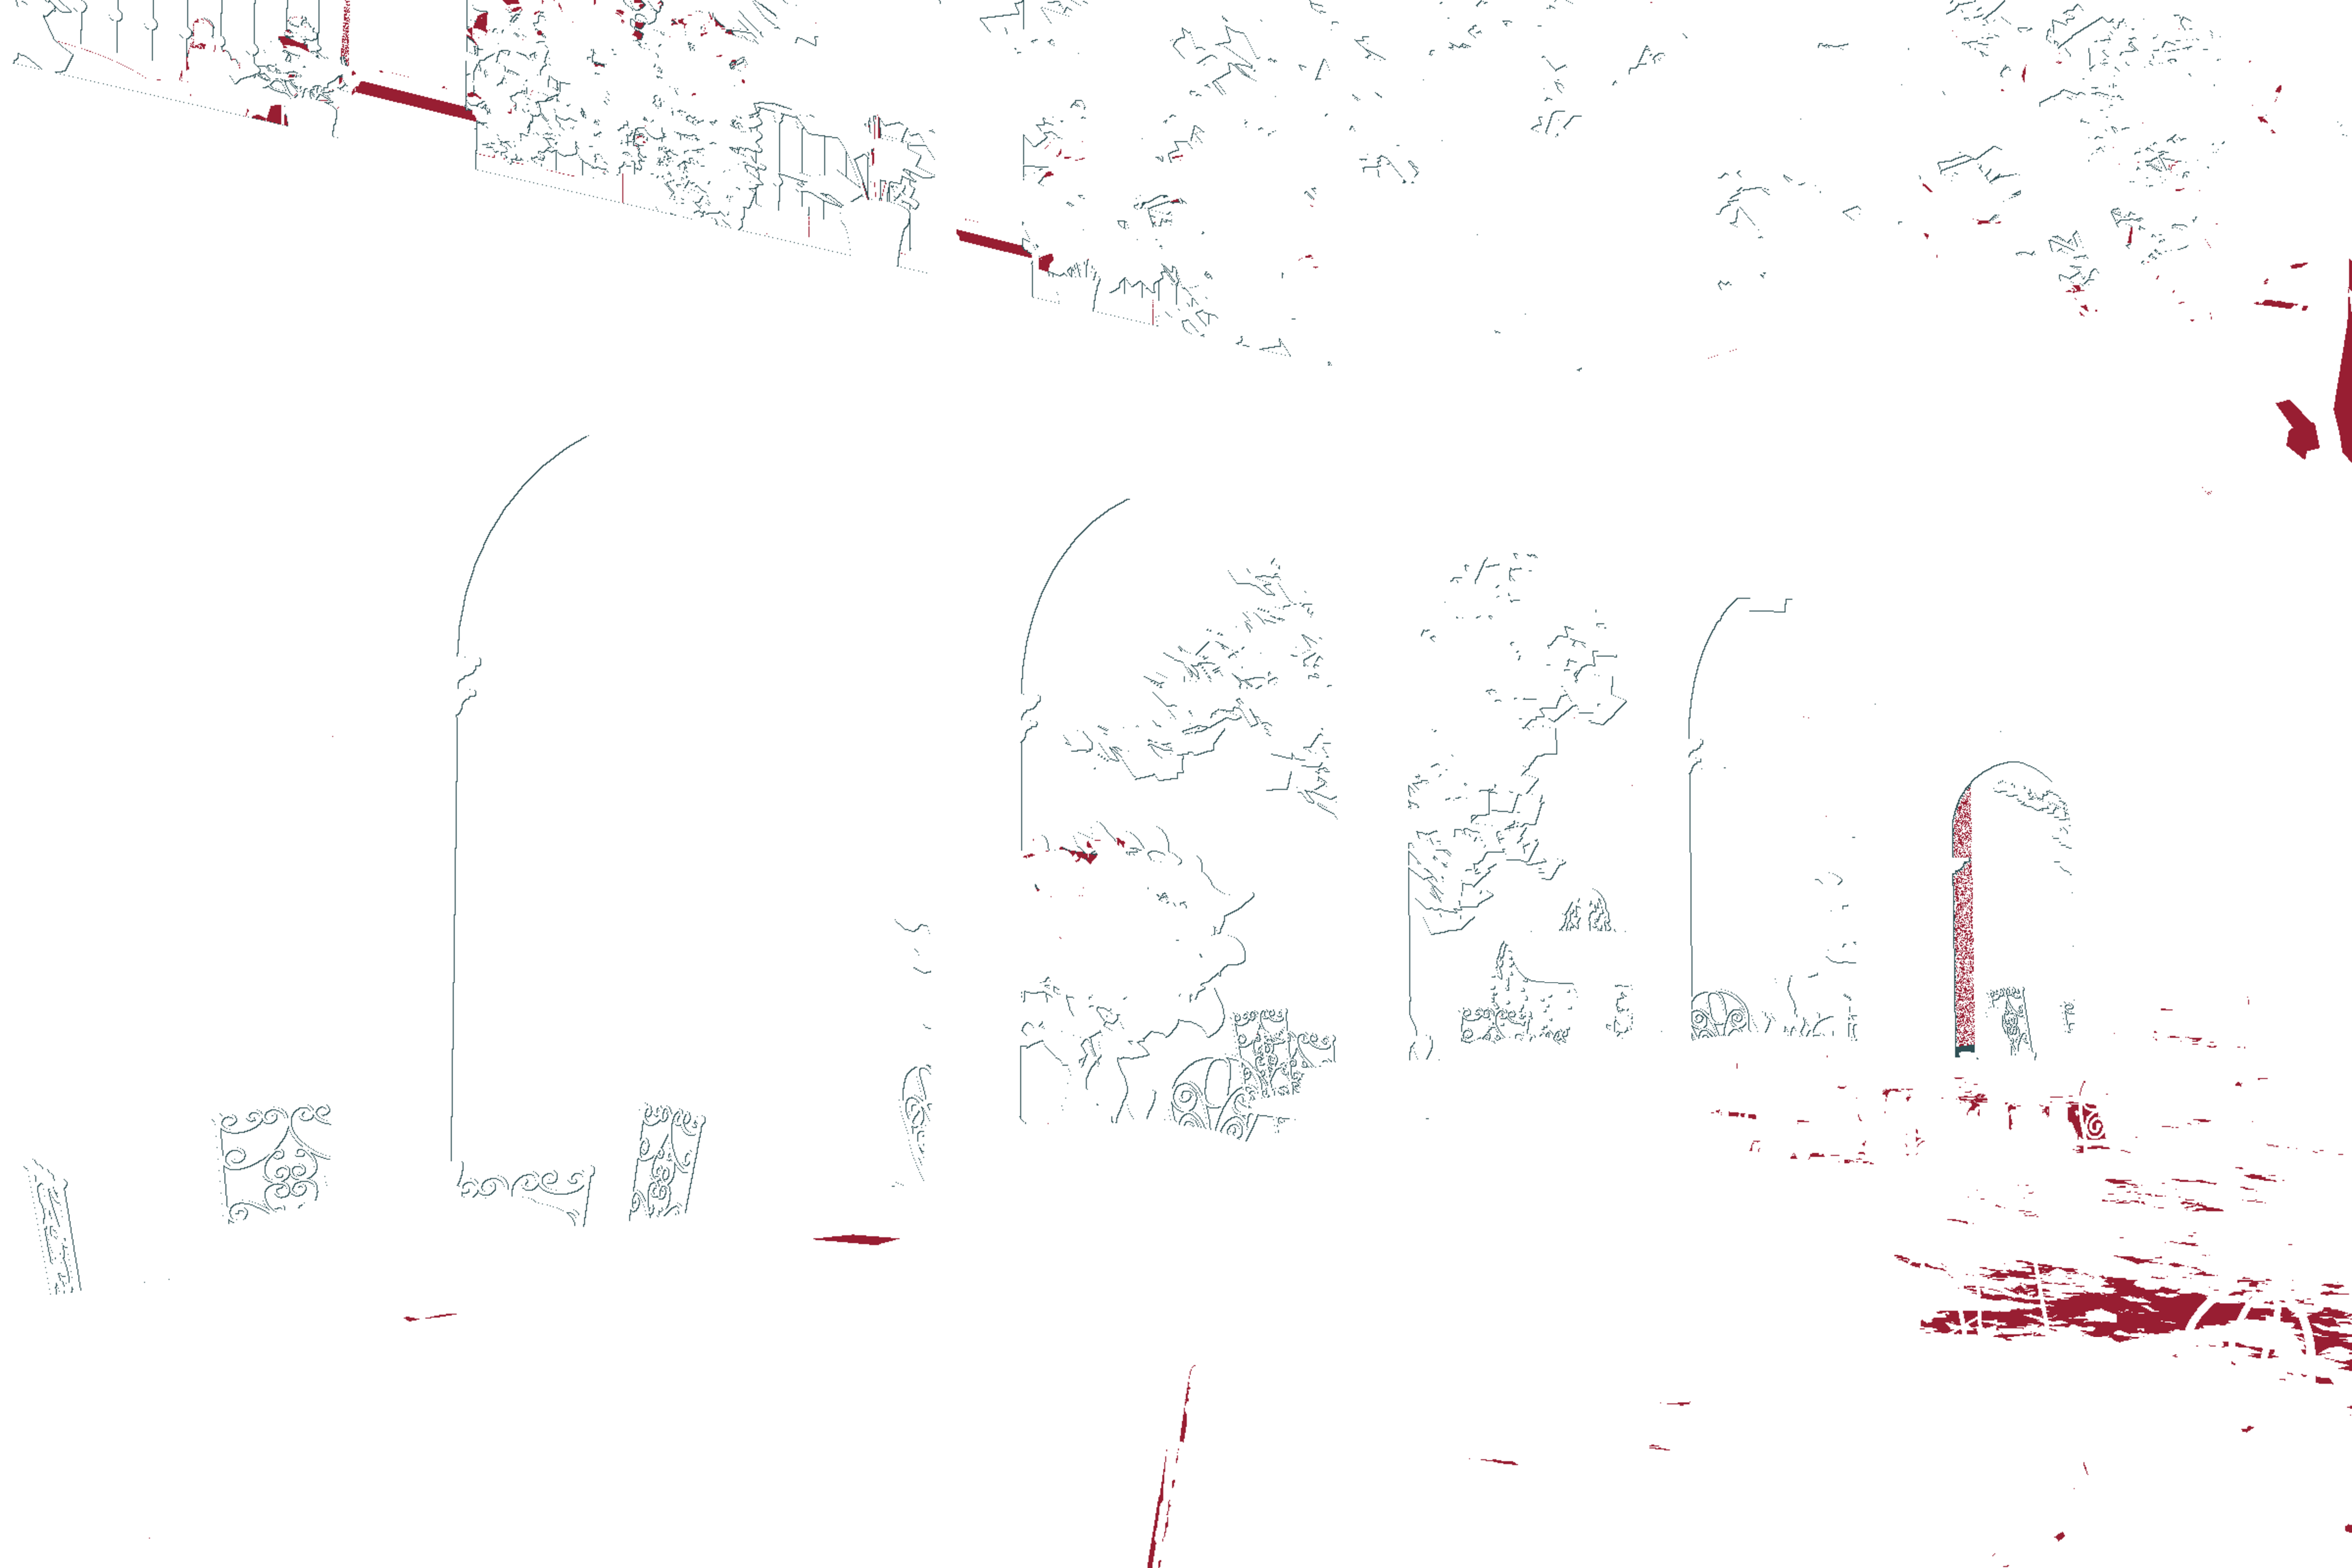
\includegraphics[width=6in]{drawings/test_case/results/analysis/shadow_0_diff.pdf}%
} \\
\end{tabular}}
\caption{8-Voxel Test Case - Composited Image using no Shadow
Mesh}
\label{fig:san-miguel-8-composite-0}
\end{figure}

\begin{figure}
\setlength\tabcolsep{0pt}
\noindent\makebox[\textwidth]{%
\begin{tabular}{ c }
\fcolorbox{wsu-gray}{white}{%
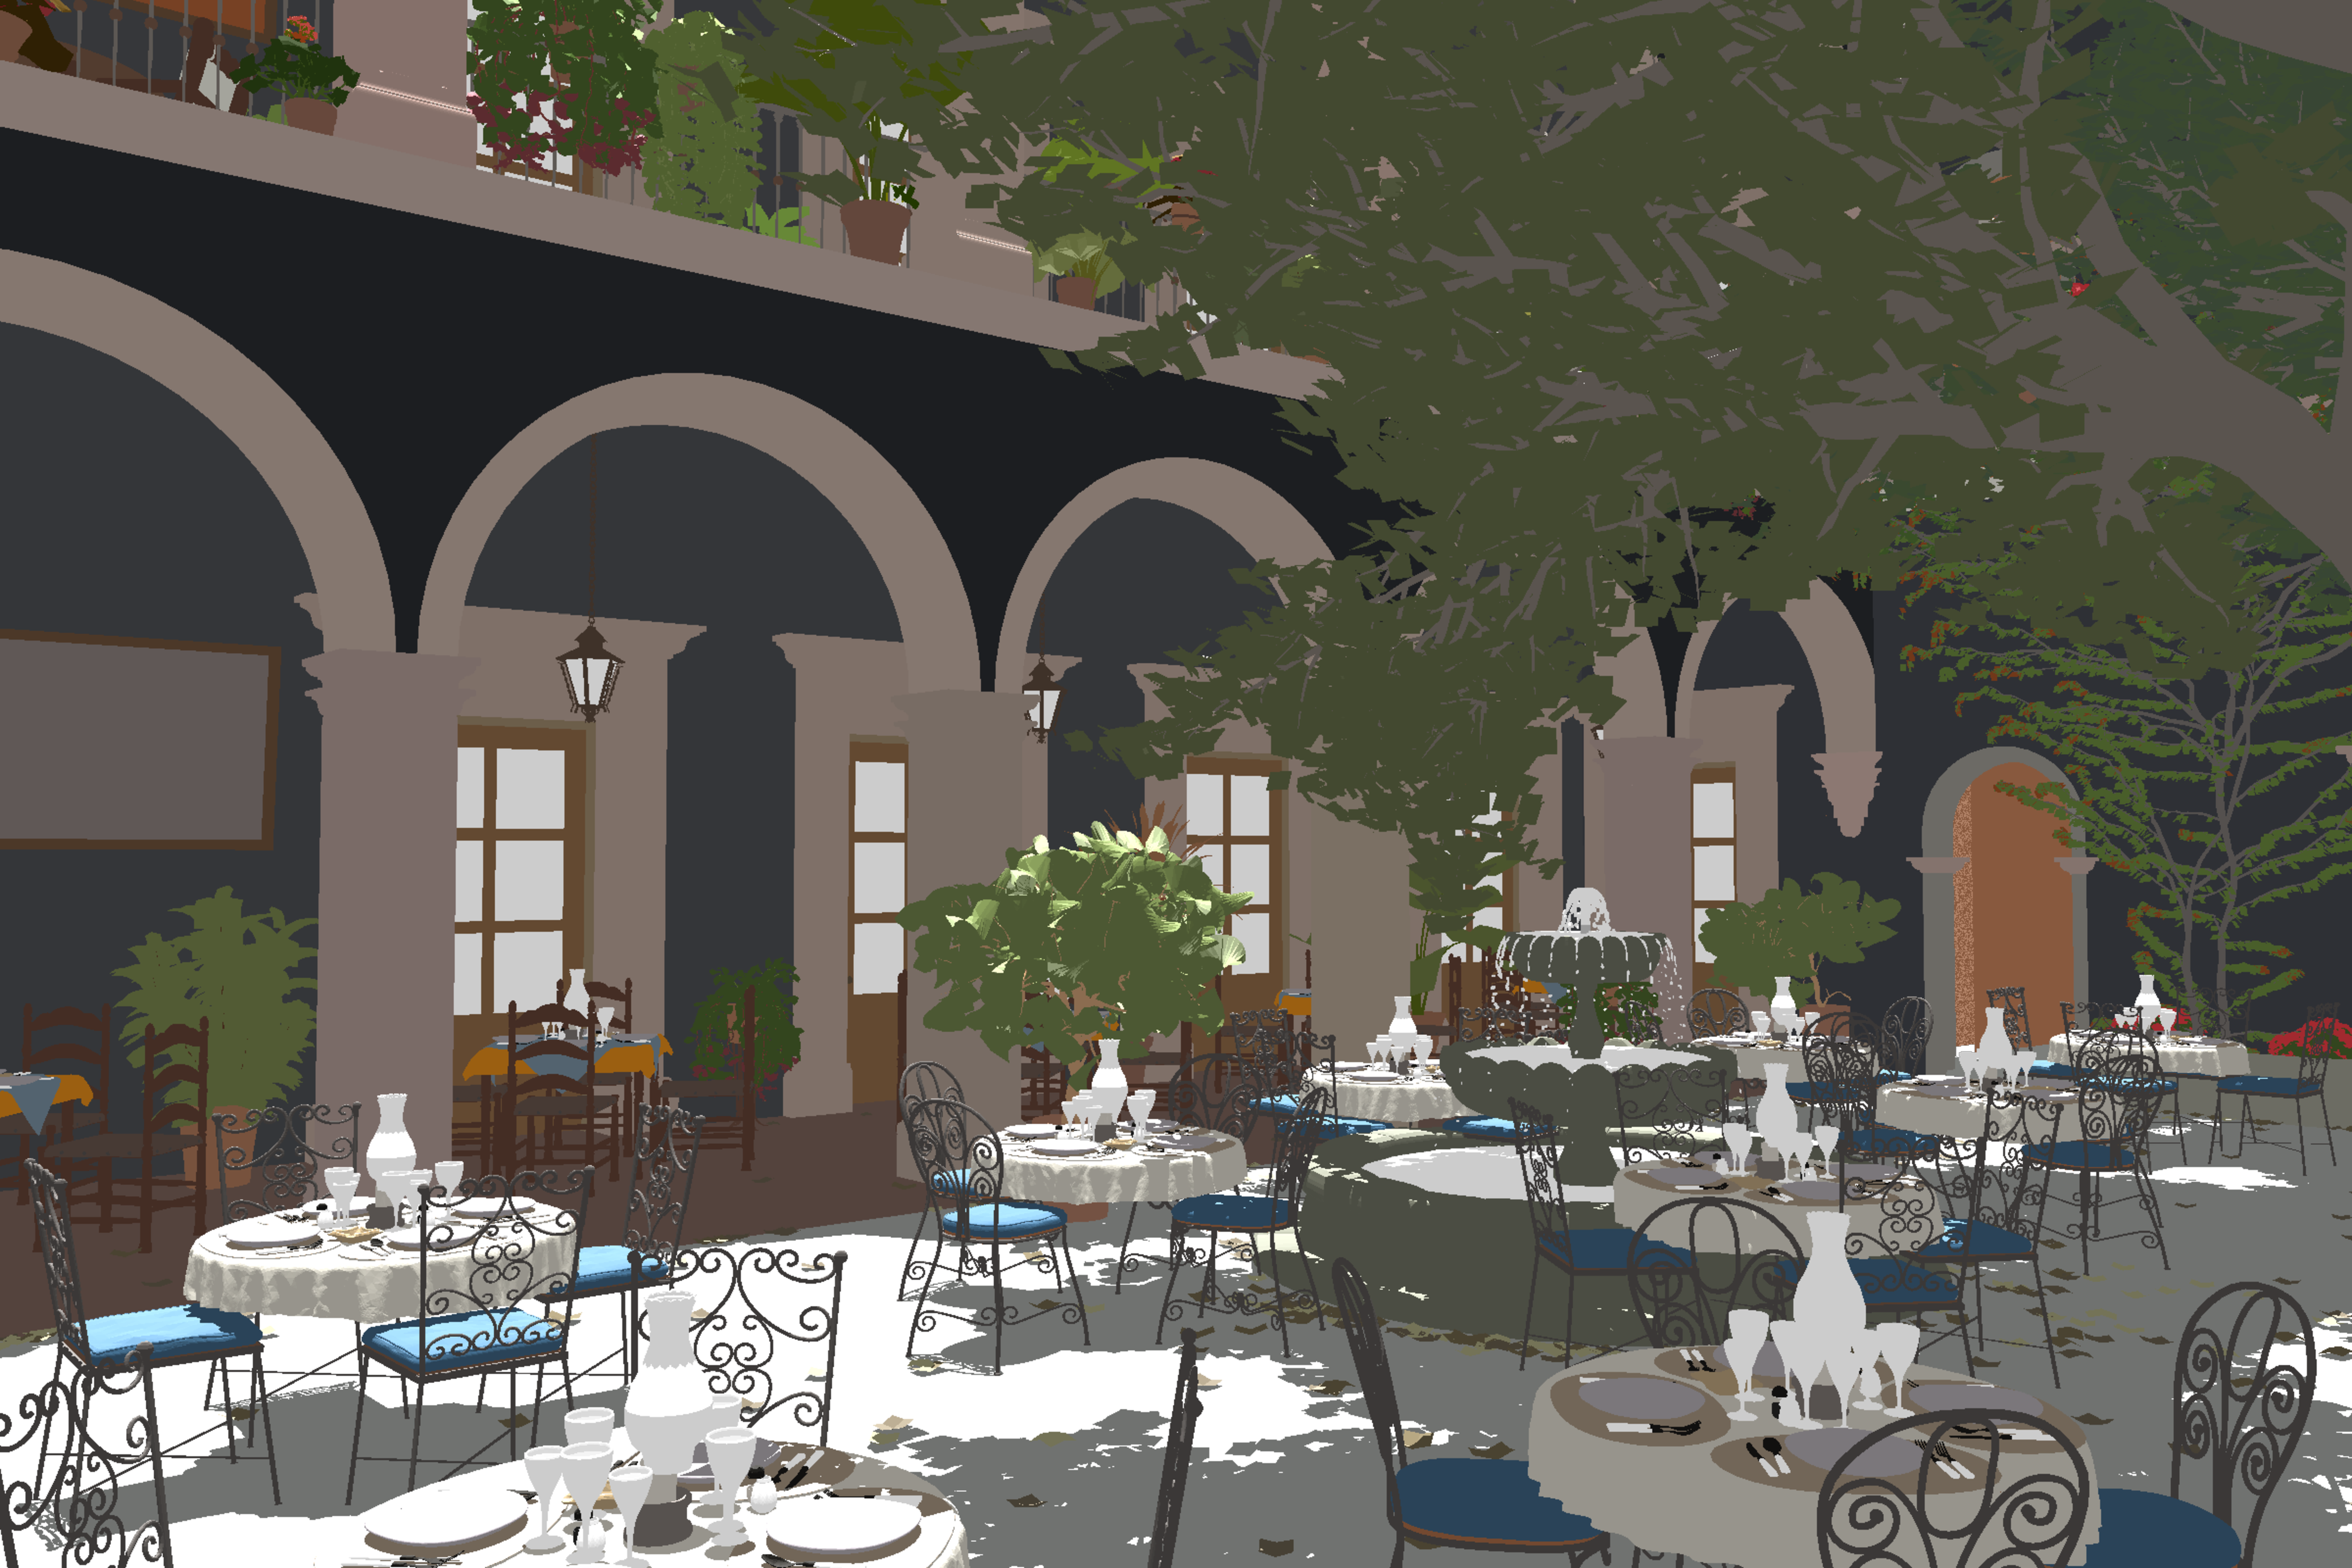
\includegraphics[width=6in]{drawings/test_case/results/analysis/image_8_shadow_100.pdf}%
} \\
\fcolorbox{wsu-gray}{white}{%
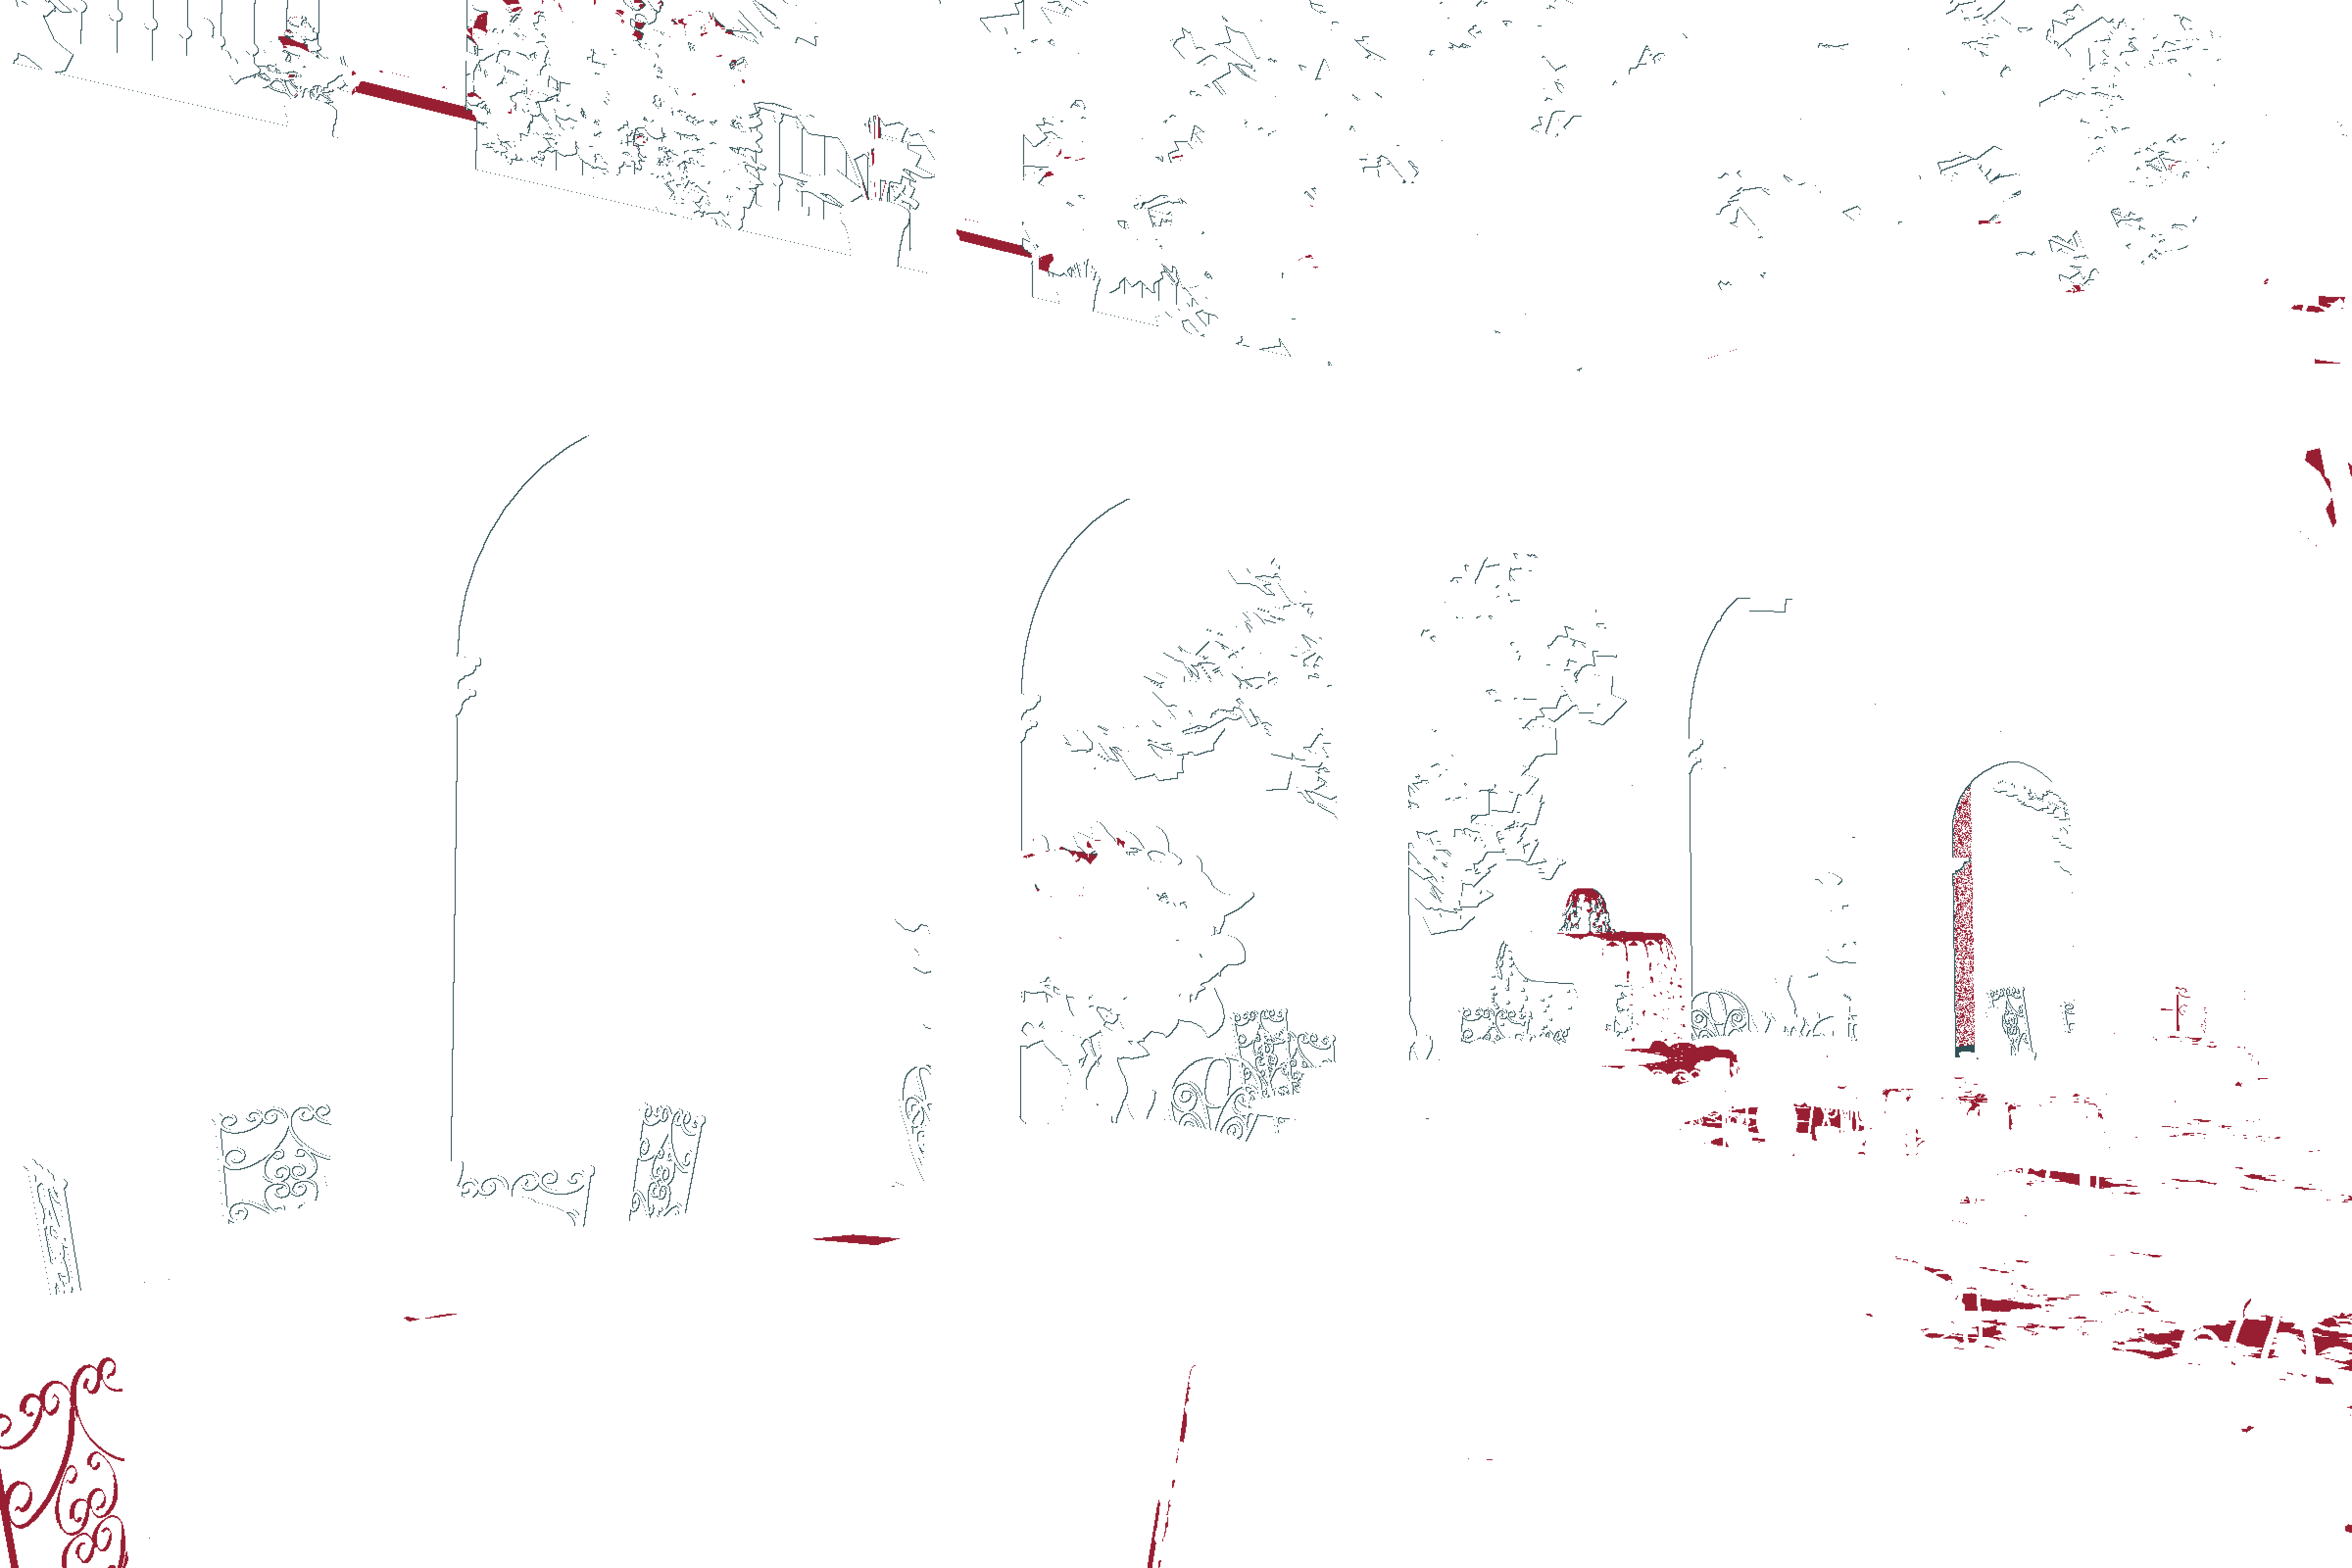
\includegraphics[width=6in]{drawings/test_case/results/analysis/shadow_100_diff.pdf}%
} \\
\end{tabular}}
\caption{8-Voxel Test Case - Composited Image using 100$^2$ Shadow
Mesh}
\label{fig:san-miguel-8-composite-100}
\end{figure}

\begin{figure}
\setlength\tabcolsep{0pt}
\noindent\makebox[\textwidth]{%
\begin{tabular}{ c }
\fcolorbox{wsu-gray}{white}{%
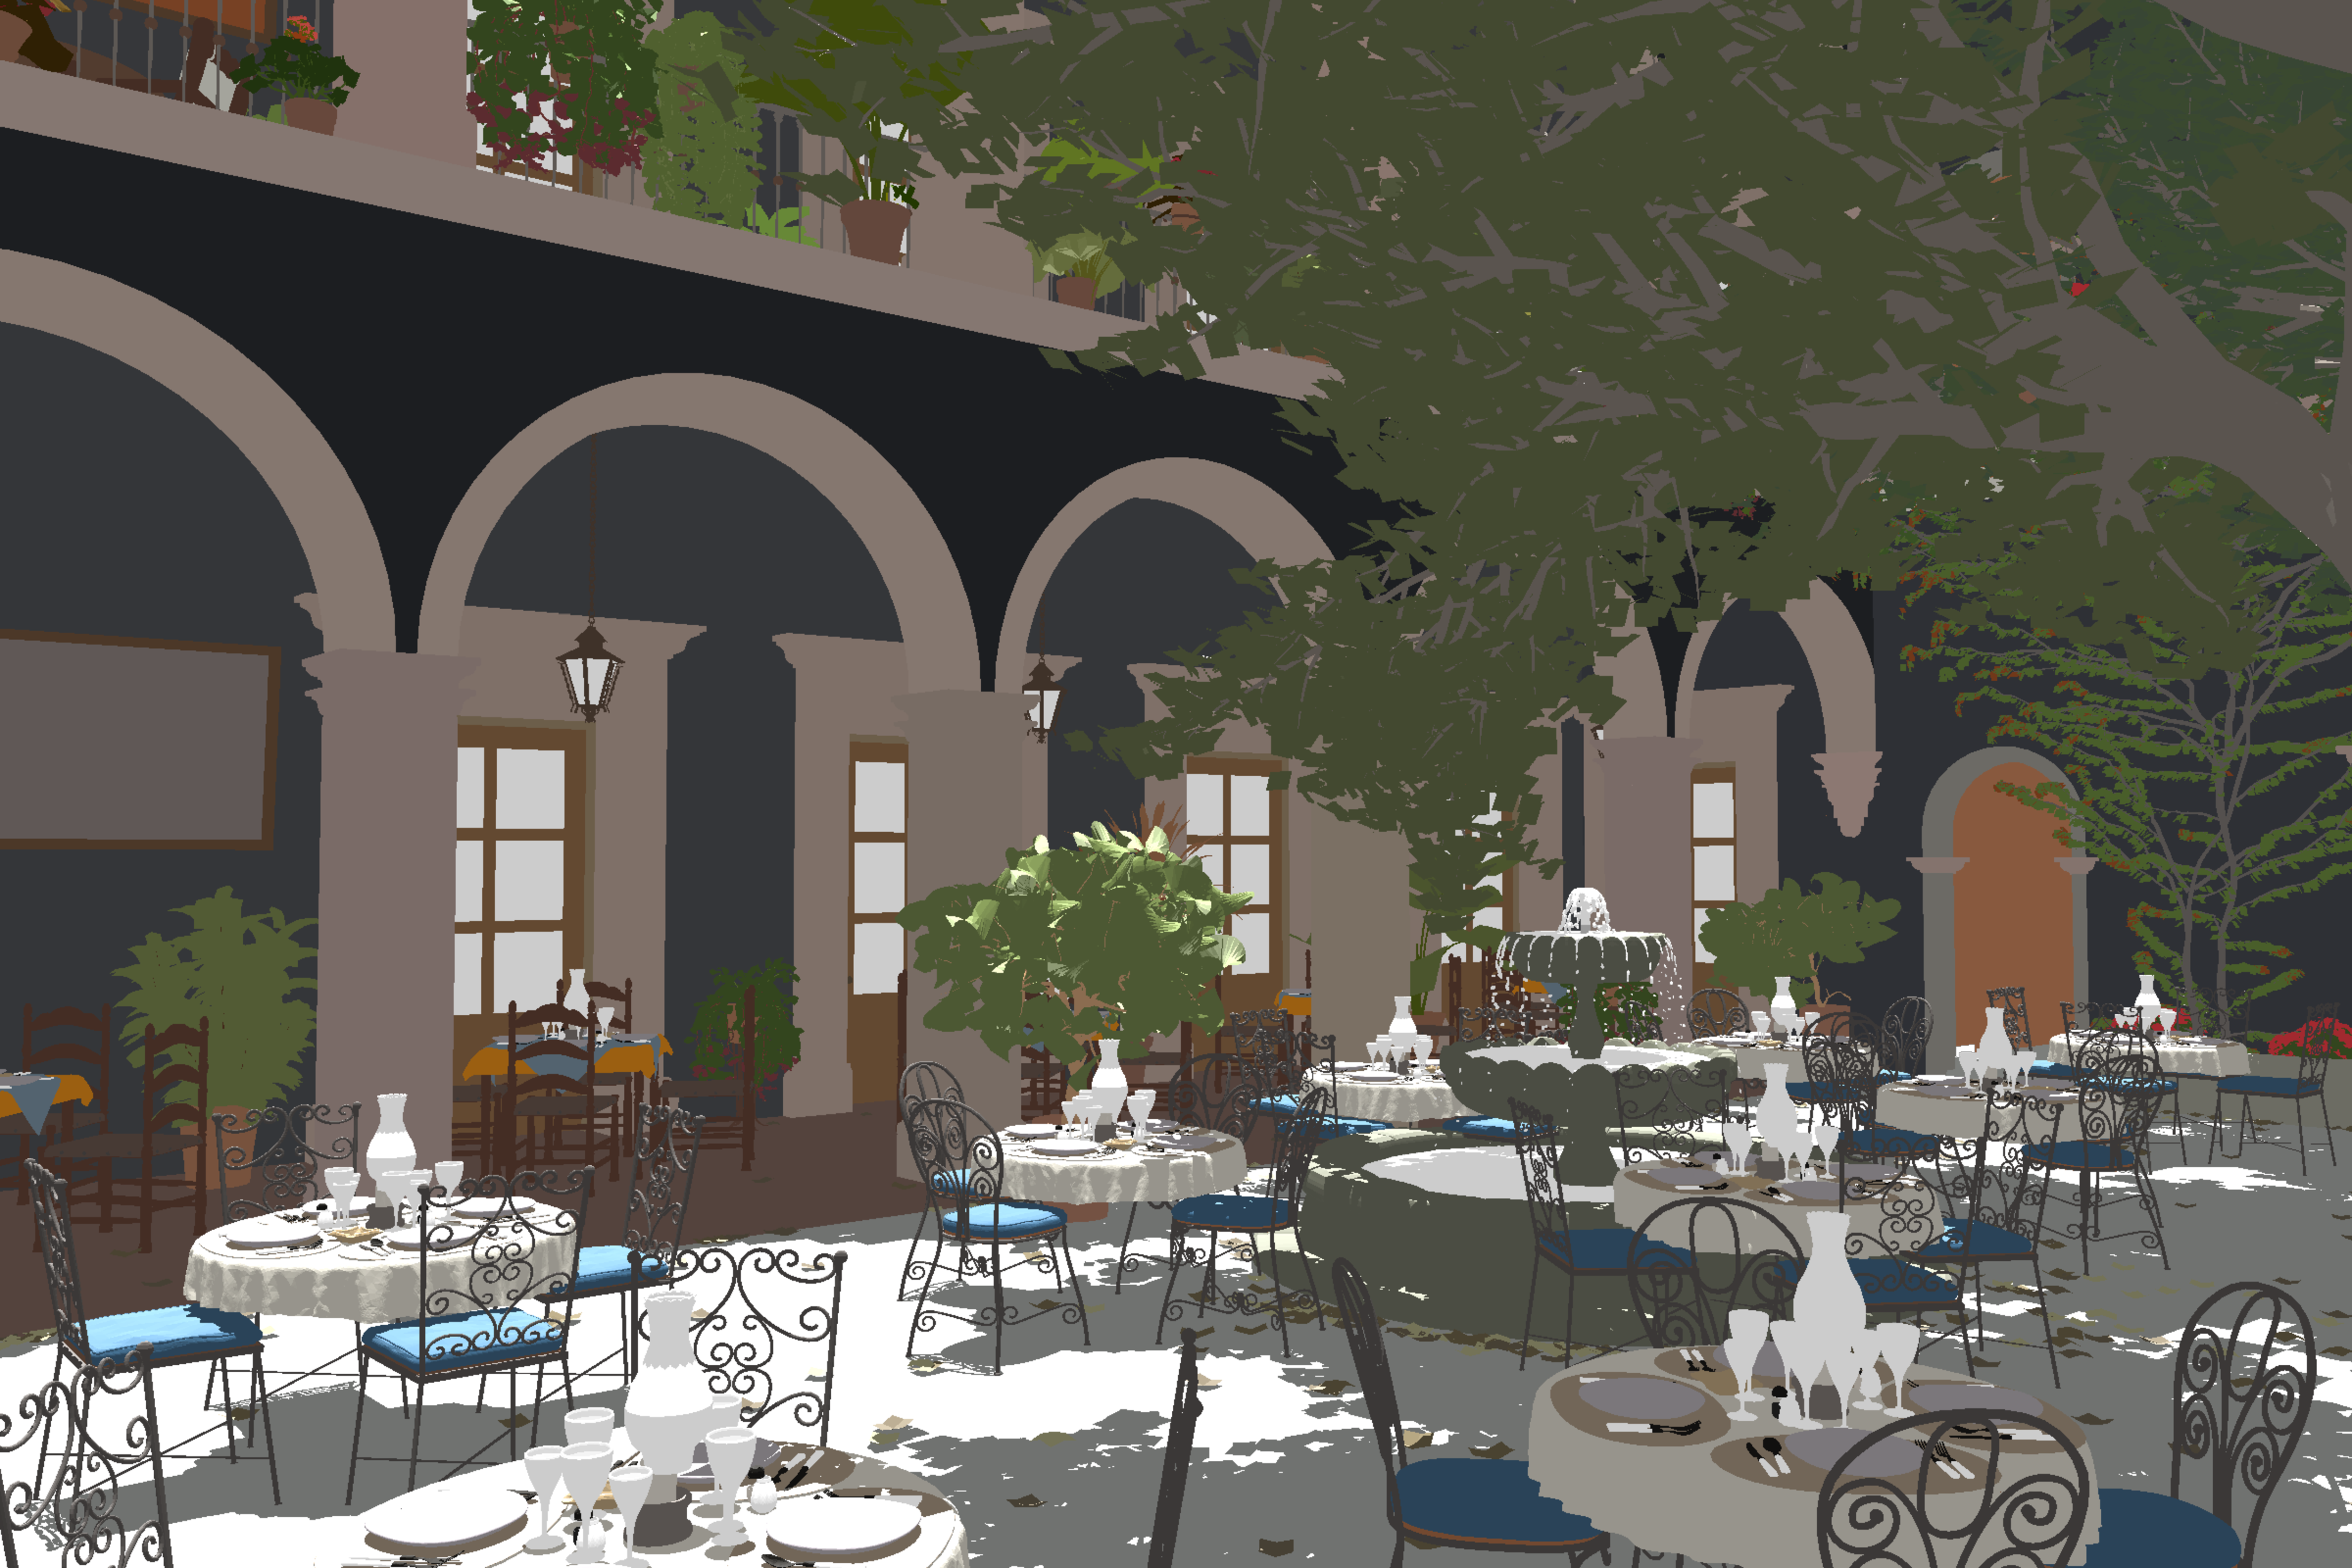
\includegraphics[width=6in]{drawings/test_case/results/analysis/image_8_shadow_1000.pdf}%
} \\
\fcolorbox{wsu-gray}{white}{%
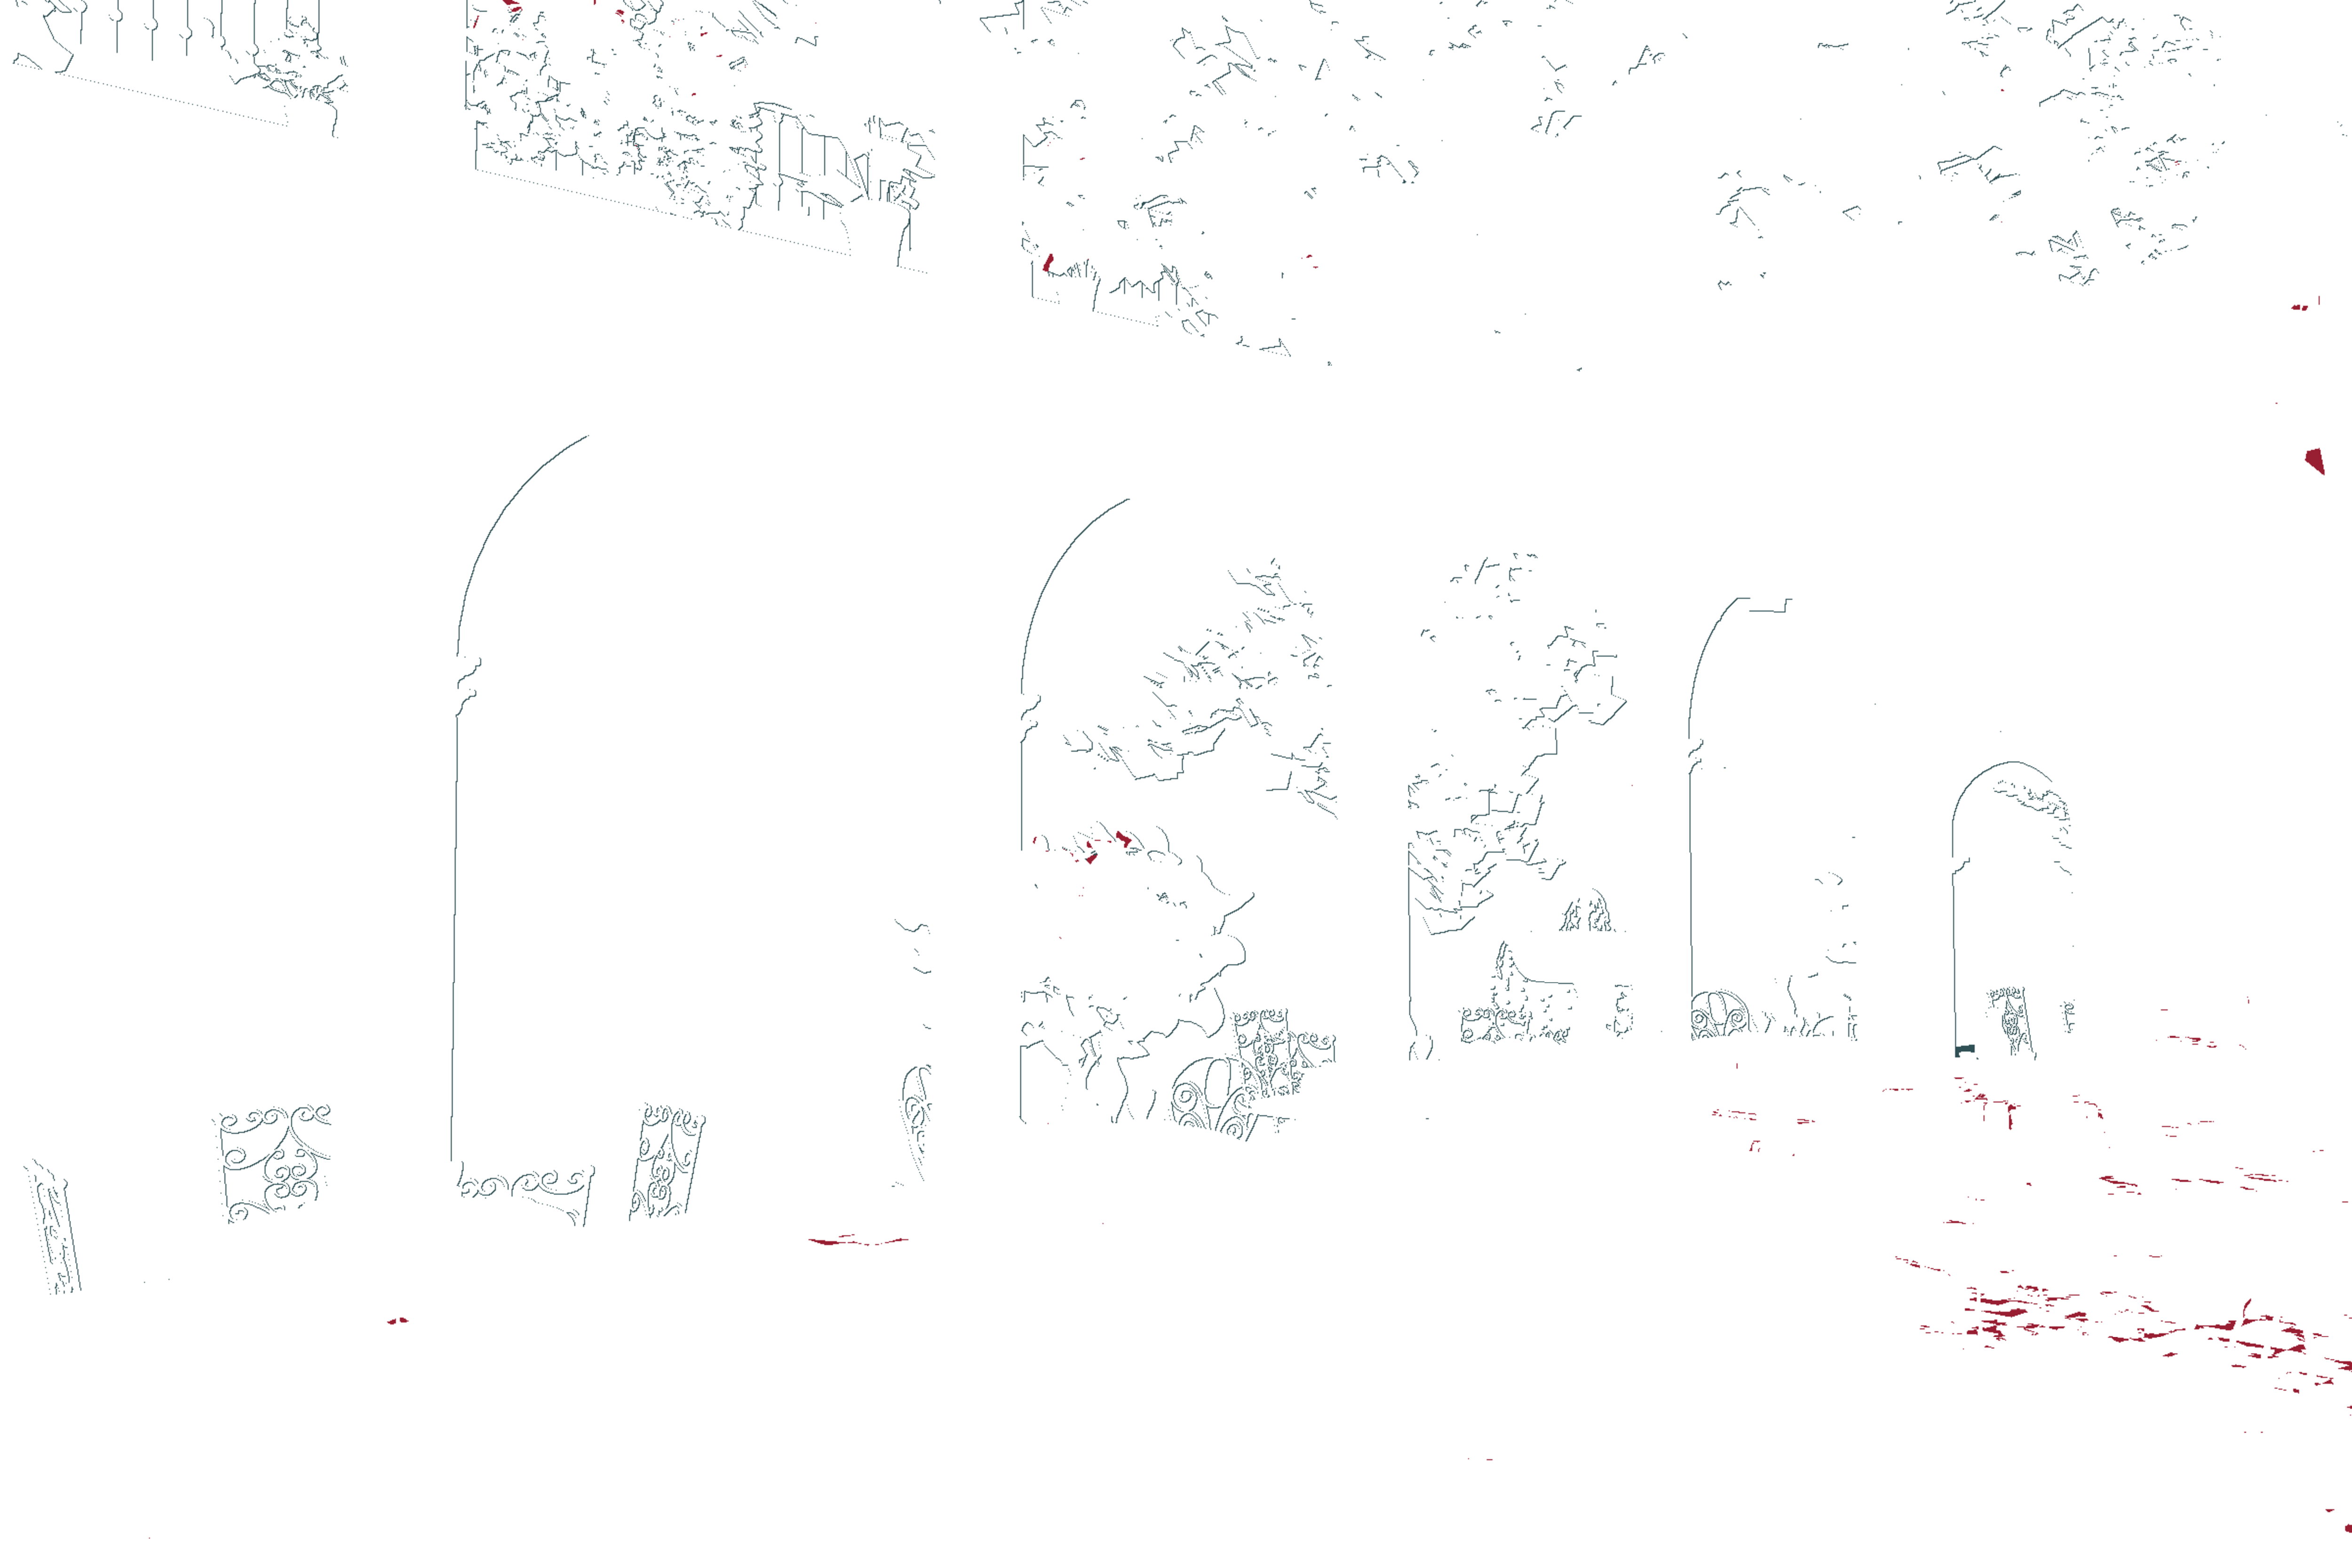
\includegraphics[width=6in]{drawings/test_case/results/analysis/shadow_1000_diff.pdf}%
} \\
\end{tabular}}
\caption{8-Voxel Test Case - Composited Image using 1000$^2$ Shadow
Mesh}
\label{fig:san-miguel-8-composite-1000}
\end{figure}

\begin{figure}
\setlength\tabcolsep{0pt}
\noindent\makebox[\textwidth]{%
\begin{tabular}{ c }
\fcolorbox{wsu-gray}{white}{%
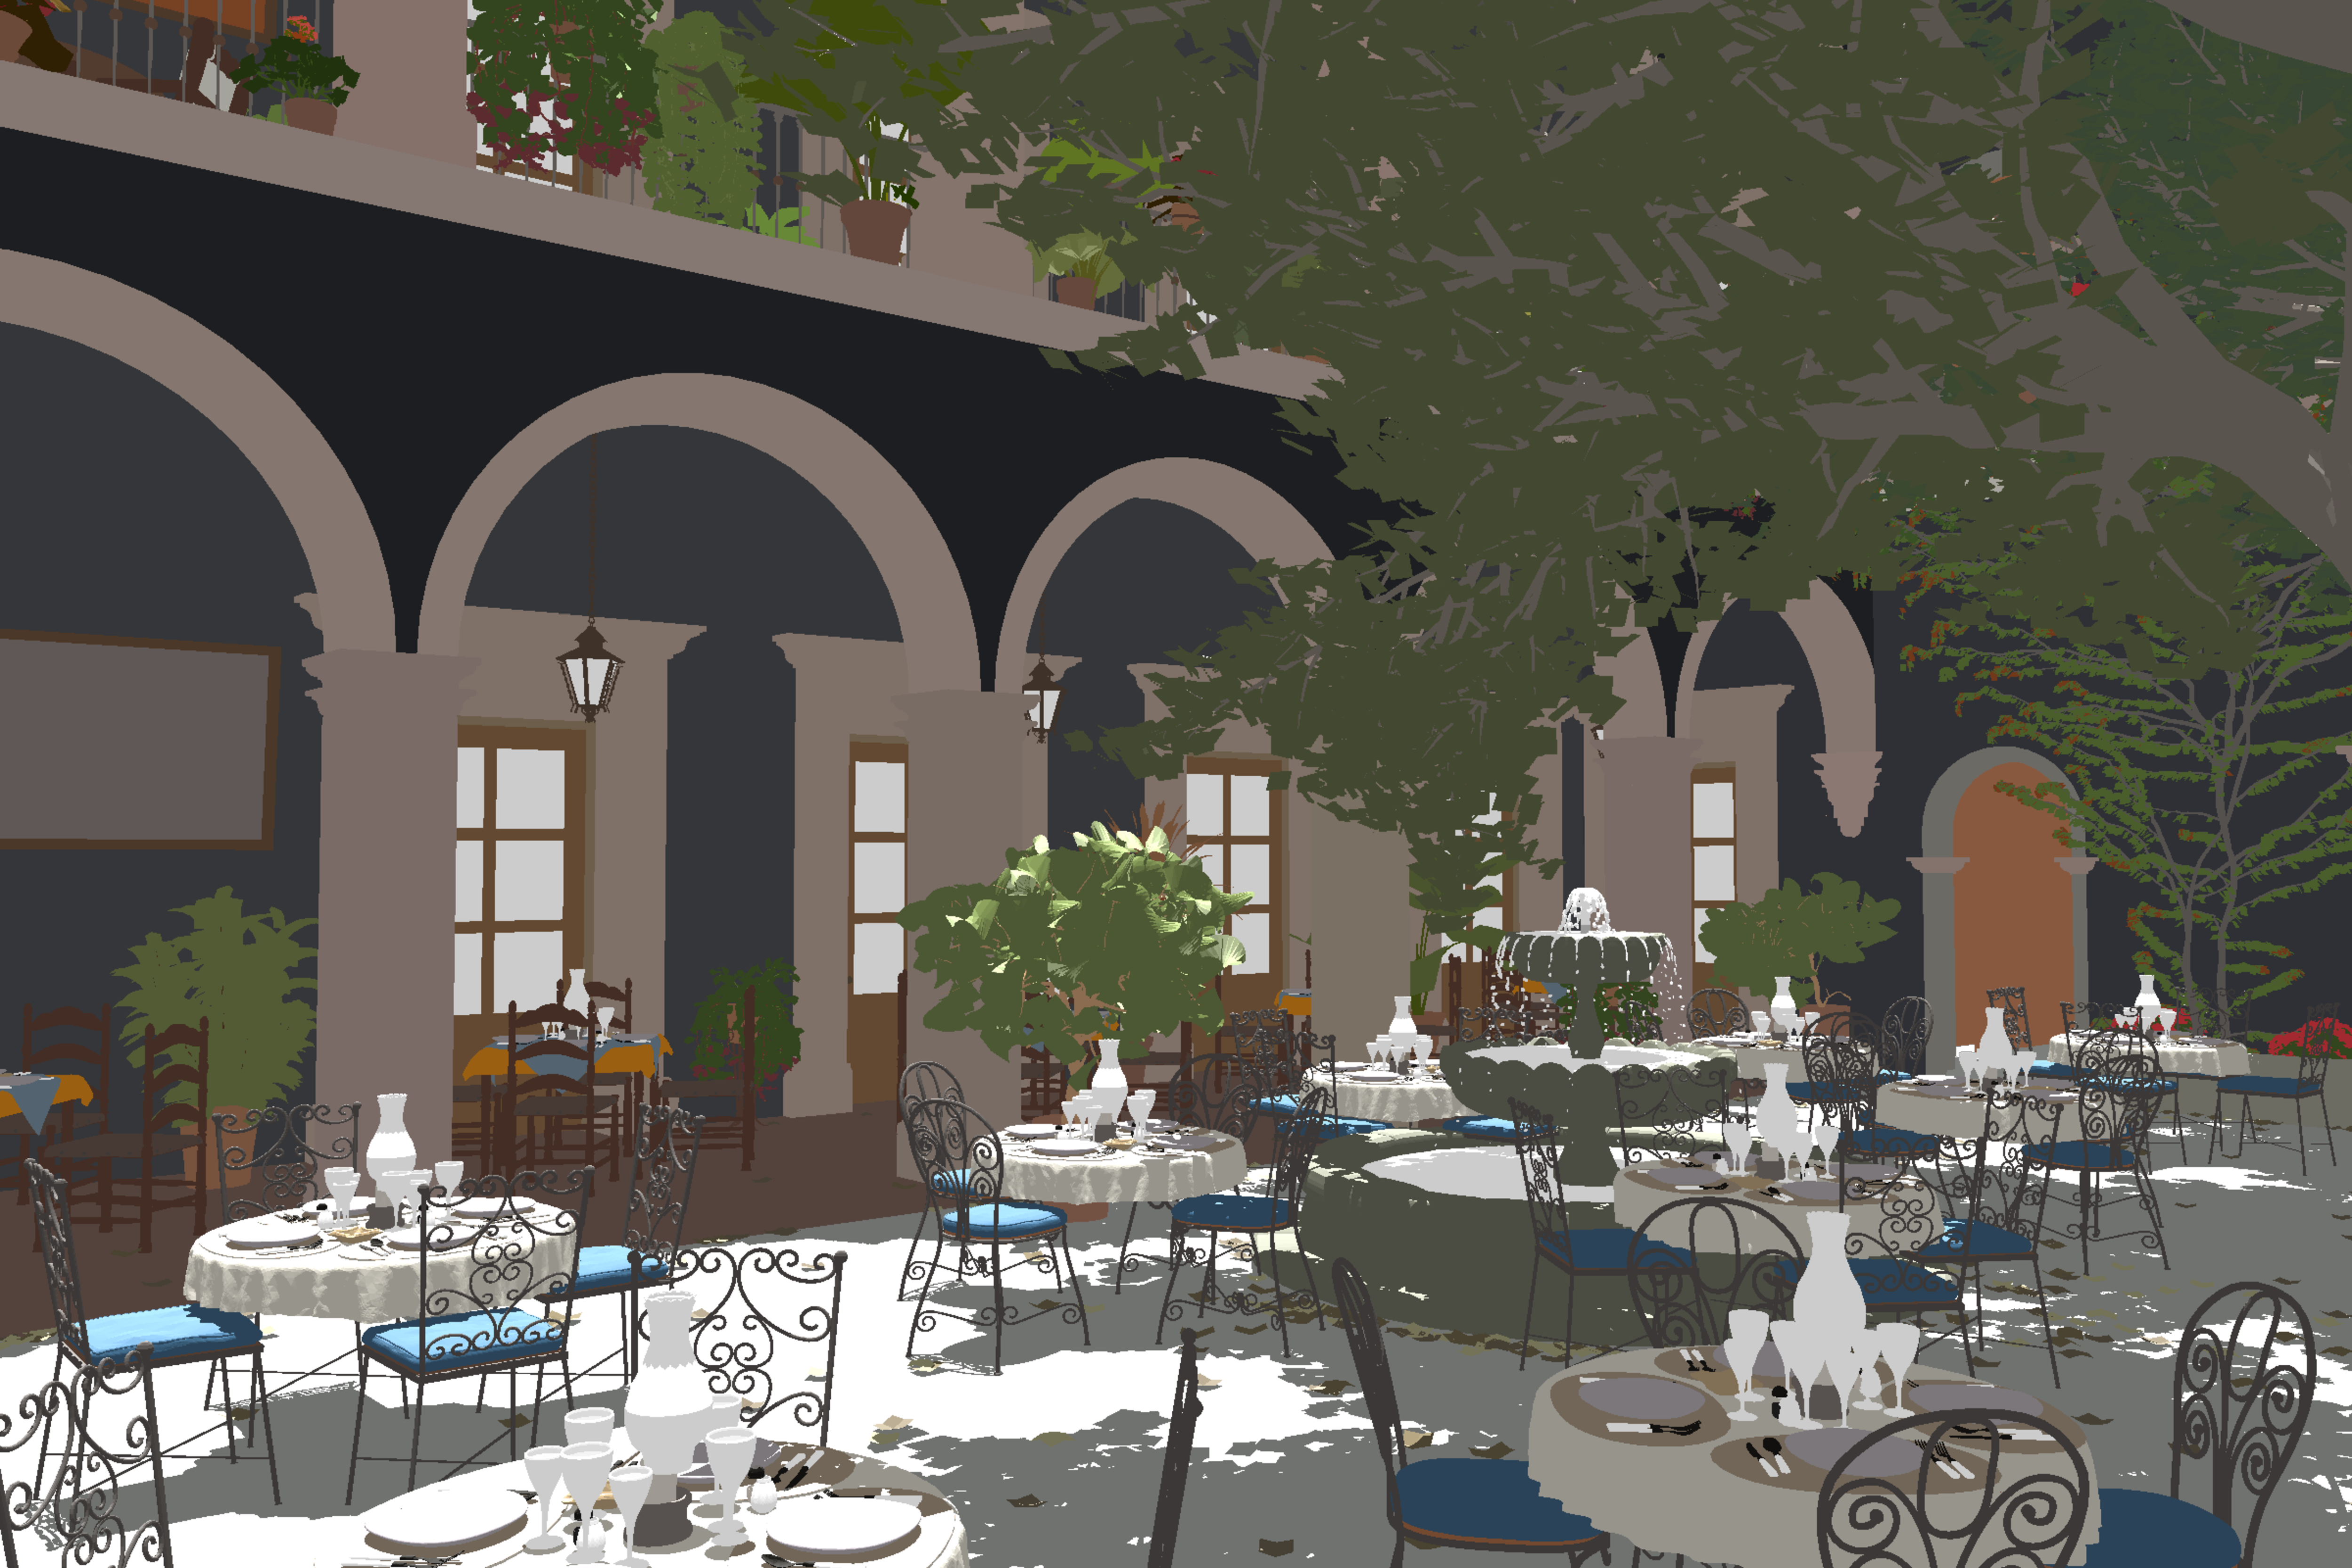
\includegraphics[width=6in]{drawings/test_case/results/analysis/image_8_shadow_10000.pdf}%
} \\
\fcolorbox{wsu-gray}{white}{%
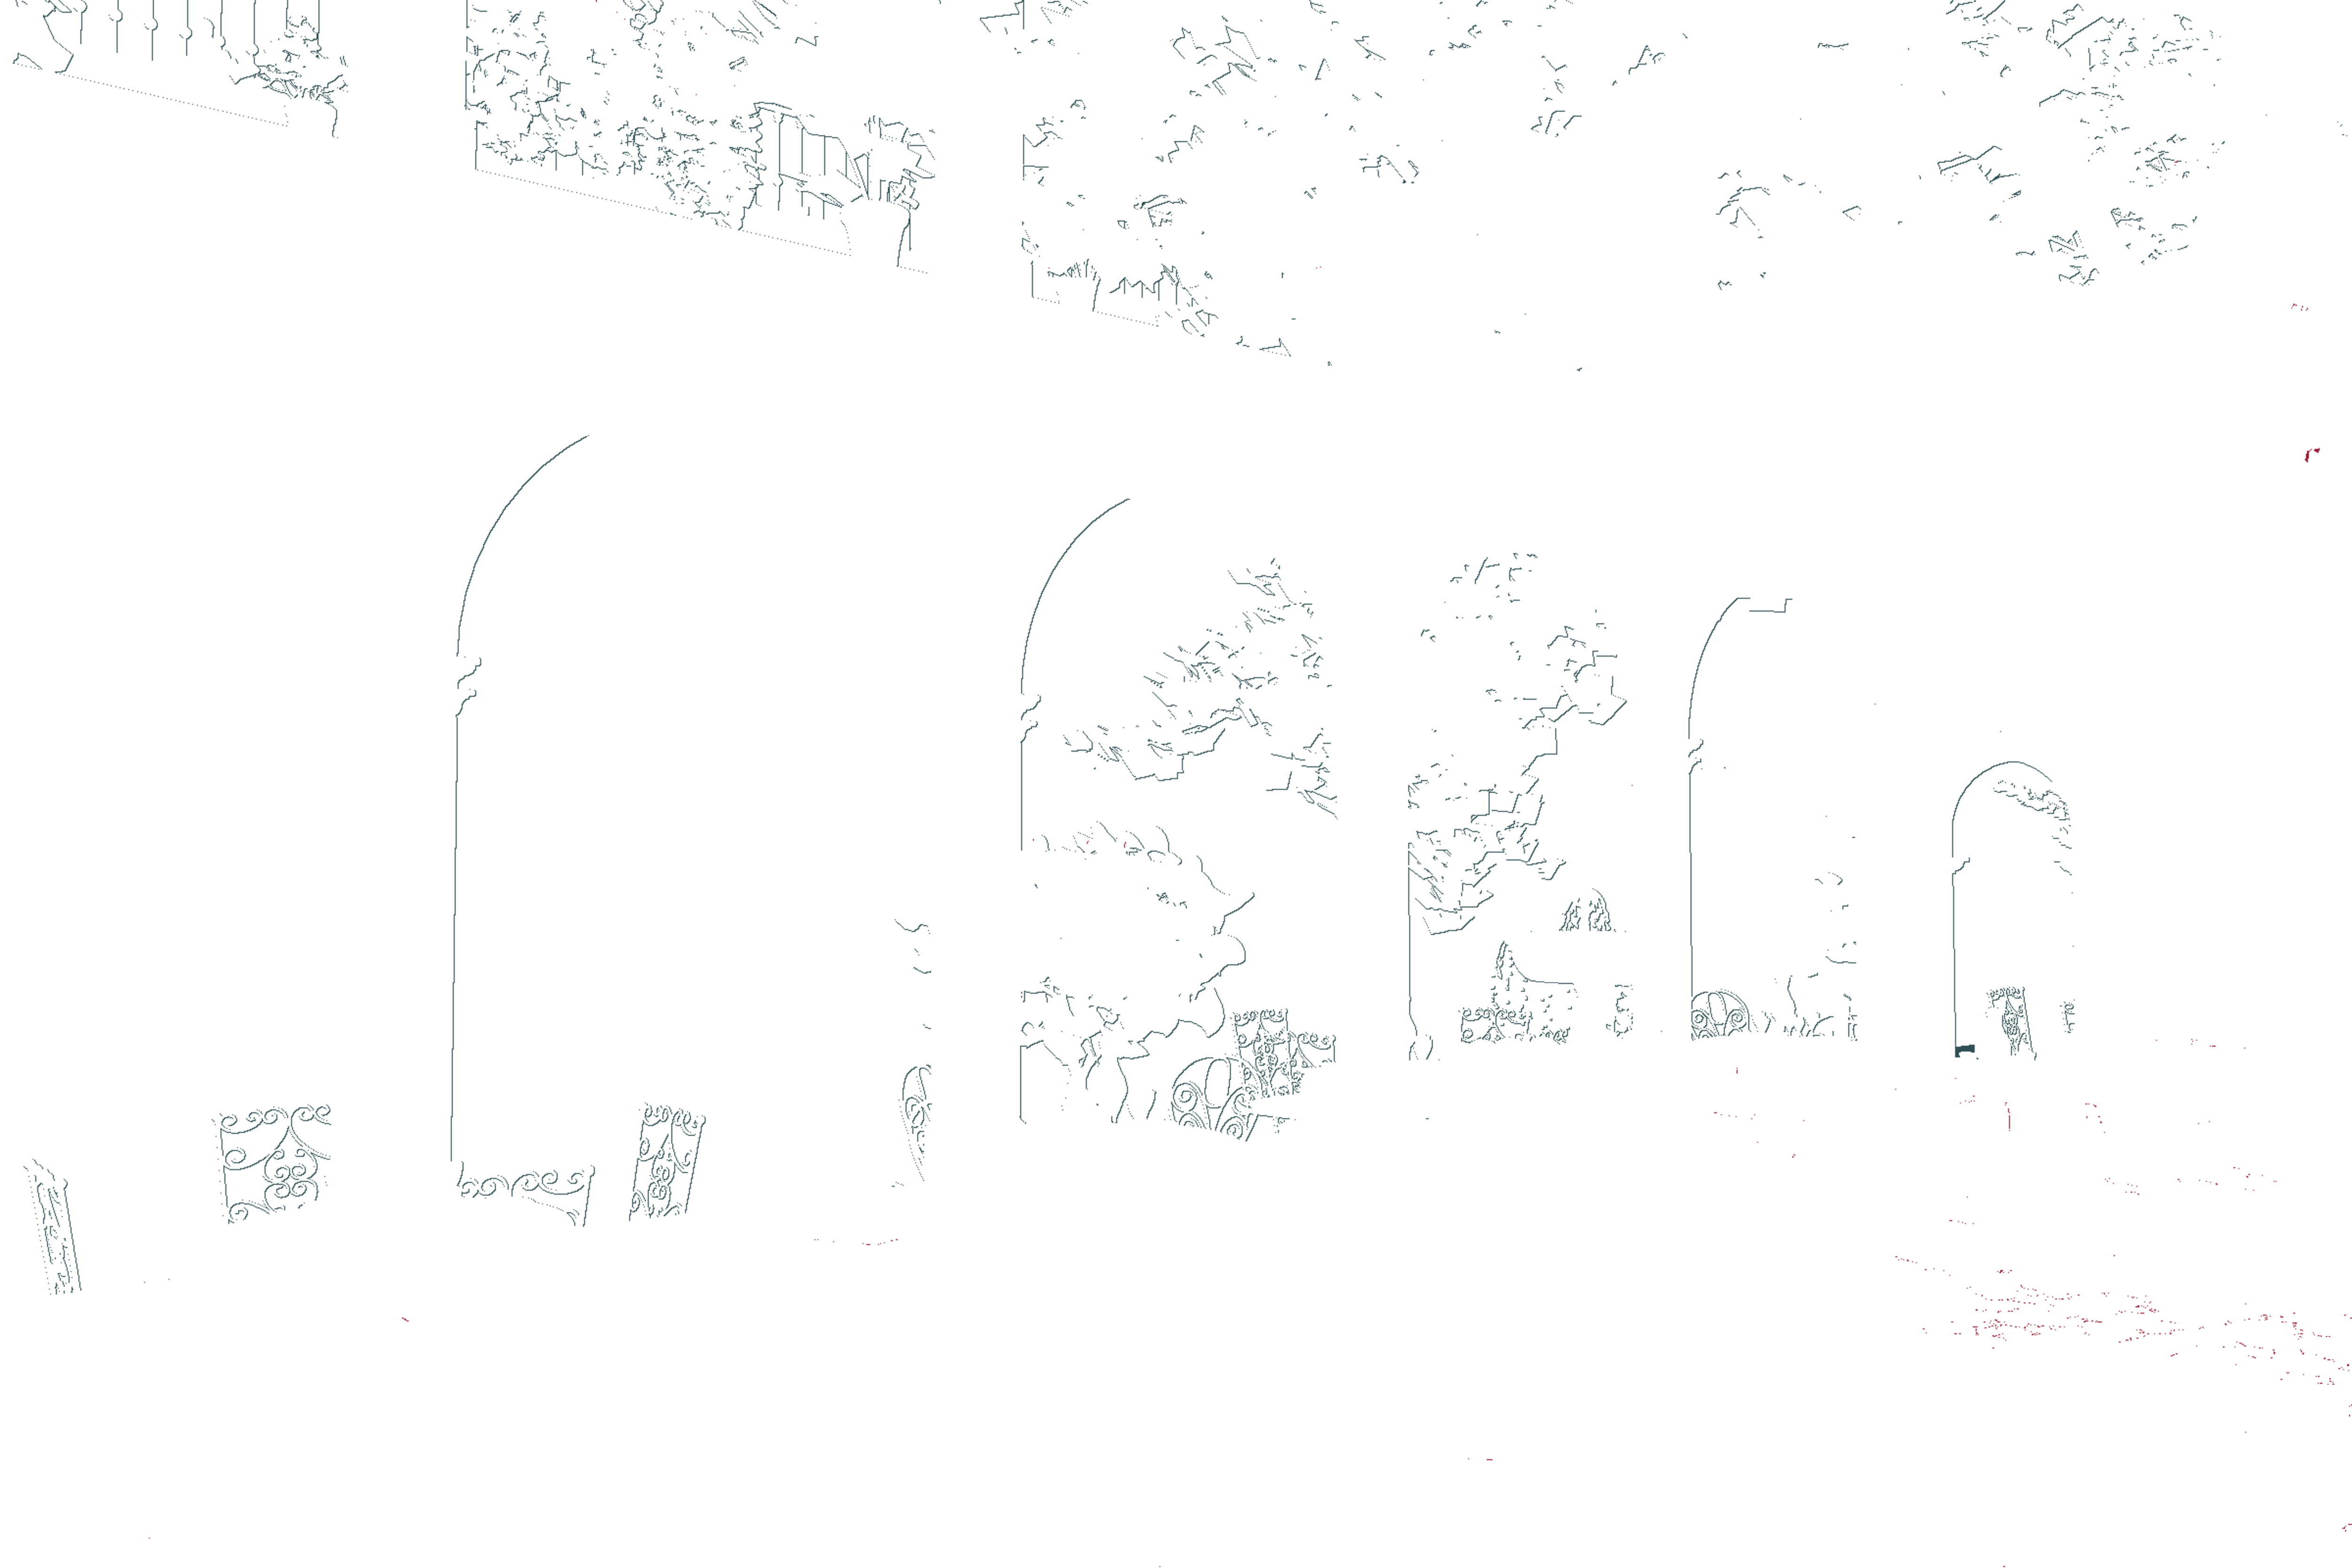
\includegraphics[width=6in]{drawings/test_case/results/analysis/shadow_10000_diff.pdf}%
} \\
\end{tabular}}
\caption{8-Voxel Test Case - Composited Image using 10000$^2$ Shadow
Mesh}
\label{fig:san-miguel-8-composite-10000}
\end{figure}

\newpage
\section{Performance}
\label{sec:performance}
Table~\ref{tbl:performance-load} shows the average time to complete loading the
San Miguel scene into memory for the indicated number of nodes.  The max time to
load a single voxel from each set of voxel decompositions is included in the last
column.  For our test cases, splitting the scene into voxels was done as a
pre-processing step.  We can see from the results that the time to load the
scene in partial pieces is roughly equivalent to the time required to load the entire
scene.  As we add nodes, we see a decline in the total time needed to load the
scene for larger voxel counts as the work is split across the nodes.  The worst
case time to load all voxels on all nodes will be at least as good as the times
indicated in the \emph{max} column. \\

\begin{table}[!htb]
\centering
\begin{tabular}{ | c | r | m{0.8in} m{0.8in} m{0.8in} m{0.8in} m{0.8in} | }
\hline
\multicolumn{2}{| l }{Nodes} & 1 & 2 & 4 & 8 & Max  
\\
\hline
\multirow{4}{*}{\rotatebox[origin=c]{90}{Voxels}}
& 1   & 60.3 (0.7)  & - & - & - & 60.3 (0.7) \\
& 8   & 59.3 (0.4)  & 29.7          & 14.8    & 7.4     & 38.9 (0.2) \\
& 27  & 58.0 (0.4)  & 29.0          & 14.5    & 7.2     & 24.6 (0.2) \\
& 64  & 58.9 (0.4)  & 29.4          & 14.7    & 7.4     & 24.6 (0.1) \\
\hline
\end{tabular}
\caption{Execution Time (Seconds) - Load Voxels}
\label{tbl:performance-load}
\end{table}

Table~\ref{tbl:compute-shadow-mesh} shows the average time to compute and trace
the viewing rays to produce shadows meshes with the resolution indicated.
As the size of the mesh increases, the time to compute the mesh increases.

\begin{table}[!htb]
\centering
\begin{tabular}{ | l | c | c | r | m{0.8in} m{0.8in} m{0.8in} m{0.8in} m{0.8in}
| }
\hline
\multicolumn{4}{| l }{Nodes} & 1 & 2 & 4 & 8 & Max \\
\hline
\multirow{12}{*}{\rotatebox[origin=c]{90}{Resolution}}
& \multirow{4}{*}{\rotatebox[origin=c]{90}{100$^{2}$}}
& \multirow{12}{*}{\rotatebox[origin=c]{90}{Voxels}}
& 1  & 1.3 (0.2) ms & - & - & - & - \\
& & & 8  & 0.7 (0.1) ms & 0.3 ms & 0.2 ms & 0.1 ms & 0.8 (0.5) ms \\
& & & 27 & 0.7 (0.1) ms & 0.3 ms & 0.2 ms & 0.1 ms & 1.2 (0.5) ms \\
& & & 64 & 0.6 (0.2) ms & 0.3 ms & 0.2 ms & 0.1 ms & 1.5 (0.7) ms \\
\cline{4-9}
\cline{2-2}
& \multirow{4}{*}{\rotatebox[origin=c]{90}{1000$^{2}$}}
& & 1   & 86 (2) ms & - & - & - & - \\
& & & 8  & 58 (1) ms & 29 ms & 14 ms & 7 s & 60 (1) ms \\
& & & 27 & 49 (3) ms & 24 ms & 12 ms & 6 s & 84 (2) ms \\
& & & 64 & 45 (2) ms & 22 ms & 11 ms & 6 s & 118 (1) ms \\
\cline{4-9}
\cline{2-2}
& \multirow{4}{*}{\rotatebox[origin=c]{90}{10000$^{2}$}}
& & 1  & 8.1 (0.1) s & - & - & - & - \\
& & & 8  & 5.7 (0.1) s & 2.8 s & 1.4 s & 0.7 s & 5.9 (0.2) s \\
& & & 27 & 4.8 (0.2) s & 2.4 s & 1.2 s & 0.6 s & 8.3 (0.1) s \\
& & & 64 & 4.3 (0.1) s & 2.2 s & 1.1 s & 0.5 s & 11.7 (0.3) s \\
\hline
\end{tabular}
\caption{Execution Time - Trace Light Rays}
\label{tbl:compute-shadow-mesh}
\end{table}

Table~\ref{tbl:performance-trace} shows the average time to trace all voxels.
The max time to trace a single voxel from each set of voxel decompositions is
given in the last column.  As we increase the number of voxels, the time on a
single node to trace the scene increases.  This suggests a upper bound on the
number of voxels a scene should be split into and is correlated with the number
of nodes available.

\begin{table}[!htb]
\centering
\begin{tabular}{ | c | r | m{0.8in} m{0.8in} m{0.8in} m{0.8in} m{0.8in} | }
\hline
\multicolumn{2}{| l }{Nodes} & 1 & 2 & 4 & 8 & Max   \\
\hline
\multirow{4}{*}{\rotatebox[origin=c]{90}{Voxels}}
& 1  & 31.80   & -       & -       & -       & 31.80 \\
& 8  & 41.83   & 20.91   & 10.46   & 5.23    & 21.99 \\
& 27 & 57.99   & 29.00   & 14.50   & 7.25    & 24.61 \\
& 64 & 95.37   & 47.68   & 23.84   & 11.92   & 24.57 \\
\hline
\end{tabular}
\caption{Execution Time (Seconds) - Trace Viewing Rays}
\label{tbl:performance-trace}
\end{table}

Table~\ref{tbl:performance-trace} shows the time necessary to composite the
images.  We see that increasing the size of the shadow mesh has little impact on
the time to composite the final image.

\begin{table}[!htb]
\centering
\begin{tabular}{ | c | r | m{0.8in} m{0.8in} m{0.8in} m{0.8in} | }
\hline
\multicolumn{2}{| l }{Voxels} & 1 & 8 & 27 & 64 \\
\hline
\multirow{4}{*}{\rotatebox[origin=c]{90}{Resolution}}
& None         & 1.6 (0.2) & 4.0 (0.6)  &           &   \\
& 100$^2$    & 1.6 (0.2) & 3.6 (0.1)  &           &   \\
& 1000$^2$   & 1.6 (0.2) & 3.6 (0.1)  &           &   \\
& 10000$^2$  & 1.7 (0.2) & 3.5 (0.2)  &           &   \\
\hline
\end{tabular}
\caption{Execution Time (Seconds) - Composite Image}
\label{tbl:performance-composite}
\end{table}

The total time to trace the baseline San Miguel scene averages \textasciitilde
90 seconds on a single node.  Introducing our technique for distributing the
scene, computing shadow meshes and compositing a final image increases the
average time to render the scene on a single node with a single voxel to
\textasciitilde 120 seconds.  Increasing the voxel count increases this time,
but we see it can be offset by increasing the number of nodes used.  For our
test case, the optimal runtime was produced by splitting the domain into 8
voxels and running on 8 nodes.  The average time to complete rendering was
reduced to \textasciitilde 30 seconds and will continue to scale as you
increase the number of nodes available.


Given a shadow mesh with a sufficient resolution we have shown it is possible
to produce a quality image with this algorithm.  The algorithm scales as you
increase the number of voxels and nodes.
